%code is far away from bug with the animal protecting
%      ┏┓   ┏┓
%    ┏┛┻━━━┛┻┓
%    ┃       ┃  
%    ┃   ━   ┃
%    ┃ ┳┛ ┗┳ ┃
%    ┃       ┃
%    ┃   ┻   ┃
%    ┃       ┃
%    ┗━┓   ┏━┛
%      ┃   ┃神兽保佑
%      ┃   ┃代码无BUG!
%      ┃   ┗━━━┓
%      ┃       ┣┓
%      ┃       ┏┛
%      ┗┓┓┏━┳┓┏┛
%       ┃┫┫ ┃┫┫
%       ┗┻┛ ┗┻┛ 
%       
%
%https://gist.github.com/edokeh/7580064
\documentclass{ctexbook}
\usepackage[T1]{fontenc}
\usepackage{graphicx} % 图片
\usepackage{xcolor} % 颜色
%\usepackage[utf8]{inputenc}
\graphicspath{ {./images/} } % 图片路径
\usepackage{enumitem} % 列表用
%\setlength{\parindent}{0pt}
\usepackage{mathtools} %数学
\usepackage{wasysym}
\usepackage{hyperref}
\setmainfont{Noto Serif}
\setsansfont{Noto Sans}
\setmonofont{Noto Mono}
\setCJKmainfont {Noto Serif CJK SC}
% 设置正文罗马族的CJK字体,影响\rmfamily和\textrm 的字体
\setCJKsansfont {Noto Sans SC Regular}
% 设置正文无衬线族的CJK字体,影响\sffamily和\textsf 的字体
\setCJKmonofont {Noto Sans Mono CJK SC}
% 设置正文等宽族的CJK字体,影响\ttfamily 和 \texttt 的字体

\usepackage[a4paper,left=2.5cm,top=2.5cm,bottom=2.5cm,
right=2.5cm]{geometry}

\ctexset{
	chapter/name = {第,章},
	chapter/number = \arabic{chapter},
	chapter/numberformat = \color{blue}\zihao{0}\emph,
	section/name = {},
	section/number = \Roman{section},
%	autoindent=false, %禁用自动调整功能
}
\setlist{nosep}

\title{\sffamily {\Huge A类业余无线电台操作技术能力考试攻略本}} %书名
\author{\texttt {\Large BG7XTQ 编著}} %作者
\date{\sffamily {\Large \today} }  %发布日期

\begin{document}%内容开始

\maketitle%标题页

%献辞
\thispagestyle{empty}
\vfil
\ \\
\vspace{15em}
\begin{center}
	{\Large 献给我的父亲。}
\end{center}、
%献辞

\newpage

\tableofcontents%目录

%\chapter*{前言}
\chapter*{编著者的话}

无线电资源是全人类共同的财产。提到无线电,我们再熟悉不过的是日常生活中的手机和Wi-Fi,在军事上,人们利用无线电控制导弹、飞机,%用来杀人
在救险活动上,人们利用无线电辅助实施灾害时的救援,%用来救人
在业余无线电领域,爱好者们互相通信,以提高技能,同时学习新知识。

笔者原本对业余无线电一无所知,因为精通业余无线电的朋友的介绍,才逐渐开始对其有所了解。在日本留学期间,笔者考取了日本的操作证书和电台执照,建立了第一个自己的业余无线电台,开始了业余无线电爱好者的旅途。

在归国后,笔者通过业余无线电操作证考试拿到了A类的操作证。在操作证考试应试学习过程中,笔者深深感到,国内现有的操作证考试应试书籍对于很多小学生读者来说,缺乏细致的解释,题目里的术语艰涩难懂,计算题不知道如何计算,用这些书籍学习的读者,想必难以通过操作证考试。在这样的背景下,笔者萌生了撰写一本老少皆能读懂的操作证考试的应试书籍的想法。

本书在写作过程中,为了让业余无线电知识几乎完全不了解的初学者也能读懂,笔者经过了反复的推敲,尽可能的把复杂的业余无线电知识简单易懂地展现给读者们。本书在解题的过程中,适当地介绍相关的术语,并把重点难点用加粗的字体标出,方便应试者快速记忆概念、理解计算方法。

希望本书能帮助您顺利通过考试。

%咋的,编不出来了?

\chapter{无线电法律}

\textbf{问题:}我国现行法律体系中专门针对无线电管理的最高法律文件及其立法机关是:

\begin{enumerate}[label=\Alph*), leftmargin=1cm]
	\item 中华人民共和国业余无线电台管理办法,工业和信息化部
	\item 中华人民共和国无线电管理办法,工业和信息化部
	\item 中华人民共和国电信条例,国务院
	\item 中华人民共和国无线电管理条例,国务院和中央军委
\end{enumerate}

\textbf{解说:}我国专门针对无线电管理的最高法律文件为《\textbf{中华人民共和国无线电管理条例}》,由\textbf{中华人民共和国国务院和中华人民共和国中央军事委员会}发布。\\\textbf{答案:}D

\textbf{问题:}我国现行法律体系中专门针对业余无线电台管理的最高法律文件及其立法机关是:

\begin{enumerate}[label=\Alph*), leftmargin=1cm]
	\item 业余无线电台管理办法,工业和信息化部
	\item 个人业余无线电台管理暂行办法,国家体委和国家无委
	\item 业余无线电台管理暂行规定,国家体委和国家无委
	\item 中华人民共和国电信条例,国务院
\end{enumerate}

\textbf{解说:}我国专门针对无线电管理的最高法律文件为《中华人民共和国无线电管理条例》,其立法机关为中华人民共和国国务院和中华人民共和国中央军事委员会。

\textbf{答案:}D

\textbf{问题:}我国的无线电主管部门是:

\begin{enumerate}[label=\Alph*), leftmargin=1cm]
	\item 各级无线电管理机构
	\item 各级体育管理机构
	\item 各地业余无线电协会
	\item 各地电信管理局
\end{enumerate}

\textbf{解说:}根据《业余无线电台管理办法》第三条:\textbf{国家无线电管理机构和省、自治区、直辖市无线电管理机构}依法对业余无线电台实施监督管理。国家无线电管理机构和地方无线电管理机构统称无线电管理机构。\\\textbf{答案:}A

\textbf{问题:}我国依法负责对业余无线电台实施监督管理的机构是

\begin{enumerate}[label=\Alph*), leftmargin=1cm]
	\item 国家无线电管理机构和地方无线电管理机构
	\item 在国家或地方民政部门注册的业余无线电协会
	\item 国家体育管理机构和地方体育管理机构
	\item 国家和地方公安部门
\end{enumerate}

\textbf{解说:}根据《业余无线电台管理办法》第三条:国家无线电管理机构和省、自治区、直辖市无线电管理机构依法对业余无线电台实施监督管理。\textbf{国家无线电管理机构和地方无线电管理机构}统称无线电管理机构。\\\textbf{答案:}A

\textbf{问题:}《业余无线电台管理办法》所说的“地方无线电管理机构”指的是:

\begin{enumerate}[label=\Alph*), leftmargin=1cm]
	\item 省、自治区、直辖市无线电管理机构
	\item 地方业余无线电协会或者类似组织机构
	\item 地市县(区)及以下各级无线电管理机构
	\item 各地方与无线电设备生产销售和无线电应用有关的行政管理机构
\end{enumerate}

\textbf{解说:}根据《业余无线电台管理办法》第三条:国家无线电管理机构和\textbf{省、自治区、直辖市无线电管理机构}(以下简称地方无线电管理机构)依法对业余无线电台实施监督管理。\\\textbf{答案:}A

\textbf{问题:}国家鼓励和支持业余无线电台开展下列活动:

\begin{enumerate}[label=\Alph*), leftmargin=1cm]
	\item 无线电通信技术研究、普及活动以及突发重大自然灾害等紧急情况下的应急通信活动
	\item 休闲娱乐性交谈
	\item 机动车辆行车服务性通信活动
	\item 作为日常公益活动的通信工具
\end{enumerate}

\textbf{解说:}根据《业余无线电台管理办法》第四条:国家鼓励和支持\textbf{业余无线电通信技术的研究、普及和突发重大自然灾害等紧急情况下的应急无线电通信活动。}\\\textbf{答案:}A

\textbf{问题:}关于业余电台管理的正确说法是:

\begin{enumerate}[label=\Alph*), leftmargin=1cm]
	\item 依法设置的业余无线电台受国家法律保护
	\item 业余无线电爱好者的一切行为都受国家法律保护
	\item 通过法律手段限制业余无线电台的设置
	\item 在业余电台与其他业务电台遇到干扰纠纷时无条件优先保护其他业务电台
\end{enumerate}

\textbf{解说:}根据《业余无线电台管理办法》第四条:\textbf{依法设置的业余无线电台受国家法律保护。}\\\textbf{答案:}A

\textbf{问题:}无线电频率的使用必须得到各级无线电管理机构的批准,基本依据是“无线电频谱资源属于国家所有”,出自于下列法律:

\begin{enumerate}[label=\Alph*), leftmargin=1cm]
	\item 中华人民共和国物权法
	\item 中华人民共和国民法通则
	\item 中华人民共和国刑法
	\item 中华人民共和国电信法
\end{enumerate}

\textbf{解说:}根据《\textbf{中华人民共和国物权法}》第五十条:无线电频谱资源属于国家所有。\\\textbf{答案:}A

\textbf{问题:}我国对无线电管理术语“业余业务”、“卫星业余业务”和“业余无线电台”做出具体定义的法规文件是:
\begin{enumerate}[label=\Alph*), leftmargin=1cm]
	\item 中华人民共和国无线电频率划分规定
	\item 中华人民共和国无线电管理条例
	\item 中华人民共和国电信条例
	\item 无线电台执照管理规定
\end{enumerate}
\textbf{解说:《中华人民共和国无线电频率划分规定》}1.3.39、1.3.40和1.4.38分别定义了“业余业务”、“卫星业余业务”和“业余无线电台”。\\\textbf{答案:}A

\textbf{问题:}业余电台的法定用途为:
\begin{enumerate}[label=\Alph*), leftmargin=1cm]
	\item 供业余无线电爱好者进行自我训练、相互通信和技术研究
	\item 供公民在业余时间进行与个人生活事务有关的通信
	\item 供公民在业余时间进行休闲娱乐
	\item 供私家车主或者相应组织作为行车安全保障和途中消遣工具
\end{enumerate}
\textbf{解说:}根据《业余无线电台管理办法》第二十八条:业余无线电台供其设置人、使用人用于\textbf{相互通信、技术研究和自我训练。}\\\textbf{答案:}A

\textbf{问题:}无线电业余业务是供业余无线电爱好者作下列用途的无线电通信业务:
\begin{enumerate}[label=\Alph*), leftmargin=1cm]
	\item 自我训练、相互通信和技术研究
	\item 救灾抢险、车队联络和技术学习
	\item 娱乐休闲、报告路况和公益服务
	\item 技术教学、民兵训练和公益通信
\end{enumerate}
\textbf{解说:}《中华人民共和国无线电频率划分规定》1.3.39对业余无线电业务的定义:供业余无线电爱好者进行\textbf{自我训练、相互通信和技术研究}的无线电通信业务。\\\textbf{答案:}A

\textbf{问题:}业余无线电台供下列人群设置和使用:
\begin{enumerate}[label=\Alph*), leftmargin=1cm]
	\item 业余无线电爱好者,即经正式批准的、对无线电技术有兴趣的人,其兴趣纯系个人爱好而不涉及谋取利润
	\item 业余无线电爱好者,即任何对无线电技术有兴趣的人
	\item 对无线电技术不感兴趣,但希望把业余无线电台用于业余消遣的公民
	\item 对用无线电台解决日常通信有实际需求的任何公民、社团和单位
\end{enumerate}
\textbf{解说:}《中华人民共和国无线电频率划分规定》1.3.39对业余无线电爱好者的定义:\textbf{业余无线电爱好者系指经正式批准的、对无线电技术有兴趣的人,其兴趣纯系个人爱好而不涉及谋取利润。}\\\textbf{答案:}A

\textbf{问题:}“我不是业余无线电爱好者,申请设置业余电台只是为了行车方便,不需要遵守业余无线电的规范”。这种说法:
\begin{enumerate}[label=\Alph*), leftmargin=1cm]
	\item 是错误的,也是不具备“熟悉无线电管理规定”设台条件的表现
	\item 有一定道理,既然行车通信有需求,法规管理应该迎合个人需求
	\item 有一定道理,只要是遵守规定,业余电台也可以为非业余无线电爱好者所用
	\item 很难说对错,业余电台的定义可以因人而异
\end{enumerate}
\textbf{解说:}根据《业余无线电台管理办法》第十八条:使用业余无线电台,应当具备下列条件:(一)\textbf{熟悉无线电管理规定。}申请设置业余电台需要遵守无线电管理规定并取得相应的操作技术能力,因此题目这种说法是错误的。\\\textbf{答案:}A

\textbf{问题:}个人提出设置使用业余无线电台申请,就是表示自己对无线电技术发生了兴趣,确认了自己在有关业余无线电台活动中的身份是:
\begin{enumerate}[label=\Alph*), leftmargin=1cm]
	\item 业余无线电爱好者,但可以是正在起步的初学者
	\item 汽车俱乐部会员,但不是业余无线电爱好者
	\item 旅游爱好者,但不是业余无线电爱好者
	\item 其他职业人员,但不是业余无线电爱好者
\end{enumerate}
\textbf{解说:}《中华人民共和国无线电频率划分规定》1.3.39对业余无线电爱好者的定义:\textbf{业余无线电爱好者系指经正式批准的、对无线电技术有兴趣的人,其兴趣纯系个人爱好而不涉及谋取利润。}\\\textbf{答案:}A

\textbf{问题:}符合业余无线电爱好者基本条件的人群是:
\begin{enumerate}[label=\Alph*), leftmargin=1cm]
	\item 对无线电技术有兴趣并经无线电管理机构批准设置使用业余无线电台的人
	\item 任何对无线电技术有兴趣的公民
	\item 对无线电技术有兴趣并加入业余无线电协会的人
	\item 拥有较高无线电技术水平并加入业余无线电协会的人
\end{enumerate}
\textbf{解说:}《中华人民共和国无线电频率划分规定》1.3.39对业余无线电爱好者的定义:\textbf{业余无线电爱好者系指经正式批准的、对无线电技术有兴趣的人,其兴趣纯系个人爱好而不涉及谋取利润。}\\\textbf{答案:}A

\textbf{问题:}不同类别业余无线电台的主要区别在于:
\begin{enumerate}[label=\Alph*), leftmargin=1cm]
	\item 允许发射的频率范围和最大发射功率
	\item 所用业余无线电台设备的功能和价格
	\item 设置和操作人员的业余无线电知识和技术水平
	\item 所用业余无线电台的天线的高度和长度
\end{enumerate}
\textbf{解说:}不同类别业余无线电台的主要区别在于\textbf{允许发射的频率范围和最大发射功率。}\\\textbf{答案:}A

\textbf{问题:}A类业余无线电台允许发射的发射频率为:
\begin{enumerate}[label=\Alph*), leftmargin=1cm]
	\item 30-3000MHz范围内的各业余业务和卫星业余业务频段
	\item 各VHF和UHF频段
	\item 各业余业务和卫星业余业务频段
	\item 所有VHF和UHF频段
\end{enumerate}
\textbf{解说:}根据《工信部无201343号通知》:A类业余无线电台可以在\textbf{30-3000MHz范围内的各业余业务和卫星业余业务频段内}发射工作,且最大发射功率不大于25瓦。\\\textbf{答案:}A

\textbf{问题:}A类业余无线电台允许发射的最大发射功率为不大于:
\begin{enumerate}[label=\Alph*), leftmargin=1cm]
	\item 25瓦
	\item 100瓦
	\item 30MHz以下业余频段不大于100瓦,30MHz以上业余频段不大于25瓦
	\item 30MHz以上业余频段不大于100瓦,30MHz以下业余频段不大于25瓦
\end{enumerate}
\textbf{解说:}根据《工信部无201343号通知》:A类业余无线电台可以在30-1000MHz范围内的各业余业务和卫星业余业务频段内发射工作,且最大发射功率不大于\textbf{25瓦}。\\\textbf{答案:}A

\textbf{问题:}个人申请设置具有发信功能的业余无线电台的年龄条件是:
\begin{enumerate}[label=\Alph*), leftmargin=1cm]
	\item 年满十八周岁
	\item 年满十六周岁
	\item 年满十四周岁
	\item 具备《业余无线电台操作证书》者申请设置业余无线电台不受年龄限制
\end{enumerate}
\textbf{解说:}根据《业余无线电台管理办法》第六条:个人申请设置具有发信功能的业余无线电台的,应当\textbf{年满十八周岁}。\\\textbf{答案:}A

\textbf{问题:}独立操作具有发信功能业余无线电台的年龄条件是:
\begin{enumerate}[label=\Alph*), leftmargin=1cm]
	\item 具备《业余无线电台操作证书》者操作业余无线电台不受年龄限制
	\item 年满十六周岁
	\item 年满十四周岁
	\item 年满十八周岁
\end{enumerate}
\textbf{解说:}根据《工信部无201343号通知》,各类操作证书可作为设置、使用该类业余无线电台的操作技术能力证明,取得证书者年龄不受限制,故选A。\\\textbf{答案:}A

\textbf{问题:}申请设置业余无线电台应当具备的条件有:
\begin{enumerate}[label=\Alph*), leftmargin=1cm]
	\item 熟悉无线电管理规定、具备国家规定的操作技术能力、发射设备符合国家技术标准、法律和行政法规规定的其他条件
	\item 加入指定协会、具备当地无线电管理机构规定的操作技术能力、发射设备符合国家技术标准、法律和行政法规规定的其他条件
	\item 熟悉无线电管理规定、具备国家规定的操作技术能力、发射设备符合国家技术标准、当地无线电管理机构委托的受理机构设置的其他条件
	\item 熟悉无线电管理规定、具备当地无线电管理机构委托的考试机构设置的操作技术能力标准、发射设备符合国家技术标准、法律和行政法规规定的其他条件
\end{enumerate}
\textbf{解说:}根据《业余无线电台管理办法》第六条:申请设置业余无线电台,应当具备下列条
件:\textbf{(一)熟悉无线电管理规定;(二)具备国家无线电管理机构规定的操作技术能力;(三)无线电发射设备符合国家相关技术标准;(四)法律、行政法规规定的其他条件。}\\\textbf{答案:}A

\textbf{问题:}使用业余无线电台应当具备的条件有:
\begin{enumerate}[label=\Alph*), leftmargin=1cm]
	\item 熟悉无线电管理规定、具备国家规定的操作技术能力并取得相应操作技术能力证明
	\item 使用具有发信功能的业余无线电台的,应当年满十八周岁
	\item 具备国家或地方无线电管理机构核发的业余无线电台执照
	\item 熟悉无线电管理规定、实际上具备国家规定的操作技术能力但不必需取得相应的证明
\end{enumerate}
\textbf{解说:}根据《业余无线电台管理办法》第十八条:\textbf{使用业余无线电台,应当具备下列条件:(一)熟悉无线电管理规定;(二)具备国家无线电管理机构规定的操作技术能力,取得相应操作技术能力证明。}\\\textbf{答案:}A

%%%%%%%%%%%%%%%%%%%%%%%%%% 有疑问 %%%%%%%%%%%%%%%%%%%%%%%%%%%%%%%
\textbf{问题:}负责组织A类和B类业余无线电台所需操作技术能力的验证的机构是:
\begin{enumerate}[label=\Alph*), leftmargin=1cm]
	\item 地方无线电管理机构(或其委托单位)
	\item 国家无线电管理机构和地方无线电管理机构(或其委托单位)
	\item 地方教育、体育机构及其相关民间组织
	\item 地方业余无线电协会
\end{enumerate}
\textbf{解说:}根据《工信部无201343号通知》:\textbf{各省、自治区、直辖市无线电管理机构或其委托的机构}负责组织对A类和B类业余无线电台所需操作技术能力进行验证,以及核发验证合格证明等工作。故选A。\\\textbf{答案:}A
%%%%%%%%%%%%%%%%%%%%%%%%%% 有疑问 %%%%%%%%%%%%%%%%%%%%%%%%%%%%%%%

\textbf{问题:}2013年1月1日以后新获得的各类业余无线电台操作技术能力证明文件是:
\begin{enumerate}[label=\Alph*), leftmargin=1cm]
	\item 中国无线电协会颁发的“业余无线电台操作证书”
	\item 中国无线电运动协会颁发的“业余无线电台操作证书”
	\item 地方无线电协会或者其他业余无线电民间组织颁发的“业余无线电台操作证书”
	\item 地方无线电协会或者其他业余无线电民间组织出具的盖有公章的证明信件
\end{enumerate}
\textbf{解说:}根据《国无协[2013]1号》第一项:业余无线电台操作技术能力的验证考核通过闭卷考试等形式进行。验证合格证明为《\textbf{中国无线电协会业余电台操作证书}》(下简称《操作证书》),由\textbf{中国无线电协会}统一印制和编号。\\\textbf{答案:}A

\textbf{问题:}申请设置和使用业余无线电台的条件所规定的“具备国家规定的操作技术能力”,其标志为:
\begin{enumerate}[label=\Alph*), leftmargin=1cm]
	\item 取得相应操作技术能力证明,即中国无线电协会颁发的业余无线电台操作证书
	\item 取得相应操作技术能力证明,即地方业余无线电协会所颁发的业余无线电台操作证书
	\item 业余无线电爱好者公认具备国家规定的操作技术能力的人,可以免交相应的操作技术能力证明
	\item 境外无线电管理机构颁发或者开具的业余无线电台执照或证书也可以作为具备国家规定的操作技术能力的证明
\end{enumerate}
\textbf{解说:}《业余无线电台管理办法》第十八条:使用业余无线电台,应当具备下列条件:(一)熟悉无线电管理规定;(二)具备国家无线电管理机构规定的操作技术能力。\textbf{取得相应操作技术能力证明}。《国无协[2013]1号》第一项:业余无线电台操作技术能力的验证考核通过闭卷考试等形式进行。验证合格证明为《\textbf{中国无线电协会业余电台操作证书}》。\\\textbf{答案:}A

\textbf{问题:}合法设置业余电台的必要步骤是:
\begin{enumerate}[label=\Alph*), leftmargin=1cm]
	\item 按《业余无线电台管理办法》的规定办理设置审批手续,并取得业余电台执照
	\item 加入指定的业余无线电民间组织,并按其章程规定的办法办理申请手续
	\item 经过业余无线电协会或无线电运动协会同意
	\item 经过所在单位或居委会批准
\end{enumerate}
\textbf{解说:}《业余无线电台管理办法》第四条:\textbf{设置业余无线电台,应当按照本办法的规定办理审批手续,取得业余无线电台执照}。\\\textbf{答案:}A

\textbf{问题:}按照《业余电台管理办法》规定,申请设置使用配备有多台业余无线电发射设备的业余无线电台,应该:
\begin{enumerate}[label=\Alph*), leftmargin=1cm]
	\item 视为一个业余电台,指配一个电台呼号,但所有设备均应经过核定并将参数载入电台执照
	\item 视为一个业余电台,指配一个电台呼号,其中只需有一台设备加以核定并将参数载入电台执照
	\item 每台设备视为一个业余电台,各指配一个电台呼号,并都应经过核定并将参数载入电台执照
	\item 视为一个业余电台,指配一个电台呼号,每个频段选择一台设备加以核定并将参数载入电台执照
\end{enumerate}
\textbf{解说:}《业余无线电台管理办法》第三十二条:\textbf{核发业余无线电台执照的无线电管理机构已经为设置人指配业余无线电台呼号的,不另行为其指配其他业余无线电台呼号}。第十四条:\textbf{业余无线电台执照应当载明所核定的技术参数和发射设备等信息}。\\\textbf{答案:}A

\textbf{问题:}个人申请设置业余无线电台应当提交的书面材料为:
\begin{enumerate}[label=\Alph*), leftmargin=1cm]
	\item 两种表格,身份证和操作证书的原件、复印件
	\item 三种表格,身份证的原件、复印件
	\item 一种表格,身份证和操作证书的原件、复印件
	\item 本人写的申请书,身份证和操作证书的原件、复印件
\end{enumerate}
\textbf{解说:}《业余无线电台管理办法》第七条:申请设置业余无线电台,应当向设台地地方无线电管理机构提交下列书面材料:(一)《\textbf{业余无线电台设置(变更)申请表}》;(二)《\textbf{业余无线电台技术资料申报表}》;(三)\textbf{个人身份证明}或者设台单位证明材料的原件、复印件。(四)\textbf{具备相应操作技术能力证明材料的原件、复印件}。\\\textbf{答案:}A

\textbf{问题:}申请设置下列业余无线电台时应在《业余无线电台设置(变更)申请表》 的“台站种类”选择“特殊”类:
\begin{enumerate}[label=\Alph*), leftmargin=1cm]
	\item 中继台、信标台、空间台
	\item 移动操作的车载台
	\item 用于业余卫星通信的地面业余无线电台
	\item 需要到外地移动操作的手持台
\end{enumerate}
\textbf{解说:}《工信部无(2013]43号》第九项:《业余无线电台设置(变更)申请表》和《业余无线电台技术资料申报表》中特殊台站是指\textbf{业余信标台、空间业余无线电台、特殊实验电台等}特殊业余无线电台。\\\textbf{答案:}A

%%%%%%% 疑问?
\textbf{问题:}申请设置信标台、空间台和技术参数需要超出管理办法规定的特殊业余电台的办法为:
\begin{enumerate}[label=\Alph*), leftmargin=1cm]
	\item 在《业余无线电台设置(变更)申请表》 的“台站种类”选择“特殊”类,由地方无线电管理机构受理和初审后交国家无线电管理机构审批
	\item 先按设置一般业余电台的办法申请,然后再到本地无线电管理机构办理变更执照核定内容
	\item 按照设置一般业余电台的办法申请即可,然后根据需要操作就可以
	\item 必须由地方业余无线电协会作为申请单位,经本地无线电管理机构办理批准设台
\end{enumerate}
\textbf{解说:}《工信部无(2013]43号》第七项:\textbf{业余无线电台为试验特殊通信技术、需要临时超过本文件规定的发射功率等限值使用的,设台人或设台单位需事先向所在地无线电管理机构提出申请,并按照书面批准的时间、地点等限定条件使用}。\\\textbf{答案:}A

%%%%%%% 疑问?
\textbf{问题:}负责受理设置业余无线电台申请的机构为:
\begin{enumerate}[label=\Alph*), leftmargin=1cm]
	\item 设台地地方无线电管理机构或其正式委托的代理受理服务机构
	\item 中国无线电协会
	\item 国家无线电管理机构
	\item 任何地方业余无线电民间组织
\end{enumerate}
\textbf{解说:}《业余无线电台管理办法》第七条:申请设置业余无线电台,应当向\textbf{设台地地方无线电管理机构}提交下列书面材料:(一)《业余无线电台设置(变更)申请表》;(二)《业余无线电台技术资料申报表》;(三)个人身份证明或者设台单位证明材料的原
件、复印件。\\\textbf{答案:}A

%%%%%%% 疑问?
\textbf{问题:}设置在省、自治区、直辖市范围内通信的业余无线电台,审批机构为:
\begin{enumerate}[label=\Alph*), leftmargin=1cm]
	\item 设台地的地方无线电管理机构
	\item 设台地的地方无线电民间机构
	\item 设台地的地方无线电管理机构所委托的其他单位
	\item 国家无线电管理机构
\end{enumerate}
\textbf{解说:}《工信部无(2013]43号》第六项:委托\textbf{设台地所属省、自治区、直辖市无线电管理机构}负责审批除特殊业余无线电台以外的、通信范围涉及两个以上的省(自治区、直辖市)或者涉及境外的业余无线电台的设置,核发业余无线电台执照。\\\textbf{答案:}A

\textbf{问题:}设置通信范围涉及两个以上的省、自治区、直辖市或者涉及境外的一般业余无线电台,审批机构是下列中:
\begin{enumerate}[label=\Alph*), leftmargin=1cm]
	\item 国家无线电管理机构或其委托的设台地的地方无线电管理机构
	\item 设台地地方无线电管理机构
	\item 国家无线电管理机构委托的设台地地方无线电民间组织
	\item 设台地的地方无线电民间组织
\end{enumerate}

\textbf{问题:}按照在省、自治区、直辖市范围内通信所申请设置的业余无线电台,如想要将通信范围扩大至涉及两个以上的省、自治区、直辖市或者涉及境外,或者要到设台地以外进行异地发射操作,须办理下列手续:
\begin{enumerate}[label=\Alph*), leftmargin=1cm]
	\item 事先向核发执照的无线电管理机构申请办理变更手续,按相关流程经国家无线电管理机构或其委托的设台地的地方无线电管理机构批准后,换发业余无线电台执照
	\item 反正已经有了电台执照,可先扩大操作起来,等执照有效期届满时再申请办理变更手续,换发业余无线电台执照
	\item 只要不会被发现,可以不申请办理变更手续,悄悄越限操作
	\item 反正已经有了电台执照,只需向核发执照的无线电管理机构通报变更情况即可,不必申请办理变更和换发执照
\end{enumerate}

\textbf{问题:}业余无线电台执照有效期届满后需要继续使用的,应当在下列期限内向核发执照的无线电管理机构申请办理延续手续:
\begin{enumerate}[label=\Alph*), leftmargin=1cm]
	\item 有效期届满一个月前
	\item 有效期届满二十天前
	\item 有效期届满一个月之内
	\item 有效期届满三个月之内
\end{enumerate}
\textbf{解说:}《业余无线电台管理办法》第十三条:业余无线电台执照有效期届满后需要继续使用的,应当在\textbf{有效期届满前三十日以前}向核发执照的无线电管理机构申请办理延续手续。\\\textbf{答案:}A %%%%% 法律记载的是30日,题目是一个月,题目出的有问题

\textbf{问题:}因改进或调整业余发射设备使业余无线电台的技术参数超出其业余无线电台执照所核定的范围时,应当办理下列手续:
\begin{enumerate}[label=\Alph*), leftmargin=1cm]
	\item 及时向核发执照的无线电管理机构申请办理变更手续,换发业余无线电台执照
	\item 等执照有效期届满时向核发执照的无线电管理机构申请办理变更手续,换发业余无线电台执照
	\item 只要设备型号和产品序列号没有改变,不必申请办理变更手续
	\item 只需及时向核发执照的无线电管理机构通报变更情况,进行备案即可
\end{enumerate}
\textbf{解说:}《业余无线电台管理办法》第十四条:业余无线电台的技术参数不得超出其业余无线电台执照所核定的范围。需要变更业余无线电台执照核定内容的,应当\textbf{向核发执照的无线电管理机构申请办理变更手续,换发业余无线电台执照}。\\\textbf{答案:}A

\textbf{问题:}终止使用业余无线电台的,应当向下列机构申请注销执照:
\begin{enumerate}[label=\Alph*), leftmargin=1cm]
	\item 核发业余无线电台执照的无线电管理机构
	\item 国家无线电管理机构
	\item 受国家无线电管理机构委托的地方业余无线电民间组织
	\item 受国家无线电管理机构委托的全国性业余无线电民间组织
\end{enumerate}
\textbf{解说:}《业余无线电台管理办法》第十五条:终止使用业余无线电台的,应当向\textbf{核发业余无线电台执照的无线电管理机构}申请注销执照。\\\textbf{答案:}A

\textbf{问题:}经地方无线电管理机构批准设置的业余无线电台,设台地迁入其他省、自治区或者直辖市时,应办理的手续为:
\begin{enumerate}[label=\Alph*), leftmargin=1cm]
	\item 先到原核发执照的无线电管理机构办理申请注销原业余无线电台,再到迁入地的地方无线电管理机构办理申请设置业余无线电台的手续
	\item 持原电台执照直接到迁入地的地方无线电管理机构申请办理变更手续
	\item 持原电台执照直接到原核发执照的无线电管理机构申请办理变更手续
	\item 不需要办理任何手续
\end{enumerate}
\textbf{解说:}《《业余无线电台管理办法》第十五条:\textbf{终止使用业余无线电台的,应当向核发业余无线电台执照的无线电管理机构申请注销执照}。《业余无线电台管理办法》第十四条:\textbf{需要变更业余无线电台执照核定内容的,应当向核发执照的无线电管理机构申请办理变更手续,换发业余无线电台执照}。\\\textbf{答案:}A%%%%%疑问

\textbf{问题:}经国家无线电管理机构批准设置的业余无线电台,设台地迁入其他省、自治区或者直辖市时,应办理的手续为:
\begin{enumerate}[label=\Alph*), leftmargin=1cm]
	\item 先到原核发执照的无线电管理机构申请办理注销手续,缴回原电台执照,领取国家无线电管理机构已批准设台的证明,凭证明到迁入地的地方无线电管理机构完成申请变更手续,领取新电台执照
	\item 持原电台执照直接到迁入地的地方无线电管理机构申请办理变更手续
	\item 持原电台执照直接到原核发执照的无线电管理机构申请办理变更手续
	\item 不需要办理任何手续
\end{enumerate}
\textbf{解说:}《《业余无线电台管理办法》第十五条:\textbf{终止使用业余无线电台的,应当向核发业余无线电台执照的无线电管理机构申请注销执照}。《业余无线电台管理办法》第十四条:\textbf{需要变更业余无线电台执照核定内容的,应当向核发执照的无线电管理机构申请办理变更手续,换发业余无线电台执照}。\\\textbf{答案:}A%%%%%疑问

\textbf{问题:}业余无线电台专用无线电发射设备的重要特征是:
\begin{enumerate}[label=\Alph*), leftmargin=1cm]
	\item 发射频率不得超出业余频段
	\item 发射频率必须覆盖所有业余频段
	\item 发射方式必须包含调频
	\item 必须具有数字对讲方式
\end{enumerate}
\textbf{解说:}《业余无线电台管理办法》第十四条:\textbf{业余无线电台的技术参数不得超出其业余无线电台执照所核定的范围}。\\\textbf{答案:}A%%%%%疑问

\textbf{问题:}业余无线电发射设备的下列指标必须符合国家的相关规定:
\begin{enumerate}[label=\Alph*), leftmargin=1cm]
	\item 频率容限和杂散域发射功率
	\item 频率调制频偏和调制度
	\item 频率容限和带外发射
	\item 指配频带和必要带宽
\end{enumerate}
\textbf{解说:}《工信部无[2013]43号》第十项:受理设置业余无线电台申请的无线电理机构负责按照《中华人民共和国无线电频率划分规定》中有关投定,对申请使用的自制、改装、拼装的业余无线电发射设备的\textbf{频率容限和杂散发射}等射频指标进行检验。\\\textbf{答案:}A


\textbf{问题:}业余无线电台使用的发射设备必须符合下列条件:
\begin{enumerate}[label=\Alph*), leftmargin=1cm]
	\item 商品设备应当具备《无线电发射设备型号核准证》,自制、改装、拼装设备应通过国家相关技术标准的检测
	\item 必须具备《无线电发射设备型号核准证》
	\item 商品设备应当具备《无线电发射设备型号核准证》,自制、改装、拼装设备不受限制
	\item 国产商品设备应当具备《无线电发射设备型号核准证》,国外商品设备符合国际流行技术标准即可
\end{enumerate}
\textbf{解说:}《业余无线电台管理办法》第十一条:\textbf{业余无线电台无线电发射设备应当依法取得《中华人民共和国无线电发射设备型号核准证》。申请人可以使用符合国家相关技术标准的自制、改装、拼装的无线电发射设备办理审批手续。}\\\textbf{答案:}A


\textbf{问题:}对业余无线电台专用无线电发射设备进行型号核准的依据为:
\begin{enumerate}[label=\Alph*), leftmargin=1cm]
	\item 国家《无线电频率划分规定》中有关无线电发射设备技术指标的规定
	\item 地方无线电管理机构制订的技术标准
	\item 经国家认证的检测单位所制订的技术标准
	\item 国家关于专业无线电通信发射设备的技术标准
\end{enumerate}
\textbf{解说:}《业余无线电台管理办法》第十一条:对业余无线电台专用无线电发射设备进行型号核准,应当以\textbf{《中华人民共和国无线电频率划分规定》中有关无线电发射设备技术指标的规定}为依据。\\\textbf{答案:}A

\textbf{问题:}业余无线电台专用无线电发射设备的发射频率必须满足的条件是:
\begin{enumerate}[label=\Alph*), leftmargin=1cm]
	\item 发射频率不能超越业余业务或者卫星业余业务频段
	\item 发射频率包含所有业余业务或者卫星业余业务频段
	\item 发射频率包含至少一个业余业务或者卫星业余业务频段
	\item 发射频率可以在业余频段和非业余频段之间选择
\end{enumerate}
\textbf{解说:}《业余无线电台管理办法》第十一条:业余无线电台专用无线电发射设备不得用于其他无线电业务,其\textbf{发射频率应当在业余业务或者卫星业余业务频段内}。其他三项错误。\\\textbf{答案:}A

\textbf{问题:}业余电台的无线电发射设备应符国家规定的下列主要技术指标:
\begin{enumerate}[label=\Alph*), leftmargin=1cm]
	\item 符合频率容限、符合杂散发射最大允许功率电平
	\item 杂散发射不低于最大允许功率电平、电源电压及频率符合国家电网标准、采用标准天线阻抗
	\item 杂散发射不低于最大允许功率电平、频率漂移不低于频率容限、电源利用效率满足节能要求
	\item 工作频率范围足够宽、杂散发射不低于最大允许功率电平、带宽大于允许最低值
\end{enumerate}
\textbf{解说:}业余电台的无线电发射设备应符国家规定的下列主要技术指标:\textbf{符合频率容限、符合杂散发射最大允许功率电平}。\\\textbf{答案:}A%%%%%%%%%%%%

\textbf{问题:}频率容限是发射设备的重要指标,通常用下述单位来表示:
\begin{enumerate}[label=\Alph*), leftmargin=1cm]
	\item 百万分之几(或者赫兹)
	\item dB
	\item 瓦
	\item 百分之几(或者兆赫)
\end{enumerate}
\textbf{解说:}《中华人民共和国无线电频率划分规定》1.6.17中的定义:频率容限是发射所占频段的中心频率偏离指配频率,或发射的特征频率偏离参考频率的最大容许偏差。频率容限以\textbf{百万分之几或以若干赫兹}表示。\\\textbf{答案:}A

\textbf{问题:}杂散域发射功率是发射设备的重要指标,通常用下述单位来表示:
\begin{enumerate}[label=\Alph*), leftmargin=1cm]
	\item 绝对功率dBm、低于载波发射功率的分贝值dBc、低于PEP发射功率的相对值dB
	\item 绝对功率(瓦)
	\item 百分之几
	\item 千赫(或者赫芝)
\end{enumerate}
\textbf{解说:}《中华人民共和国无线电频率划分规定》:杂散域发射功率通常用发射机连接天馈线的输出端的杂散发射频率的峰包功率或平均功率表示,其参考测量带宽主要取决于发射机的无线业务种类。“dBc”是指相对于未调制的载波发射功率的分贝值。“PEP”是指供给天线传输线的峰包功率。\\\textbf{答案:}A%%%%%%%%%%%%%%%

\textbf{问题:}辐射(radiation)是指任何源的能量流以无线电波的形式向外发出。正确的说法是:
\begin{enumerate}[label=\Alph*), leftmargin=1cm]
	\item 闪电产生的电磁波干扰是一种辐射
	\item 沿电源线窜入接收机的差模干扰是一种辐射
	\item 射频电路中变压器内磁芯里的磁场是一种辐射
	\item 射频电路中电容器内极板间的电场是一种辐射
\end{enumerate}
\textbf{解说:闪电产生的电磁波干扰是一种辐射}。其他三项错误。\\\textbf{答案:}A%%%%%%%%%%%%

\textbf{问题:}发射(emission)是指:由无线电发信电台产生的辐射或辐射产物。正确的说法是:
\begin{enumerate}[label=\Alph*), leftmargin=1cm]
	\item 业余电台向周围发送的杂散产物是一种发射
	\item 无线电接收机本地振荡器辐射的能量是一种发射
	\item 医用高频电疗机向周围发送的无线电波能量是一种发射
	\item 闪电产生的电磁波干扰是一种发射
\end{enumerate}

\textbf{问题:}杂散发射是指必要带宽之外的一个或多个频率的发射,其发射电平可降低而不致影响相应信息的传输。一台发射机,工作频率为145.000MHz,但在435.000MHz的频率上也有发射。这种发射属于:
\begin{enumerate}[label=\Alph*), leftmargin=1cm]
	\item 杂散发射
	\item 带外发射
	\item 谐波发射
	\item 带内发射
\end{enumerate}

\textbf{问题:}业余无线电专用发射设备必须满足的主要技术指标要求包括:
\begin{enumerate}[label=\Alph*), leftmargin=1cm]
	\item 频率容限和杂散辐射不超过限值,发射频率不超出国家规定的业余频率
	\item 频率容限不低于限值,杂散辐射不超过限值,发射频率不超出国家规定的业余频率
	\item 频率容限和杂散辐射不超过限值,发射频率包括国家规定的业余频率
	\item 发射功率不低于功率限额,输出阻抗符合工业标准
\end{enumerate}

\textbf{问题:}业余无线电台使用的频率应当符合下述规定:
\begin{enumerate}[label=\Alph*), leftmargin=1cm]
	\item 《中华人民共和国无线电频率划分规定》
	\item ITU《无线电规则》第IV节“频率划分表”
	\item IARU三区“频率规划”
	\item 一般业余无线电书籍所叙述的频率
\end{enumerate}

\textbf{问题:}业余无线电台在业余业务、卫星业余业务作为次要业务使用的频率或者与其他主要业务共同使用的频率上发射操作时,应当注意:
\begin{enumerate}[label=\Alph*), leftmargin=1cm]
	\item 遵守无线电管理机构对该频率的使用规定
	\item 首先守听频率是否已由其他业务电台占用,如听不到,即可按照先来先用的原则放心使用
	\item 只要遵守了《中华人民共和国无线电频率划分规定》的有关规定即可放心使用
	\item 可以任意使用,但在遇到其他业务电台使用时要主动避让
\end{enumerate}

\textbf{问题:}关于业余频率的使用,正确的叙述是:
\begin{enumerate}[label=\Alph*), leftmargin=1cm]
	\item 业余无线电台在无线电管理机构核准其使用的频段内,享有平等的频率使用权
	\item 任何业余无线电台在任何频段都享有平等的频率使用权
	\item 业余无线电台在无线电管理机构核准其使用的频段内,不同类别的业余电台享有不同优先程度的频率使用权
	\item 依法成立的地方业余无线电民间组织的业余电台,在其常用的台网频率上享有比其他个人设置的业余电台优先的使用权
\end{enumerate}

\textbf{问题:}在无线电管理中,由国家将某个特定的频带列入频率划分表,规定该频带可在指定的条件下供业余业务或者卫星业余业务使用,这个过程称为:
\begin{enumerate}[label=\Alph*), leftmargin=1cm]
	\item 划分
	\item 分配
	\item 指配
	\item 授权
\end{enumerate}
\textbf{解说:}《中华人民共和国无线电频率划分规定》1.2.1对(频段的)划分定义:将某个特定的频段列入频率划分表,规定该频段可在指定的条件下供一种或多种地面或空间无线电通信业务或射电天文业务使用。\\
\textbf{答案:}A

\textbf{问题:}在无线电管理中,将无线电频率或频道规定由一个或多个部门,在指定的区域内供地面或空间无线电通信业务在指定条件下使用,这个过程称为:
\begin{enumerate}[label=\Alph*), leftmargin=1cm]
	\item 分配
	\item 划分
	\item 指配
	\item 授权
\end{enumerate}
\textbf{解说:}《中华人民共和国无线电频率划分规定》1.2.2对(无线电频率或无线电频道的)分配定义:将无线电频率或频道规定由一个或多个部门,在指定的区域内供地面或空间无线电通信业务在指定条件下使用。\\
\textbf{答案:}A

\textbf{问题:}在无线电管理中,将无线电频率或频道批准给具体的业余无线电台在规定条件下使用,这个过程称为:
\begin{enumerate}[label=\Alph*), leftmargin=1cm]
	\item 指配
	\item 划分
	\item 分配
	\item 授权
\end{enumerate}
\textbf{解说:}《中华人民共和国无线电频率划分规定》1.2.3对(无线电频率或无线电频道的)指配定义:将无线电频率或频道批准给无线电台在规定条件下使用。\\
\textbf{答案:}A

\textbf{问题:}在频率划分表中,一个频带被标明划分给多种业务时,这些业务被分为下述类别:
\begin{enumerate}[label=\Alph*), leftmargin=1cm]
	\item 主要业务和次要业务
	\item 业余业务和非业余业务
	\item 民用业务和军用业务
	\item 安全业务和一般业务
\end{enumerate}

\textbf{问题:}在频率划分表中,当一个频段划分给业余业务或卫星业余业务和多个其他业务,并且业余业务和卫星业余业务作为次要业务时,业余无线电台应该遵循的规则是:
\begin{enumerate}[label=\Alph*), leftmargin=1cm]
	\item 不得对主要业务电台产生有害干扰
	\item 可要求保护不受来自主要业务电台的有害干扰
	\item 不得对来自同一业务或其他次要业务电台的有害干扰提出保护要求
	\item 容许因设备技术问题对主要业务电台产生短时间有害干扰
\end{enumerate}

\textbf{问题:}在频率划分表中,当一个频段划分给业余业务或卫星业余业务和多个其他业务,并且业余业务和卫星业余业务作为次要业务时,业余无线电台遵循的规则是:
\begin{enumerate}[label=\Alph*), leftmargin=1cm]
	\item 不得对来自主要业务电台的有害干扰提出保护要求
	\item 可要求保护不受来自主要业务电台的有害干扰
	\item 不得对来自同一业务或其他次要业务电台的有害干扰提出保护要求
	\item 容许因设备技术问题对主要业务电台产生短时间有害干扰
\end{enumerate}

\textbf{问题:}在频率划分表中,当一个频段划分给业余业务或卫星业余业务和多个其他业务,并且业余业务和卫星业余业务作为次要业务时,业余无线电台遵循的规则是:
\begin{enumerate}[label=\Alph*), leftmargin=1cm]
	\item 可要求保护不受来自同一业务或其他次要业务电台的有害干扰
	\item 可要求保护不受来自主要业务电台的有害干扰
	\item 不得对来自同一业务或其他次要业务电台的有害干扰提出保护要求
	\item 容许因设备技术问题对主要业务电台产生短时间有害干扰
\end{enumerate}

\textbf{问题:}VHF段的频率范围是多少?
\begin{enumerate}[label=\Alph*), leftmargin=1cm]
	\item 30到300MHz
	\item 30到300kHz
	\item 300到3000kHz
	\item 300到3000MHz
\end{enumerate}
\textbf{解说:}《中华人民共和国无线电频率划分规定》1.9中,VHF段的频率范围是\textbf{30到300MHz}。\\\textbf{答案:}A

\textbf{问题:}UHF段的频率范围是多少?
\begin{enumerate}[label=\Alph*), leftmargin=1cm]
	\item 300到3000MHz
	\item 30到300MHz
	\item 300到3000kHz
	\item 30到300kHz
\end{enumerate}
\textbf{解说:}《中华人民共和国无线电频率划分规定》1.9中,UHF段的频率范围是\textbf{300到3000MHz}。\\\textbf{答案:}A

\textbf{问题:}HF段的频率范围是多少?
\begin{enumerate}[label=\Alph*), leftmargin=1cm]
	\item 3到30MHz
	\item 30到300MHz
	\item 300到3,000MHz
	\item 300到3,000kHz
\end{enumerate}
\textbf{解说:}《中华人民共和国无线电频率划分规定》1.9中,HF段的频率范围是\textbf{3到30MHz}。\\\textbf{答案:}A

\textbf{问题:}我国分配给业余业务和卫星业余业务专用的频段有:
\begin{enumerate}[label=\Alph*), leftmargin=1cm]
  \item 7MHz、14MHz、21MHz、28MHz、47GHz频段
  \item 7MHz、14MHz、21MHz、28MHz、144MHz频段
  \item 3.5MHz、14MHz、21MHz、28MHz、10GHz频段
  \item 7MHz、14MHz、28MHz、144MHz、430MHz频段
\end{enumerate}
\textbf{解说:}根据《中华人民共和国无线电频率划分规定》,分配给业余业务和卫星业余业务专用的频段有:\textbf{7MHz、14MHz、21MHz、28MHz、47GHz频段}。\\\textbf{答案:}A%%%%%%%%%%%%%%%%%%

\textbf{问题:}我国分配给业余业务和卫星业余业务与其他业务共用、并且业余业务和卫星业余业务作为主要业务的VHF和UHF频段有:
\begin{enumerate}[label=\Alph*), leftmargin=1cm]
  \item 50MHz、144MHz
  \item 144MHz、430MHz
  \item 50MHz、430MHz
  \item 220MHz、430MHz
\end{enumerate}
\textbf{解说:}根据《中华人民共和国无线电频率划分规定》,分配给业余业务和卫星业余业务与其他业务共用、并且业余业务和卫星业余业务作为主要业务的VHF和UHF频段有:\textbf{50MHz、144MHz}。\\\textbf{答案:}A%%%%%%%%%%%%%%%%%%

\textbf{问题:}我国分配给业余业务和卫星业余业务与其他业务共用、并且业余业务和卫星业余业务作为唯一主要业务的频段的个数以及在3GHz以下的该类频段分别为:
\begin{enumerate}[label=\Alph*), leftmargin=1cm]
  \item 3个,144-146MHz
  \item 4个,7.0-7.2MHz
  \item 5个,50-54MHz
  \item 5个,28-29.7MHz
\end{enumerate}
\textbf{解说:}根据《中华人民共和国无线电频率划分规定》,分配给业余业务和卫星业余业务与其他业务共用、并且业余业务和卫星业余业务作为唯一主要业务的频段的个数以及在3GHz以下的该类频段分别为:\textbf{3个,144-146MHz}。\\\textbf{答案:}A%%%%%%%%%%%%%%%%%%

\textbf{问题:}我国分配给业余业务和卫星业余业务与其他业务共用、并且业余业务和卫星业余业务作为次要业务的1200MHz以下频段有:
\begin{enumerate}[label=\Alph*), leftmargin=1cm]
  \item 135.7kHz、10.1MHz、430MHz
  \item 3.5MHz、7MHz、50MHz
  \item 3.5MHz、18.068MHz、144MHz
  \item 10.1MHz、24.89MHz、430MHz
\end{enumerate}
\textbf{解说:}根据《中华人民共和国无线电频率划分规定》,分配给业余业务和卫星业余业务与其他业务共用、并且业余业务和卫星业余业务作为次要业务的1200MHz以下频段有:\textbf{135.7kHz、10.1MHz、430MHz}。\\\textbf{答案:}A%%%%%%%%%%%%%%%%%%

\textbf{问题:}俗称的6米业余波段的频率范围以及业余业务和卫星业余业务的使用状态分别为:
\begin{enumerate}[label=\Alph*), leftmargin=1cm]
  \item 50-54MHz,主要业务
  \item 50-52MHz,次要业务
  \item 51-54MHz,专用
  \item 52-56MHz,次要业务
\end{enumerate}
\textbf{解说:}俗称的6米业余波段的频率范围是\textbf{50-54MHz},根据《中华人民共和国无线电频率划分规定》,在该波段中业余业务和卫星业余业务的使用状态为:\textbf{主要业务}。\\\textbf{答案:}A

\textbf{问题:}俗称的2米业余波段的频率范围以及我国业余业务和卫星业余业务的使用状态分别为:
\begin{enumerate}[label=\Alph*), leftmargin=1cm]
  \item 144-148MHz;其中144-146MHz为唯一主要业务,146-148MHz为与其他业务共同作为主要业务
  \item 144-146MHz;专用
  \item 144-148MHz;其中144-146MHz为专用,146-148MHz为次要业务
  \item 144-148MHz;次要业务
\end{enumerate}
\textbf{解说:}俗称的6米业余波段的频率范围是\textbf{144-148MHz},根据《中华人民共和国无线电频率划分规定》,在该波段中业余业务和卫星业余业务的使用状态为 :\textbf{其中144-146MHz为唯一主要业务,146-148MHz为与其他业务共同作为主要业务}。\\\textbf{答案:}A

\textbf{问题:}俗称的0.7米业余波段的频率范围以及业余业务和卫星业余业务的使用状态分别为:
\begin{enumerate}[label=\Alph*), leftmargin=1cm]
  \item 430-440MHz,次要业务
  \item 430-440MHz,主要业务
  \item 430-440MHz,专用
  \item 420-470MHz,次要业务
\end{enumerate}
\textbf{解说:}俗称的0.7米业余波段的频率范围是\textbf{430-440MHz},根据《中华人民共和国无线电频率划分规定》,在该波段中业余业务和卫星业余业务的使用状态为 :\textbf{次要业务}。\\\textbf{答案:}A

\textbf{问题:}在我国和多数其他国家的频率分配中,业余业务在430-440MHz频段中作为次要业务与其他业务共用。这个频段中我国分配的主要业务是:
\begin{enumerate}[label=\Alph*), leftmargin=1cm]
  \item 无线电定位和航空无线电导航
  \item 固定业务
  \item 移动业务
  \item 水上移动和航空移动
\end{enumerate}
\textbf{解说:}根据《中华人民共和国无线电频率划分规定》,在430-440MHz频段中我国分配的主要业务是\textbf{无线电定位和航空无线电导航}。\\\textbf{答案:}A

\textbf{问题:}VHF业余无线电台在144MHz频段进行本地联络时应避免占用的频率为:
\begin{enumerate}[label=\Alph*), leftmargin=1cm]
  \item 144-144.035MHz和145.8-146MHz
  \item 144.035-145.8MHz
  \item 144.050-144.053MHz和145.100-145.750MHz
  \item 144.035-144.053MHz和145.550-145.750MHz
\end{enumerate}
\textbf{解说:}根据《中华人民共和国无线电频率划分规定》,VHF业余无线电台在144MHz频段进行本地联络时应避免占用的频率为:\textbf{144-144.035MHz和145.8-146MHz}。\\\textbf{答案:}A%%%%%%%%%%%%%%%%%%%%%%%%%%%%%%%%

\textbf{问题:}UHF业余无线电台在430MHz频段进行本地联络时应避免占用的频率为:
\begin{enumerate}[label=\Alph*), leftmargin=1cm]
  \item 431.9-432.240MHz和435-438MHz
  \item 430-431.9MHz和432.240-435MHz
  \item 431-432MHz和438-440MHz
  \item 430-431.2MHz和435-436MHz
\end{enumerate}
\textbf{解说:}根据《中华人民共和国无线电频率划分规定》,UHF业余无线电台在430MHz频段进行本地联络时应避免占用的频率为:\textbf{431.9-432.240MHz和435-438MHz}。\\\textbf{答案:}A%%%%%%%%%%%%%%%%%%%%%%%%%%%%%%%%

\textbf{问题:}430MHz业余频段中留给业余卫星通信使用,话音及其他通信方式不应占用的频率段为:
\begin{enumerate}[label=\Alph*), leftmargin=1cm]
  \item 435MHz至438MHz
  \item 432MHz至434MHz
  \item 438MHz至439MHz
  \item 433MHz至435MHz
\end{enumerate}
\textbf{解说:}根据《中华人民共和国无线电频率划分规定》,430MHz业余频段中留给业余卫星通信使用,话音及其他通信方式不应占用的频率段为:\textbf{435MHz至438MHz}。\\\textbf{答案:}A

\textbf{问题:}144MHz业余频段中留给业余卫星通信使用,话音及其他通信方式不应占用的频率段为:
\begin{enumerate}[label=\Alph*), leftmargin=1cm]
  \item 145.8MHz至146MHz
  \item 144.8MHz至145MHz
  \item 144.2MHz至144.5MHz
  \item 145.4MHz至144.6MHz
\end{enumerate}
\textbf{解说:}根据《中华人民共和国无线电频率划分规定》,144MHz业余频段中留给业余卫星通信使用,话音及其他通信方式不应占用的频率段为:\textbf{145.8MHz至146MHz}。\\\textbf{答案:}A%%%%%%%%%%%%%%%%%%%%%%%%%%%%%%%%

\textbf{问题:}《业余无线电台管理办法》规定业余无线电台设置、正确使用业余无线电台呼号的办法规是:
\begin{enumerate}[label=\Alph*), leftmargin=1cm]
	\item 业余无线电台应当在每次通信建立及结束时,主动报出本台呼号,在发射过程中至少每十分钟报出本台呼号一次;对于通信对方,也应使用对方电台的呼号加以标识
	\item 业余电台在和熟悉的通信对象联络、已经从信号特征确认双方业余电台身份时,可以省略呼号的发送
	\item 业余电台在通信中可以用姓名、代号、适当的别名或者法规定呼号的部分数字和字母代替完整的业余电台呼号作为电台的标识
	\item 业余电台在通信中可以用自造的呼号作为无线电管理机构指配的业余电台呼号的补充,一起作为电台的标识
\end{enumerate}
\textbf{解说:}《业余无线电台管理办法》附录3《业余无线电台呼号说明》第8项:\textbf{业余无线电台在每次通信建立及结束时,应当主动发送本台呼号;在发信过程中应当至少每十分钟发送本台呼号一次。对于通信对方,也应使用对方电台的呼号加以标识}。\\\textbf{答案:}A

\textbf{问题:}业余无线电台应当在每次通信建立及结束时,主动报出本台呼号,在发射过程中至少每十分钟报出本台呼号一次。这里的“呼号”是指:
\begin{enumerate}[label=\Alph*), leftmargin=1cm]
	\item 完整的电台呼号,如在设台地以外的地点进行异地发射操作,还应在前面加上字母B、操作地分区号和符号“/”
	\item 可以是完整的电台呼号,也可以是完整电台呼号的任何一部分
	\item 可以是完整的电台呼号,也可以是电台呼号的分区号加后缀
	\item 一般指无线电管理机构指配的电台呼号,但也可以是对方能够理解的民间自创呼号、代号、代码等
\end{enumerate}
\textbf{解说:}这里的“呼号”是指\textbf{完整的电台呼号}。根据《业余无线电台管理办法》第三十三条:由国家无线电管理机构审批的业余无线电台\textbf{在设台地以外的地点进行异地发射操作的,应当使用“字母B、操作地业余无线电台分区号、符号/、本人业余无线电台的呼号”}格式的呼号。\\\textbf{答案:}A

\textbf{问题:}业余无线电台呼号的指配流程是:
\begin{enumerate}[label=\Alph*), leftmargin=1cm]
	\item 无线电管理机构核发业余无线电台执照时,同时指配业余无线电台呼号
	\item 在向无线电管理机构委托的受理服务机构提交设台申请窗口后,由服务机构指配呼号
	\item 无线电管理机构核发业余无线电台执照后,由申请人再向其申请指配呼号
	\item 业余无线电台设台人在提交设台申请的同时提出所要求指配的呼号,经服务机构同意后,报无线电管理机构正式指配
\end{enumerate}
\textbf{解说:}《业余无线电台管理办法》第三十二条:\textbf{无线电管理机构核发业余无线电台执照,应当同时指配业余无线电台呼号。}\\\textbf{答案:}A

\textbf{问题:}业余无线电爱好者对业已指配给自己的电台呼号不满意,是否可以申请另行指配业余无线电台呼号?
\begin{enumerate}[label=\Alph*), leftmargin=1cm]
	\item 不可以。核发业余无线电台执照的无线电管理机构已经为申请人指配业余无线电台呼号的,不另行指配其他业余无线电台呼号
	\item 更新所设置的业余无线电台类别时可以申请另行指配业余无线电台呼号
	\item 可以申请另行指配业余无线电台呼号,但须缴纳额外的费用
	\item 业余无线电台执照有效期届满、设台人向核发执照的无线电管理机构申请办理延续手续时可以申请另行指配业余无线电台呼号
\end{enumerate}
\textbf{解说:}不可以。根据《业余无线电台管理办法》第三十二条:\textbf{核发业余无线电台执照的无线电管理机构已经为设置人指配业余无线电台呼号的,不另行为其指配其他业余无线电台呼号。}\\\textbf{答案:}A

\textbf{问题:}各地业余无线电台呼号前缀字母和后缀字符的可用范围的确定方法是:
\begin{enumerate}[label=\Alph*), leftmargin=1cm]
	\item 由国家无线电管理机构编制和分配
	\item 地方无线电管理机构根据当地呼号资源的使用情况自行分配
	\item 地方无线电民间组织提出建议,当地无线电管理机构批准
	\item 由业余无线电爱好者根据需求提出建议,当地无线电管理机构批准
\end{enumerate}
\textbf{解说:}《业余无线电台管理办法》第三十二条:业余无线电台呼号\textbf{由国家无线电管理机构编制和分配}。\\\textbf{答案:}A

\textbf{问题:}业余无线电爱好者是否可要求设台地所在地方无线电管理机构给予指配超出业已分配给该地方的前缀字母和后缀字符可用范围的业余无线电台呼号?
\begin{enumerate}[label=\Alph*), leftmargin=1cm]
	\item 不能,特殊业余无线电台呼号只能由国家无线电管理机构指配
	\item 可以,但只限于与在当地所举办的大型国际或国家级活动有关的特殊电台
	\item 可以,但只限于与当地政府组织的大型科技活动有关的特殊电台
	\item 可以,但只限于当地业余无线电台参加国际重要业余无线电活动的特殊情况
\end{enumerate}
\textbf{解说:}《业余无线电台管理办法》第三十二条:\textbf{业余信标台和空间业余无线电台等特殊业余无线电台呼号由国家无线电管理机构指配,其他业余无线电台呼号由地方无线电管理机构指配。}\\\textbf{答案:}A

\textbf{问题:}设台地迁入其他省、自治区或者直辖市时,业余电台呼号的指配方法为:
\begin{enumerate}[label=\Alph*), leftmargin=1cm]
	\item 由设台人选择:方法一,注销原电台呼号,指配迁入地的新电台呼号;方法二,申请在迁入地继续指配原来的电台呼号
	\item 必须继续指配原来的电台呼号
	\item 必须指配迁入地的新电台呼号
	\item 可以在保留原电台呼号的同时申请指配迁入地的新电台呼号
\end{enumerate}
\textbf{解说:}设台地迁入其他省、自治区或者直辖市时,业余电台呼号的指配方法为:\textbf{由设台人选择:方法一,注销原电台呼号,指配迁入地的新电台呼号;方法二,申请在迁入地继续指配原来的电台呼号}。\\\textbf{答案:}A%%%%%%%%%%%%%%%%%

\textbf{问题:}设台地迁入其他省、自治区或者直辖市时,申请在迁入地继续指配原来的电台呼号的手续为:
\begin{enumerate}[label=\Alph*), leftmargin=1cm]
	\item 先到原核发执照的无线电管理机构申请办理注销手续,缴回原电台执照,取得由迁入地指配原业余无线电台呼号的书面同意,再到迁入地的地方无线电管理机构办理相应的手续、重新指配原电台呼号,领取新的电台执照
	\item 不需办理任何手续即可把原电台呼号带到迁入地继续使用
	\item 只需到原核发执照的无线电管理机构申请申请办理为迁移后的电台继续使用原电台呼号的全部手续
	\item 只需到迁入地的地方无线电管理机构申请申请办理为迁移后的电台继续使用原电台呼号的全部手续
\end{enumerate}
\textbf{解说:}设台地迁入其他省、自治区或者直辖市时,申请在迁入地继续指配原来的电台呼号的手续为:\textbf{先到原核发执照的无线电管理机构申请办理注销手续,缴回原电台执照,取得由迁入地指配原业余无线电台呼号的书面同意,再到迁入地的地方无线电管理机构办理相应的手续、重新指配原电台呼号,领取新的电台执照}。\\\textbf{答案:}A%%%%%%%%%%%%%%%%%

\textbf{问题:}在实际通信中,是否可以把本台呼号的地区号码加后缀视作《业余电台管理办法》所说的“本台呼号”?
\begin{enumerate}[label=\Alph*), leftmargin=1cm]
	\item 不可以。不完整呼号不具有呼号的属性,不能视作呼号
	\item 在熟悉的友台之间呼叫和联络中可以把不完整呼号视作“呼号”
	\item 在VHF/UHF频段进行本地呼叫和联络时可以把不完整呼号视作“呼号”
	\item 在HF频段进行国内呼叫和联络时可以把不完整呼号视作“呼号”
\end{enumerate}
\textbf{解说:不可以。不完整呼号不具有呼号的属性,不能视作呼号}。\\\textbf{答案:}A%%%%%%%%%%%%%%%%%

\textbf{问题:}由国家无线电管理机构批准设台的北京火腿的电台呼号为BH1AAA,把电台带到西安去使用,则本台呼号应该为:
\begin{enumerate}[label=\Alph*), leftmargin=1cm]
	\item B9/BH1AAA
	\item BH1AAA/9
	\item B1/BH9AAA
	\item BH1AAA/B9
\end{enumerate}
\textbf{解说:}把电台带到西安去使用,按照《业余无线电台管理办法》,业余无线电台在设台地以外的地点进行异地发射操作的,应当使用“字母B、操作地业余无线电台分区号、符号/、本人业余无线电台的呼号”格式的呼号。西安属于陕西省,按照业余无线电台分区表,属于第9区,故本台呼号应该为:\textbf{B9/BH1AAA}。\\\textbf{答案:}A

\textbf{问题:}某业余无线电爱好者,自己所设置的业余无线电台呼号为BH1ZZZ。现该爱好者到业余无线电台BH9YYY做客并在该台进行发射操作。应当使用的呼号为:
\begin{enumerate}[label=\Alph*), leftmargin=1cm]
	\item BH9YYY或者B9/BH1ZZZ
	\item BH1ZZZ或者B9/BH1ZZZ
	\item BH1ZZZ/9或者BH1ZZZ/BH9
	\item BH9/BH1ZZZ或者BH1ZZZ
\end{enumerate}
\textbf{解说:}到业余无线电台BH9YYY做客并在该台进行发射操作,按照《业余无线电台管理办法》,由国家无线电管理机构审批的业余无线电台在设台地以外的地点进行异地发射操作时,应当使用所操作业余无线电台的呼号;已经取得业余无线电台执照的个人,可以使用“字母B、操作地业余无线电台分区号、符号/、本人业余无线电台呼号”格式的呼号。进行客席发射操作的业余无线电台BH9YYY属于第9区,故应当使用的呼号为:\textbf{BH9YYY或者B9/BH1ZZZ}。\\\textbf{答案:}A

\textbf{问题:}某业余无线电爱好者,自己所设置的业余无线电台呼号为BH1ZZZ。现该爱好者将自己的业余无线电台带到湖南进行异地发射操作。应当使用的呼号为:
\begin{enumerate}[label=\Alph*), leftmargin=1cm]
	\item B7/BH1ZZZ
	\item BH1ZZZ
	\item BH1ZZZ/B7
	\item BH7/BH1ZZZ
\end{enumerate}
\textbf{解说:}将自己的业余无线电台带到湖南进行异地发射操作,根据《业余无线电台管理办法》,由国家无线电管理机构审批的业余无线电台在设台地以外的地点进行异地发射操作的,应当使用“字母B、操作地业余无线电台分区号、符号/、本人业余无线电台的呼号”格式的呼号。按照业余无线电台分区表,湖南属于第7区,故本台呼号应该为:\textbf{B7/BH1ZZZ}。\\\textbf{答案:}A

\textbf{问题:}某业余无线电爱好者,自己所设置的业余无线电台呼号为BH1ZZZ。现该爱好者到业余无线电台BH3YYY做客并并在该台进行发射操作。这种发射操作在业余无线电台管理中称为:
\begin{enumerate}[label=\Alph*), leftmargin=1cm]
	\item 客席发射操作
	\item 异地发射操作
	\item 违章发射操作
	\item 移动发射操作
\end{enumerate}
\textbf{解说:}在他人设置的业余无线电台上进行发射操作,这种发射操作在业余无线电台管理中称为\textbf{客席发射操作}。\\\textbf{答案:}A%%%%%%%%%

\textbf{问题:}某业余无线电爱好者,自己所设置的业余无线电台呼号为BH1ZZZ。现该爱好者将自己的业余无线电台带到广东进行发射操作。这种发射操作在业余无线电台管理中称为:
\begin{enumerate}[label=\Alph*), leftmargin=1cm]
	\item 异地发射操作
	\item 客席发射操作
	\item 违章发射操作
	\item 临时发射操作
\end{enumerate}
\textbf{解说:}由国家无线电管理机构审批的业余无线电台在设台地以外的地点进行异地发射操作,这种发射操作在业余无线电台管理中称为\textbf{异地发射操作}。\\\textbf{答案:}A%%%%%%%%%

\textbf{问题:}BH1ZZZ由北京迁入河北省,并办妥了由河北无线电管理机构指配使用原电台呼号的全部手续,领取了新的业余无线电台执照。该台在日常通信时应使用呼号:
\begin{enumerate}[label=\Alph*), leftmargin=1cm]
	\item B3/BH1ZZZ
	\item 固定台址发射操作用BH1ZZZ,移动发射操用B3/BH1ZZZ
	\item 可任选使用呼号B3/BH1ZZZ或者BH1ZZZ
	\item BH1ZZZ
\end{enumerate}
\textbf{解说:}根据《业余无线电台管理办法》,由国家无线电管理机构审批的业余无线电台在设台地以外的地点进行异地发射操作的,应当使用“字母B、操作地业余无线电台分区号、符号/、本人业余无线电台的呼号”格式的呼号。河北为第3区,故该台在日常通信时应使用呼号\textbf{B3/BH1ZZZ}。\\\textbf{答案:}A

\textbf{问题:}某业余电台操作者听到业余专用频率上出现某种显然出自非业余电台的人为干扰发射,于是按下话筒向该发射者宣传无线电管理法规知识。对这种做法的评论应该是:
\begin{enumerate}[label=\Alph*), leftmargin=1cm]
	\item 错误;违反“业余无线电台的通信对象应当限于业余无线电台”规定。
	\item 正确;但有点条乱,不予提倡
	\item 正确;抓机遇宣传法规,应该提倡
	\item 正确;但需注意态度耐心、用语文明
\end{enumerate}
\textbf{解说:这种做法是错误的,违反了《业余无线电台管理办法》第二十条:“业余无线电台的通信对象应当限于业余无线电台”规定,因为非业余电台不是通信业余无线电台本身。}\\\textbf{答案:}A

\textbf{问题:}在业余无线电台中转发广播电台、互联网聊天、电话通话、其他电台的联络信号,这类行为的性质是:
\begin{enumerate}[label=\Alph*), leftmargin=1cm]
	\item 错误行为;违反“业余无线电台的通信对象应当限于业余无线电台”规定,因为通信中产生信息的一方不是通信业余无线电台本身
	\item 正确行为;既然可以联络,不必要限制向话筒送什么内容
	\item 如果转发的目的是进行技术调试、用转发信号作为测试信号的话,就是正常行为
	\item 不算错误但也不值得提倡
\end{enumerate}
\textbf{解说:这类行为是错误行为,违反了《业余无线电台管理办法》第二十条:“业余无线电台的通信对象应当限于业余无线电台”规定,因为通信中产生信息的一方不是通信业余无线电台本身。}\\\textbf{答案:}A

\textbf{问题:}业余电台在通信中为其他人或者单位、组织转达信息。对这种做法的评论应该是:
\begin{enumerate}[label=\Alph*), leftmargin=1cm]
	\item 违法行为;违反“业余无线电台的通信对象应当限于业余无线电台”的规定
	\item 只要所转达的信息在内容上不违反《业余电台管理办法规》的禁止规定就是合法行为
	\item 只要转达信息是无偿的,就是合法行为
	\item 只要所转达的信息是有利于社会的公益信息,就是合法行为
\end{enumerate}
\textbf{解说:这种做法是违法行为,违反了《业余无线电台管理办法》第二十条:“业余无线电台的通信对象应当限于业余无线电台”规定,因为其他人或者单位、组织不是通信业余无线电台本身。}\\\textbf{答案:}A

\textbf{问题:}某业余无线电协会在发射操作中向其会员播发公益性通知和技术训练讲座,但未得到相应无线电管理机构的批准。对这种做法的评论应该是:
\begin{enumerate}[label=\Alph*), leftmargin=1cm]
	\item 违法行为;违反“未经核发业余无线电台执照的无线电管理机构批准,业余无线电台不得以任何方式进行广播或者发射通播性质的信号”的规定
	\item 只要所播发的通知或讲座有利于当地业余无线电爱好者技术水平的提高,不能算违法行为
	\item 只要所播发的通知或讲座有利于当地业余无线电应急通信训练,不能算违法行为
	\item 只要所播发的通知或讲座是涉及宣传业余电台管理知识的,不能算违法行为
\end{enumerate}
\textbf{解说:这种做法是违法行为,违反了《业余无线电台管理办法》第二十一条:“未经所在地地方无线电管理机构批准,业余无线电台不得以任何方式进行广播或者发射通播性质的信号”的规定。}\\\textbf{答案:}A

\textbf{问题:}关于业余无线电台在通信过程中使用的语言,正确的做法为:
\begin{enumerate}[label=\Alph*), leftmargin=1cm]
	\item 任何时候都应当使用明语及业余无线电领域公认的缩略语和简语
	\item 可以使用虽然不是所有火腿通用、但在某些火腿圈子内部有一定可懂度的新编缩略语或暗语
	\item 语言要创新,可以使用自创的特殊缩略语,虽开始时象是暗语,用多了就会变明语
	\item 可提倡使用稀有语言或方言,尽量使特定通信对象以外的业余无线电台听不懂,以减少他台呼叫和插入的机会
\end{enumerate}
\textbf{解说:《业余无线电台管理办法》第二十二条:业余无线电台在通信过程中应当使用明语及业余无线电领域公认的缩略语和简语。其他三项错误。}\\\textbf{答案:}A

\textbf{问题:}业余无线电台实验新的编码、调制方式、数字通信协议或者交换尚未公开格式的数据文件,正确做法是:
\begin{enumerate}[label=\Alph*), leftmargin=1cm]
	\item 事先尽可能采取各种办法向信号可能覆盖范围内的业余无线电爱好者公开有关技术细节,并提交给核发其业余无线电台执照的地方无线电管理机构
	\item 事先尽可能采取各种办法向信号可能覆盖范围内的业余无线电爱好者公开有关技术细节,但不必提交给核发其业余无线电台执照的地方无线电管理机构
	\item 应事先提交给核发其业余无线电台执照的地方无线电管理机构,但不必向其他业余无线电爱好者公开有关技术细节
	\item 不必事先公开或者提交给核发其业余无线电台执照的地方无线电管理机构,以后再说
\end{enumerate}
\textbf{解说:}《业余无线电台管理办法》第二十二条:\textbf{业余无线电台试验新的编码、调制方式和数字通信协议等,应当事先公开并向所在地地方无线电管理机构提交相关技术信息。}\\\textbf{答案:}A

\textbf{问题:}由国家无线电管理机构审批的业余无线电台在设台地以外的地点进行异地发射操作时,应该注意:
\begin{enumerate}[label=\Alph*), leftmargin=1cm]
	\item 既要符合业余电台执照所核定的各项参数约束,又要遵守操作所在地的地方无线电管理机构的相关规定
	\item 遵守的限制以业余电台执照所核定的各项参数和核发其业余电台执照的地方无线电管理机构的规定为准,与操作所在地的规定无关
	\item 遵守的限制以操作所在地的地方无线电管理机构的相关规定为准,与核发电台执照的地方无线电管理机构的规定无关
	\item 有了电台执照就是万事大吉,不必认真了解和遵守什么具体规定
\end{enumerate}
\textbf{解说:}《业余无线电台管理办法》第三十四条:\textbf{依法设置的通信范围涉及两个以上的省、自治区、直辖市或者涉及境外的业余无线电台,可以在设台地以外的地点进行异地发射操作,但应当遵守所在地地方无线电管理机构的相关规定。}\\\textbf{答案:}A

\textbf{问题:}具备国家无线电管理机构规定的操作技术能力并具有法律规定有效证明文件、但还没有获准设置自己的业余电台的人是否可以到业余电台进行发射操作?答案是:
\begin{enumerate}[label=\Alph*), leftmargin=1cm]
	\item 可以。使用所操作业余电台的呼号,由该业余电台的设台人对操作不妥而造成的有害干扰负责
	\item 可以。因为自己没有呼号,只能在通信中使用临时自编的呼号,或用姓名代替呼号
	\item 不可以
	\item 青少年可以,成人不可以
\end{enumerate}

\textbf{问题:}尚未考得《业余电台操作证书》的人在接受业余电台培训中实习发射操作应遵守的条件是什么?
\begin{enumerate}[label=\Alph*), leftmargin=1cm]
	\item 必须已接受法规等基础培训、必须由电台负责人现场辅导、必须在执照核定范围以及国家规定的操作权限内、进行短时间体验性发射操作实习
	\item 只要业余电台设置人或者其技术负责人能确认实际上已经具备操作技术能力,可以独立进行发射操作,并能为其操作不善造成的后果负责,可以独立发射操作
	\item 尚未取得关于具备操作技术能力有效证明文件的人任何情况下都不可以进行发射操作
	\item 尚未取得关于具备操作技术能力有效证明文件者如为青少年,可以在集体业余电台独立操作,如为成人则任何情况下都不可以进行发射操作
\end{enumerate}

\textbf{问题:}业余无线电台设置人应对其无线电发射设备担负的法定责任为:
\begin{enumerate}[label=\Alph*), leftmargin=1cm]
	\item 应当确保其无线电发射设备处于正常工作状态,避免对其他无线电业务造成有害干扰
	\item 应当确保其无线电发射设备随最先进型号更新,为其他业余电台树立求新的榜样
	\item 应当确保其无线电发射设备达到最大发射功率,以克服其他无线电业务的干扰
	\item 应当确保其无线电发射设备经常处于工作状态,以提高业余频率的实际占用度
\end{enumerate}

\textbf{问题:}业余无线电爱好者使用业余无线电收信设备应遵守的规定为:
\begin{enumerate}[label=\Alph*), leftmargin=1cm]
	\item 不得接收与业余业务和卫星业余业务无关的信号
	\item 只要不造成对其他业务的无线电干扰,接收无线电信号没有限制
	\item 只要不被查出来,可以接收任何无线电信号
	\item 只要出于个人对信息的兴趣而不涉及赢利,可以接收任何无线电信号
\end{enumerate}

\textbf{问题:}业余无线电爱好者无意接收到非业余业务和卫星业余业务的信息时,应遵守的规则为:
\begin{enumerate}[label=\Alph*), leftmargin=1cm]
	\item 不得传播、公布
	\item 只可以在业余无线电台间共享,不得在其他场合公开
	\item 只可以用非无线电方式在业余无线电爱好者之间交流,不得以无线电方式转发
	\item 既然自己可以收到,别人也一定可以收到,当然可以传播、公布或者利用
\end{enumerate}

\textbf{问题:}业余无线电台是否可以发射从广播电台收到的信号、音像节目的录音,或者故意转送电台周围的声音?
\begin{enumerate}[label=\Alph*), leftmargin=1cm]
	\item 不可以,不得发送与业余业务和卫星业余业务无关的信号
	\item 可以,因为该类信息没有保密性
	\item 可以,用于显示自己发射设备的信号质量
	\item 可以,用于提起其他有业余无线电台操作员精神,防止乏困
\end{enumerate}

\textbf{问题:}国家对于利用业余无线电台从事发布、传播违反法律或者公共道德的信息的行为的态度是:
\begin{enumerate}[label=\Alph*), leftmargin=1cm]
	\item 禁止
	\item 不提倡
	\item 容忍
	\item 不可以发布传、播违法信息。但违反公共道德的信息属于水平问题,不鼓励就是了
\end{enumerate}

\textbf{问题:}出租车安装业余电台并用来传递有关载客的信息,这种行为的性质是:
\begin{enumerate}[label=\Alph*), leftmargin=1cm]
	\item 违法行为,违反了严禁利用业余无线电台从事从事商业或者其他营利活动的规定
	\item 不太好,因为占用了其他业余电台通信的频率
	\item 只要不影响其他业余电台的正常通信就可以
	\item 只要管理部门不来查处就可以
\end{enumerate}

\textbf{问题:}利用业余无线电台通信来促销业余无线电产品或者推动与业余无线电活动有关的其他商业性活动,对这类行为的态度应该是:
\begin{enumerate}[label=\Alph*), leftmargin=1cm]
	\item 禁止
	\item 不提倡但也不禁止,毕竟有利于业余无线电活动发展
	\item 只要是业余无线电民间组织是获利方,即使从事商业或其他营利活动,应支持
	\item 如果设台人或者设台单位本身是以这类经营为生的,应适当理解和容忍
\end{enumerate}

\textbf{问题:}利用自己的业余电台强信号故意压制其他业余电台的正常通信,或者在业余无线电频率上转播音乐或广播节目,这些行为的性质属于:
\begin{enumerate}[label=\Alph*), leftmargin=1cm]
	\item 违法行为,违反了严禁阻碍其他无线电台通信的规定
	\item 不妥行为,没有考虑到他人的乐趣
	\item 正常现象,社会上一些人素质就是如此,应该谅解
	\item 不文明行为,对其他业余电台不够礼貌
\end{enumerate}

\textbf{问题:}业余无线电活动是否有序开展,会影响整个社会的无线电通信的安全和有效,使用不当甚至会导致生命财产损失。业余无线电爱好者在这方的法定责任是:
\begin{enumerate}[label=\Alph*), leftmargin=1cm]
	\item 业余无线电台设置、使用人应当加强自律
	\item 个人没有责任,只能依靠管理部门的监督检查和违法查处
	\item 个人没有责任,只能依靠业余无线电民间组织充当“协管”
	\item 有了电台执照,日常一切言行当然可以带到电台通信中,无责任可言
\end{enumerate}

\textbf{问题:}国际电联规定的确定发射电台辐射功率的原则为:
\begin{enumerate}[label=\Alph*), leftmargin=1cm]
	\item 发射电台只应辐射为保证满意服务所必要的功率
	\item 发射电台应辐射尽量大的功率以提供尽量好的信号质量
	\item HF频段发射电台应辐射尽量大的功率,VHF频段发射电台应辐射尽量小的功率
	\item VHF/UHF频段发射电台应辐射尽量大的功率,HF频段发射电台应辐射尽量小的功率
\end{enumerate}

\textbf{问题:}业余电台通信受到违法电台或者不明电台的有害干扰。正确的做法是:
\begin{enumerate}[label=\Alph*), leftmargin=1cm]
	\item 不予理睬,收集有关信息并向无线电管理机构举报
	\item 在频率上向其宣传无线电管理法,要求其停止干扰
	\item 立即报告无线电管理机构进行干涉
	\item 用大功率信号对其进行压制
\end{enumerate}

\textbf{问题:}按照我国规定,购置使用公众对讲机不需取得批准。业余无线电爱好者需要与公众对讲机用户通信时应该:
\begin{enumerate}[label=\Alph*), leftmargin=1cm]
	\item 业余无线电台不能用于与公众对讲机通信
	\item 将业余无线电台设置到公众对讲机的频率,以不大于业余无线电台执照核定的发射功率与之通信
	\item 将业余无线电台设置到公众对讲机的频率,以不大于0.5W的发射功率与之通信
	\item 将业余无线电台设置到公众对讲机的频率,但只能进行由业余无线电台到公众对讲机的单向发信
\end{enumerate}

\textbf{问题:}关于业余无线电台的应急通信,正确的叙述是:
\begin{enumerate}[label=\Alph*), leftmargin=1cm]
	\item 在突发重大自然灾害等紧急情况下,业余无线电台才可以和非业余无线电台进行规定内容的通信
	\item 在日常应急通信训练中,业余无线电台可以和各种非业余无线电台进行通信
	\item 在日常应急通信训练中,业余无线电台可以和地方公益性救援团体的非业余无线电台进行通信
	\item 在日常应急通信训练中,业余无线电台可以和地方公益性救援团体的非业余无线电台进行通信,但须经当地业余无线电协会同意
\end{enumerate}

\textbf{问题:}业余无线电台允许与非业余无线电台通信的条件是:
\begin{enumerate}[label=\Alph*), leftmargin=1cm]
	\item 在突发重大自然灾害等紧急情况下,内容限于与抢险救灾直接相关的紧急事务或者应急救援相关部门交办的任务
	\item 在当地政府或非盈利机构组织的公益活动中,内容限于与公益事务或者相关的活动组织机构交办的任务
	\item 在青少年科技教育活动中,仅可与青少年非业余无线电台通信,内容限于与青少年科技教育直接有关的事务
	\item 在无线电技术研究中,仅可与具备其他业务电台执照的对象通信,内容限于技术实验所需的信号
\end{enumerate}

\textbf{问题:}关于业余无线电台的应急通信,正确的叙述是:
\begin{enumerate}[label=\Alph*), leftmargin=1cm]
	\item 在突发重大自然灾害等紧急情况下,业余无线电台的通信内容可以涉及应急救援相关部门交办的任务
	\item 在平时的任何时侯,业余无线电台的通信内容可以涉及任何政府组织和非盈利机构交办的任务
	\item 平时在专门的应急通信训练活动中,业余无线电台的通信内容可以涉及应急救援相关部门和组织机构交办的任务
	\item 在日常公益性社会活动中,业余无线电台的通信内容可以涉及各种公益机构交办的任务
\end{enumerate}

\textbf{问题:}法规和国际业余无线电惯例要求业余电台日志记载的必要基本内容是:
\begin{enumerate}[label=\Alph*), leftmargin=1cm]
	\item 通信时间、通信频率、通信模式、对方呼号、双方信号报告
	\item 通信对方姓名、对方所在国家或城市、通信模式、双方信号报告
	\item 通信时间、通信频率、双方收发信设备和天线、对方台址
	\item 通信时间、通信模式、对方信号报告、对方台址、对方天气
\end{enumerate}

\textbf{问题:}法规和国际业余无线电惯例要求业余电台日志记载的必要基本内容是:
\begin{enumerate}[label=\Alph*), leftmargin=1cm]
	\item DATE、TIME、FREQ、MODE、CALL(对方)、RST(双方)
	\item DATE、FREQ、QTH(对方)、RIG(对方)、RST(双方)、WX(对方)
	\item DATE、TIME、MODE、CALL(对方)、QTH(对方)、RST(双方)
	\item CALL(通信对方)、TIME、FREQ、RIG(对方)、RST(双方)、PWR(双方)
\end{enumerate}

\textbf{问题:}填写和邮寄QSL卡片时的正确做法有:
\begin{enumerate}[label=\Alph*), leftmargin=1cm]
	\item 迫切需要方卡回寄卡片时,应直接向对方地址邮寄卡片并附加SASE
	\item 填写错误时应划去或使用涂改液覆盖错误内容并加以改正
	\item 自己的邮寄地址与电台的发射地点不同时,应在QTH栏目内填明详细邮寄地址
	\item 通过卡片管理局寄出卡片并希望对方回卡时,应在卡片上注明PSE QSL DIRECT
\end{enumerate}

\textbf{问题:}关于QSL卡片的正确用法是:
\begin{enumerate}[label=\Alph*), leftmargin=1cm]
	\item 不是作为联络或收听证明而交换QSL卡片时,应填上“Eye ball QSO”等有关说明,不应赠送空白卡片
	\item 空白QSL卡片可以当做照片或者名片,任意赠送、交换、散发
	\item 出于火腿互相帮助的目的,虽然对方没有联络到自己,也可以发去确认联络的QSL卡片
	\item 如果在联络中没有听清对方呼号,可以在寄发QSL卡片的对方台名栏中填写对方操作员姓名
\end{enumerate}

\textbf{问题:}业余中继台的设置和技术参数等应满足下列关键条件:
\begin{enumerate}[label=\Alph*), leftmargin=1cm]
	\item 符合国家以及设台地的地方无线电管理机构的规定
	\item 符合设台地的地方业余无线电民间组织的规划
	\item 仅需符合设台地的地方无线电管理机构的规划及相关规定
	\item 符合申请人关于设置中继台的客观需求和技术考虑
\end{enumerate}

\textbf{问题:}业余中继台必备的技术措施为:
\begin{enumerate}[label=\Alph*), leftmargin=1cm]
	\item 设专人负责监控和管理工作,配备有效的遥控手段,保证造成有害干扰时及时停止发射
	\item 技术加密措施,防止未经设台人允许的业余无线电台启用中继
	\item 尽量提高发射功率,以便压制覆盖区内的其他强信号干扰
	\item 设热备份系统,保证不间断工作
\end{enumerate}

\textbf{问题:}某团体依法设置了一部业余中继台。其正确做法是:
\begin{enumerate}[label=\Alph*), leftmargin=1cm]
	\item 向其覆盖区域内的所有业余无线电台提供平等的服务,并将使用业余中继台所需的各项技术参数公开
	\item 中继台是设台者出资建设和维护的,因此仅供经设置者允许的业余电台使用
	\item 中继台是设台者出资建设和维护的,因此仅供本团体成员优先使用,空闲时方供其他业余电台使用
	\item 为保证中继台正常运行,要求覆盖区内所有业余电台缴纳维护成本,否则不准使用
\end{enumerate}

\textbf{问题:}选择144MHz或430MHz业余模拟调频中继台同频段收发频差的原则是:
\begin{enumerate}[label=\Alph*), leftmargin=1cm]
	\item 采用业余无线电标准频差,即144MHz频段600kHz,430MHz频段5MHz
	\item 尽量采用非标准频差以阻止一般业余无线电台占用
	\item 采用经常变换频差的办法减少占用度
	\item 可以在国家《无线电频率划分规定》所规定业余频率范围内任意选择
\end{enumerate}

\textbf{问题:}业余中继台的使用原则是:
\begin{enumerate}[label=\Alph*), leftmargin=1cm]
	\item 除必要的短暂通信外,应保持业余中继台具有足够的空闲时间,以便随时响应突发灾害应急呼叫
	\item 应使中继台尽量处于接近饱和的忙碌状态,提高使用效率
	\item 鼓励业余无线电民间组织(协会)通过中继台向当地会员发布通知
	\item 鼓励青少年学生通过中继台交流解题方法和学习心得
\end{enumerate}

\textbf{问题:}如果你知道另一个电台的呼号,想要在中继上呼叫他,你应该怎么做?
\begin{enumerate}[label=\Alph*), leftmargin=1cm]
	\item 呼叫对方的呼号,并报出自己的呼号
	\item 呼叫“break break”,然后说出对方的呼号
	\item 呼叫“CQ”三次,然后说出对方的呼号
	\item 等待,直到你要呼叫的电台呼叫CQ后,立刻回答他
\end{enumerate}

\textbf{问题:}业余无线电台设置、使用人应当接受下列机构对业余无线电台及其使用情况的监督检查:
\begin{enumerate}[label=\Alph*), leftmargin=1cm]
	\item 无线电管理机构或者其委托单位的监督检查
	\item 业余无线电民间组织的独立监督检查
	\item 单位或所在居委会、村民委员会、物主委员会的监督检查
	\item 国家计量监督部门的监督检查
\end{enumerate}

\textbf{问题:}违反国家规定,擅自设置、使用无线电台(站),或者擅自占用频率,经责令停止使用后拒不停止使用,干扰无线电通信正常进行,造成严重后果的的,可被判犯扰乱无线电通信管理秩序罪,处三年以下有期徒刑、拘役或者管制,并处或者单处罚金。这个规定出自于下列法规律:
\begin{enumerate}[label=\Alph*), leftmargin=1cm]
	\item 中华人民共和国刑法
	\item 中华人民共和国民法通则
	\item 中华人民共和国无线电管理条例
	\item 中华人民共和国电信法
\end{enumerate}

\textbf{问题:}无线电管制是指在下列范围内依法采取的对无线电波的发射、辐射和传播实施的强制性管理:
\begin{enumerate}[label=\Alph*), leftmargin=1cm]
	\item 在特定时间和特定区域内
	\item 在全国范围、所有时间内
	\item 在特定范围、所有时间内
	\item 在例行范围和例行时间内
\end{enumerate}

\textbf{问题:}无线电管制是指在特定时间和特定区域内,依法采取的下列性质的管理:
\begin{enumerate}[label=\Alph*), leftmargin=1cm]
	\item 对无线电波的发射、辐射和传播实施的强制性管理
	\item 对无线电波的发射、辐射实施的指导和行业自律性管理
	\item 对无线电发射设备的生产、销售实施的强制性管理
	\item 对无线电发射设备的生产、销售实施的指导和行业自律性管理
\end{enumerate}

\textbf{问题:}在特定时间和特定区域内实施无线电管制时,与业余无线电有关的管理措施包括:
\begin{enumerate}[label=\Alph*), leftmargin=1cm]
	\item 限制或者禁止业余无线电台(站)的使用,以及对特定的无线电频率实施技术阻断等
	\item 限制或者禁止业余无线电台设备的生产和销售
	\item 限制、但不会禁止业余无线电台(站)的使用
	\item 依法设置的业余电台不在管制范围之内
\end{enumerate}

\textbf{问题:}决定实施无线电管制的机构为:
\begin{enumerate}[label=\Alph*), leftmargin=1cm]
	\item 在全国范围内或者跨省、自治区、直辖市实施,由国务院和中央军事委员会决定。在省、自治区、直辖市范围内实施,由省、自治区、直辖市人民政府和相关军区决定
	\item 在全国范围内或者跨省、自治区、直辖市实施,由国家无线电管理机构决定。在省、自治区、直辖市范围内实施,由相关地方无线电管理机构决定
	\item 在地、市、县实施,由地、市、县人民政府决定
	\item 在单位、居民区实施,由单位上级业务主管机构和区人民政府共同决定
\end{enumerate}

\textbf{问题:}违反无线电管制命令和无线电管制指令的,由下列机构依法进行处罚:
\begin{enumerate}[label=\Alph*), leftmargin=1cm]
	\item 国家无线电管理机构或者省、自治区、直辖市无线电管理机构;违反治安管理规定者由公安机关处罚
	\item 城管、工商、交通联合执法
	\item 当地业余无线电协会
	\item 所在军区派出的专门机构
\end{enumerate}

\textbf{问题:}业余电台违反无线电管制命令和无线电管制指令的,可以依法规受到下列处罚:
\begin{enumerate}[label=\Alph*), leftmargin=1cm]
	\item  责令改正;拒不改正的,关闭、查封、暂扣或者拆除相关设备;情节严重的,吊销电台执照;违反治安管理规定的,由公安机关处罚
	\item  处警告或者三万元以下的罚款
	\item  处警告或者一千元以上,五千元以下的罚款
	\item  责令改正;并开除业余无线电协会会籍、罚没无线电通信设备
\end{enumerate}

\textbf{问题:}某俱乐部约定了一个成员业余电台之间交流技术的网络频率,当遇有其他业余电台按通信惯例要求参加通信时,处理原则应为:
\begin{enumerate}[label=\Alph*), leftmargin=1cm]
	\item 无条件欢迎加入,因为任何核准的业余电台对频率享有平等的频率使用权
	\item 要求其他业余电台在任何时间都不得使用俱乐部自己约定的专用通信频率
	\item 要求其他业余电台在俱乐部成员结束网络通信后再使用该频率
	\item 由俱乐部网络控制台决定是其他业余电台是否可以加入
\end{enumerate}

%%%%%%% 以下为新增的5题 %%%%%%%

\textbf{问题:}对擅自设置、使用业余无线电台的单位或个人,国家无线电管理机构或者地方无线电管理机构可以根据其具体情况给予下列处罚:
\begin{enumerate}[label=\Alph*), leftmargin=1cm]
	\item  警告、查封或者没收设备,没收非法所得;情节严重的,可以并处一千元以上,五千元以下的罚款
	\item  劝告拆除非法设置的电台;情节严重的,可以并处警告、查封或者没收设备
	\item  责令停止使用非法设置的电台;情节严重的,可以并处警告、查封或者没收设备
	\item  责令停止使用非法设置的电台并作出书面检查;情节严重的,可以并处一千元以下的罚款
\end{enumerate}

\textbf{问题:}业余电台干扰无线电业务的,国家无线电管理机构或者地方无线电管理机构可以根据其具体情况给予设置业余电台的单位或个人下列处罚:
\begin{enumerate}[label=\Alph*), leftmargin=1cm]
	\item  警告、查封或者没收设备、没收非法所得;情节严重的,可以并处一千元以上,五千元以下的罚款
	\item  告拆除非法设置的电台;情节严重的,可以并处警告、查封或者没收设备
	\item  责令停止使用非法设置的电台;情节严重的,可以并处警告、查封或者没收设备
	\item  责令停止使用非法设置的电台并作出书面检查;情节严重的,可以并处一千元以下的罚款
\end{enumerate}

\textbf{问题:}业余电台随意变更核定项目、发送和接收与业余无线电无关的信号的,国家无线电管理机构或者地方无线电管理机构可以根据其具体情况给予设置业余无线电台的单位或个人下列处罚:
\begin{enumerate}[label=\Alph*), leftmargin=1cm]
	\item  警告、查封或者没收设备、没收非法所得;情节严重的,可以并处一千元以上,五千元以下的罚款
	\item  劝告拆除非法设置的电台;情节严重的,可以并处警告、查封或者没收设备
	\item  责令停止使用非法设置的电台;情节严重的,可以并处警告、查封或者没收设备
	\item  责令停止使用非法设置的电台并作出书面检查;情节严重的,可以并处一千元以下的罚款
\end{enumerate}

\textbf{问题:}超出核定范围使用频率或者有其它违反频率管理有关规定的行为的,无线电管理机构可以根据其具体情况给予设置业余无线电台的单位或个人下列处罚:
\begin{enumerate}[label=\Alph*), leftmargin=1cm]
  \item 责令限期改正,可以处警告或者三万元以下的罚款
  \item 责令限期改正,可以处警告或者一千元以上,五千元以下的罚款
  \item 责令限期改正,可以处警告或者一千元以下的罚款
  \item 责令限期改正,情节严重的,可以并处警告、查封或者没收设备
\end{enumerate}

\textbf{问题:}对涂改、仿制、伪造、倒卖、出租、出借业余无线电台执照,或者以其他形式非法转让业余无线电台执照的,无线电管理机构可以给予下列处罚:
\begin{enumerate}[label=\Alph*), leftmargin=1cm]
  \item 应当责令限期改正,可以处警告或者三万元以下的罚款
  \item 应当责令限期改正,可以处警告或者一千元以上,五千元以下的罚款
  \item 应当责令限期改正,可以处警告或者一千元以下的罚款
  \item 应当责令限期改正,情节严重的,可以并处警告、查封或者没收设备
\end{enumerate}

\textbf{问题:}对盗用、出租、出借、转让、私自编制或者违法使用业余无线电台呼号的,无线电管理机构可以给予下列处罚:
\begin{enumerate}[label=\Alph*), leftmargin=1cm]
  \item 应当责令限期改正,可以处警告或者三万元以下的罚款
  \item 应当责令限期改正,可以处警告或者一千元以上,五千元以下的罚款
  \item 应当责令限期改正,情节严重的,可以并处警告、查封或者没收设备
  \item 应当责令限期改正,可以处警告或者一千元以下的罚款
\end{enumerate}

\textbf{问题:}对以不正当手段取得业余无线电台执照的,无线电管理机构可以给予下列处罚:
\begin{enumerate}[label=\Alph*), leftmargin=1cm]
  \item 责令限期改正,可以处警告或者三万元以下的罚款
  \item 责令限期改正,可以处警告或者一千元以上,五千元以下的罚款
  \item 责令限期改正,可以处警告或者一千元以下的罚款
  \item 责令限期改正,情节严重的,可以并处警告、查封或者没收设备
\end{enumerate}

\textbf{问题:}对向负责监督检查的无线电管理机构隐藏有关情况,提供虚假材料或者拒绝提供反映其活动情况的真实材料的,无线电管理机构可以给予下列处罚:
\begin{enumerate}[label=\Alph*), leftmargin=1cm]
  \item 责令限期改正,可以处警告或者三万元以下的罚款
  \item 责令限期改正,可以处警告或者一千元以上,五千元以下的罚款
  \item 责令限期改正,可以处警告或者一千元以下的罚款
  \item 责令限期改正,情节严重的,可以并处警告、查封或者没收设备
\end{enumerate}

\textbf{问题:}对违法使用业余无线电台造成严重后果的,无线电管理机构可以给予下列处罚:
\begin{enumerate}[label=\Alph*), leftmargin=1cm]
  \item 应当责令限期改正,可以处警告或者三万元以下的罚款
  \item 应当责令限期改正,可以处警告或者一千元以上,五千元以下的罚款
  \item 应当责令限期改正,可以处警告或者一千元以下的罚款
  \item 应当责令限期改正,情节严重的,可以并处警告、查封或者没收设备
\end{enumerate}


\chapter{无线电通信的方法}



\noindent\textbf{问题:}某俱乐部约定了一个成员业余电台之间交流技术的网络频率,当遇有其他业余电台按通信惯例要求参加通信时,处理原则应为:
\begin{enumerate}[label=\Alph*), leftmargin=3em]
	\item 要求其他业余电台在任何时间都不得使用俱乐部自己约定的专用通信频率
	\item 无条件欢迎加入,因为任何核准的业余电台对频率享有平等的频率使用权
	\item 要求其他业余电台在俱乐部成员结束网络通信后再使用该频率
	\item 由俱乐部网络控制台决定是其他业余电台是否可以加入
\end{enumerate}
\noindent\textbf{解说:}处理原则应为\textbf{无条件欢迎加入,因为任何核准的业余电台对频率享有平等的频率使用权}。\\\noindent\textbf{答案:}B

\bigskip


\noindent\textbf{问题:}业余电台在发起呼叫前不可缺少的操作步骤是:
\begin{enumerate}[label=\Alph*), leftmargin=3em]
	\item 先用吹话筒、吹口哨等方法发出连续信号检查天线驻波比
	\item 检查发射功率是否达到设备的额定输出功率
	\item 先用礼貌的语言请其他电台让出频率
	\item 先守听一段时间,确保没有其他电台正在使用频率
\end{enumerate}
\noindent\textbf{解说:}业余电台在发起呼叫前不可缺少的操作步骤是:\textbf{先守听一段时间,确保没有其他电台正在使用频率}。\\\noindent\textbf{答案:}D%%%%%%

\bigskip


\noindent\textbf{问题:}业余电台在发射调试信号进行发射功率和天线驻波比等检查时必须注意做到的是:
\begin{enumerate}[label=\Alph*), leftmargin=3em]	
	\item 先将天线的发射方向指向正北
	\item 先将频率设置到无人使用的空闲频率、偏离常用的热点频率
	\item 话筒离嘴距离在2公分以上,电键按键时间不短于5秒钟
	\item 先将收发信机的语音压缩功能打开
\end{enumerate}
\noindent\textbf{解说:}业余电台在发射调试信号进行发射功率和天线驻波比等检查时必须注意做到的是:\textbf{先将频率设置到无人使用的空闲频率、偏离常用的热点频率}。\\\noindent\textbf{答案:}B

\bigskip


\noindent\textbf{问题:}业余电台通过守听,没有听到信号还不足以确认频率空闲,因为有时听不到通信双方中的另一方,贸然呼叫会对已有的通信造成干扰。为避免这种情况,应该:
\begin{enumerate}[label=\Alph*), leftmargin=3em]	
	\item 因为守听没有听到别人的信号,可以放心发起呼叫
	\item 先询问“有人使用频率吗”?确认没有应答方能发起呼叫
	\item 可以先启动呼叫和进行通信,只要没有其他电台出来交涉就可放心使用
	\item 可以先启动呼叫和进行通信,等听到确实有电台先占用频率,再主动让出
\end{enumerate}
\noindent\textbf{解说:}为避免这种情况,应该\textbf{先询问“有人使用频率吗”?确认没有应答方能发起呼叫}。\\\noindent\textbf{答案:}B


\bigskip


\noindent\textbf{问题:}业余电台发起呼叫前应先守听一段时间,如没有听到信号,应再询问“有人使用频率吗”?确认没有应答方能发起呼叫。下列英语短句中不能正确表达这一询问的是:
\begin{enumerate}[label=\Alph*), leftmargin=3em]
	\item Calling you, Roger?
	\item Is any body in the frequency?
	\item Any body here?
	\item Is the frequency in use?
\end{enumerate}
\noindent\textbf{解说:}不能正确表达这一询问的是\textbf{“Calling you, Roger?”}。“Is any body in the frequency?”意为“有人在用这个频率吗”,“Any body here?”意为“有人在吗”,“Is the frequency in use?”意为“这个频率在被使用吗”。\\\noindent\textbf{答案:}A

\bigskip


\noindent\textbf{问题:}业余电台BH1ZZZ用话音发起CQ呼叫的正确格式为:
\begin{enumerate}[label=\Alph*), leftmargin=3em]
	\item CQ、CQ、CQ。我是1ZZZ。听到请回答
	\item CQ、CQ、CQ。BH1ZZZ呼叫。Bravo Hotel One Zulu Zulu Zulu呼叫,BH1ZZZ呼叫。听到请回答。
	\item CQ、CQ、CQ,CQ、CQ、CQ,CQ、CQ、CQ。BH1ZZZ呼叫。请过来。
	\item CQ、CQ、CQ。听到请回答。
\end{enumerate}
\noindent\textbf{解说:}业余电台BH1ZZZ用话音发起CQ呼叫的正确格式为\textbf{CQ、CQ、CQ。BH1ZZZ呼叫。Bravo Hotel One Zulu Zulu Zulu呼叫,BH1ZZZ呼叫。听到请回答。}\\\noindent\textbf{答案:}B

\bigskip


\noindent\textbf{问题:}业余电台BH1ZZZ用话音发起CQ呼叫的正确格式为:
\begin{enumerate}[label=\Alph*), leftmargin=3em]
	\item CQ CQ CQ, CQ CQ CQ, CQ CQ CQ. This is BH1ZZZ. Back to you.
	\item CQ CQ CQ.This is BH1ZZZ. Bravo Hotel One Zulu Zulu Zulu, BH1ZZZ is calling. I’m standing by.
	\item CQ CQ CQ. This One Zulu Zulu Zulu. Over.
	\item CQ CQ CQ. Go ahead please.
\end{enumerate}
\noindent\textbf{解说:}业余电台BH1ZZZ用话音发起CQ呼叫的正确格式为\textbf{CQ CQ CQ.This is BH1ZZZ. Bravo Hotel One Zulu Zulu Zulu, BH1ZZZ is calling. I’m standing by.}\\\noindent\textbf{答案:}B


\bigskip


\noindent\textbf{问题:}业余电台BH1ZZZ用话音呼叫BH8YYY的正确格式为:
\begin{enumerate}[label=\Alph*), leftmargin=3em]
	\item BH8YYY。我是BH1ZZZ,我是BH1ZZZ,我是BH1ZZZ。听到请回答。
	\item 8YYY、8YYY、8YYY。BH1ZZZ呼叫。请过来。
	\item BH8YYY、BH8YYY、BH8YYY。BH1ZZZ呼叫。Bravo Hotel One Zulu Zulu Zulu,BH1ZZZ呼叫。听到请回答。
	\item BH8YYY、BH8YYY、BH8YYY。我是1ZZZ。听到请回答
\end{enumerate}
\noindent\textbf{解说:}业余电台BH1ZZZ用话音呼叫BH8YYY的正确格式为\textbf{BH8YYY、BH8YYY、BH8YYY。BH1ZZZ呼叫。Bravo Hotel One Zulu Zulu Zulu,BH1ZZZ呼叫。听到请回答。}\\\noindent\textbf{答案:}C


\bigskip


\noindent\textbf{问题:}业余电台BH1ZZZ用话音呼叫BH8YYY的正确格式为:
\begin{enumerate}[label=\Alph*), leftmargin=3em]
	\item Bravo Hotel Eight Yankee Yankee Yankee, Bravo Hotel Eight Yankee Yankee Yankee, Bravo Hotel Eight Yankee Yankee Yankee.This is Bravo Hotel One Zulu Zulu Zulu. Bravo Hotel One Zulu Zulu Zulu, Bravo Hotel One Zulu Zulu Zulu is calling. I’m standing by.
	\item Bravo Hotel Eight Yankee Yankee Yankee, Bravo Hotel Eight Yankee Yankee Yankee, Bravo Hotel Eight Yankee Yankee Yankee. Go ahead please.
	\item 8YYY, 8YYY, YYY. This is BH1ZZZ. Over.
	\item BH8YYY, BH8YYY, BH8YYY. This One Zulu Zulu Zulu. Come in please.
\end{enumerate}
\noindent\textbf{解说:}业余电台BH1ZZZ用话音呼叫BH8YYY的正确格式为\textbf{Bravo Hotel Eight Yankee Yankee Yankee, Bravo Hotel Eight Yankee Yankee Yankee, Bravo Hotel Eight Yankee Yankee Yankee.This is Bravo Hotel One Zulu Zulu Zulu. Bravo Hotel One Zulu Zulu Zulu, Bravo Hotel One Zulu Zulu Zulu is calling. I’m standing by.}\\\noindent\textbf{答案:}A


\bigskip


\noindent\textbf{问题:}BH1ZZZ希望加入两个电台正在通信中的谈话,正确的方法为:
\begin{enumerate}[label=\Alph*), leftmargin=3em]
	\item 在双方对话的间隙,短暂发射一次“Break in!”或“插入!”,如得到响应,再说明本台呼号 “BH1ZZZ请求插入”,等对方正式表示邀请后,方能加入
	\item 只要双方都是自己熟悉的业余电台操作员,可直接插入谈话,不必拘泥礼节
	\item 在一方正在发射期间,短暂插入一次“Break in”,向正在收听的一方发出插入请求
	\item 短暂发射一次“Break in!”或“插入!”,如对方无反应,应加大功率反复作此发射
\end{enumerate}
\noindent\textbf{解说:}BH1ZZZ希望加入两个电台正在通信中的谈话,正确的方法为\textbf{在双方对话的间隙,短暂发射一次“Break in!”或“插入!”,如得到响应,再说明本台呼号 “BH1ZZZ请求插入”,等对方正式表示邀请后,方能加入}。\\\noindent\textbf{答案:}A


\bigskip


\noindent\textbf{问题:}以请求插入的方式加入两个电台正在通信中的谈话,应满足的起码条件是:
\begin{enumerate}[label=\Alph*), leftmargin=3em]
	\item 自己的信号质量不亚于原通信双方
	\item 自己的操作技巧不亚于原通信双方
	\item 确认自己的加入不会影响原通信双方的乐趣
	\item 自己拥有比原通信双方更有吸引力的谈话内容
\end{enumerate}
\noindent\textbf{解说:}以请求插入的方式加入两个电台正在通信中的谈话,应满足的起码条件是\textbf{确认自己的加入不会影响原通信双方的乐趣}。\\\noindent\textbf{答案:}C


\bigskip


\noindent\textbf{问题:}业余电台之间进行通信,必须相互正确发送和接收的信息为:
\begin{enumerate}[label=\Alph*), leftmargin=3em]
	\item 对方呼号、信号报告、设备情况
	\item 本台呼号、信号报告、QTH
	\item 本台呼号、对方呼号、QTH
	\item 本台呼号、对方呼号、信号报告
\end{enumerate}
\noindent\textbf{解说:}业余电台之间进行通信,必须相互正确发送和接收的信息为\textbf{本台呼号、对方呼号、信号报告}。\\\noindent\textbf{答案:}D


\bigskip


\noindent\textbf{问题:}如何回答一个CQ呼叫?
\begin{enumerate}[label=\Alph*), leftmargin=3em]
	\item 先给出信号报告,再报出自己的呼号
	\item 先报出对方的呼号,再报出自己的呼号
	\item 先报出自己的呼号,再报出对方的呼号
	\item 说:“CQ”,并报出对方的呼号
\end{enumerate}
\noindent\textbf{解说:}回答一个CQ呼叫的方法为\textbf{先报出对方的呼号,再报出自己的呼号}。\\\noindent\textbf{答案:}B


\bigskip


\noindent\textbf{问题:}当一部电台在呼叫CQ时,他的意思是?
\begin{enumerate}[label=\Alph*), leftmargin=3em]
	\item 非特指地呼叫任何一部电台
	\item 只有被呼叫的电台可以回答,其他人不能回答
	\item 呼叫重庆的电台
	\item 此电台正在测试天线,不需要任何电台回答这个呼叫
\end{enumerate}
\noindent\textbf{解说:}当一部电台在呼叫CQ时,他的意思是\textbf{非特指地呼叫任何一部电台}。\\\noindent\textbf{答案:}A


\bigskip


\noindent\textbf{问题:}如果其他电台报告你在2米波段的信号刚才非常强,但是突然变弱或不可辨,这时你应当怎么做?
\begin{enumerate}[label=\Alph*), leftmargin=3em]
	\item 将你电台中的镍氢电池换成锂电池
	\item 稍稍移动一下自己的位置,有时信号无规律反射造成的多径效应可能导致失真
	\item 打开哑音发射功能
	\item 请对方电台调整自己的静噪设置
\end{enumerate}
\noindent\textbf{解说:}如果其他电台报告你在2米波段的信号刚才非常强,但是突然变弱或不可辨,这时你应当\textbf{稍稍移动一下自己的位置,有时信号无规律反射造成的多径效应可能导致失真}。\\\noindent\textbf{答案:}B


\bigskip


\noindent\textbf{问题:}下列哪种方式可以让你快速切换到一个你经常使用的频率?
\begin{enumerate}[label=\Alph*), leftmargin=3em]
	\item 打开哑音输出
	\item 关闭哑音输出
	\item 使用快速扫描模式来切换到那个频率
	\item 将这个频率作为一个频道存储在电台中
\end{enumerate}
\noindent\textbf{解说:}\textbf{将这个频率作为一个频道存储在电台中}可以让你快速切换到一个你经常使用的频率。\\\noindent\textbf{答案:}D


\bigskip


\noindent\textbf{问题:}“谁在呼叫我”的业余无线电通信Q简语为:

\begin{enumerate}[label=\Alph*), leftmargin=3em]
	\item QRZ?
	\item QRA?
	\item QRZ
	\item QSL?
\end{enumerate}

\noindent\textbf{解说:}“谁在呼叫我”的业余无线电通信Q简语为\textbf{QRZ?}。其余各项为:“QRZ”为“……正在(用……kHz或……MHz)呼叫你。”,“QRA?”为“你台的名称是什么?”,“QSL?”为“你能承认收妥吗?”。\\\noindent\textbf{答案:}A


\bigskip


\noindent\textbf{问题:}“我遇到他台干扰”的业余无线电通信Q简语为:

\begin{enumerate}[label=\Alph*), leftmargin=3em]
	\item QSB?
	\item QRM
	\item QRN
	\item QSM
\end{enumerate}
\noindent\textbf{解说:}“我遇到他台干扰”的业余无线电通信Q简语为“\textbf{QRM}”。其余各项分别为:“QSM”为“将你发给我的最末一份电报(或电报号数……)重发”,“QRN”为“我正受到……天电干扰”,“QSB?”为“我的信号有衰落吗?”。\\\noindent\textbf{答案:}B


\bigskip


\noindent\textbf{问题:}“我遇到天电干扰”的业余无线电通信Q简语为:

\begin{enumerate}[label=\Alph*), leftmargin=3em]
	\item QSN
	\item QRN
	\item QST
	\item QRM
\end{enumerate}

\noindent\textbf{解说:}“我遇到天电干扰”的业余无线电通信Q简语为\textbf{QRN}。其余各项分别为:“QST”为“以下是对所有业余无线电爱好者的广播消息”,“QSN”为“我已在……kHz(或MHz)上听到你(或……)”,“QRM”为“我现在正受到……干扰”。\\\noindent\textbf{答案:}B


\bigskip


\noindent\textbf{问题:}“我给你收据(QSL卡片)、我已收妥”的业余无线电通信Q简语为:

\begin{enumerate}[label=\Alph*), leftmargin=3em]
	\item QRG
	\item QRV
	\item QSL
	\item QSX
\end{enumerate}

\noindent\textbf{解说:}“我给你收据(QSL卡片)、我已收妥”的业余无线电通信Q简语为\textbf{QSL}。其余各项Q简语分别为:“QRG”为“你(或……)的准确频率是……kHz(或MHz)”,“QSX”为“我正用……kHz(或MHz)收听……”,“QRV”为“我已准备好”。\\\noindent\textbf{答案:}C


\bigskip


\noindent\textbf{问题:}“我的电台位置是××××”的业余无线电通信Q简语为:

\begin{enumerate}[label=\Alph*), leftmargin=3em]
	\item QSL ××××
	\item QTH ××××
	\item QRD ××××
	\item QSP ××××
\end{enumerate}

\noindent\textbf{解说:}“我的电台位置是××××”的业余无线电通信Q简语为\textbf{QTH ××××}。其余各项Q简语分别为:“QRD”为“我到……去,从……来”,“QSL”为“我现在承认收妥”,“QSP”为“我可以免费转发到……”。\\\noindent\textbf{答案:}B


\bigskip


\noindent\textbf{问题:}“天线”的业余无线电通信常用缩语是:

\begin{enumerate}[label=\Alph*), leftmargin=3em]
	\item ATT
	\item ATN
	\item ATR
	\item ANT
\end{enumerate}

\noindent\textbf{解说:}“天线”的业余无线电通信常用缩语是\textbf{ANT}。其余三项不符合题意。\\\noindent\textbf{答案:}D


\bigskip


\noindent\textbf{问题:}业余无线电常用缩语“ARDF”的意思是:

\begin{enumerate}[label=\Alph*), leftmargin=3em]
	\item 天线调谐器、天调
	\item 业余无线电测向
	\item 地址
	\item 天线测试仪
\end{enumerate}

\noindent\textbf{解说:}业余无线电常用缩语“ARDF”的意思是\textbf{业余无线电测向}。其余选项为:地址为“ADRS”。\\\noindent\textbf{答案:}B


\bigskip


\noindent\textbf{问题:}“频率”的业余无线电通信常用缩语是:
\begin{enumerate}[label=\Alph*), leftmargin=3em]
	\item FER
	\item FREQ
	\item FIND
	\item TUNE
\end{enumerate}

\noindent\textbf{解说:}“频率”的业余无线电通信常用缩语是\textbf{FREQ}。FER是“为了,对于”。\\\noindent\textbf{答案:}B
%%%???

\bigskip


\noindent\textbf{问题:}业余无线电通信常用缩语“GND”的意思是:

\begin{enumerate}[label=\Alph*), leftmargin=3em]
	\item 格林威治时间
	\item 好运气
	\item 地线,地面
	\item 高兴
\end{enumerate}

\noindent\textbf{解说:}业余无线电通信常用缩语“GND”的意思是\textbf{地线,地面}”。其余选项为:格林威治时间为GMT,好运气为GL,高兴为GLD。\\\noindent\textbf{答案:}C


\bigskip


\noindent\textbf{问题:}业余无线电通信常用缩语“OM”的意思是:

\begin{enumerate}[label=\Alph*), leftmargin=3em]
	\item 欧姆
	\item 老朋友
	\item 老人
	\item 或者
\end{enumerate}

\noindent\textbf{解说:}业余无线电通信常用缩语“OM”的意思是\textbf{老朋友}。\\\noindent\textbf{答案:}B


\bigskip


\noindent\textbf{问题:}“电台设备”的业余无线电通信常用缩语是:

\begin{enumerate}[label=\Alph*), leftmargin=3em]
	\item SB
	\item RIG
	\item EQP
	\item REG
\end{enumerate}

\noindent\textbf{解说:}“电台设备”的业余无线电通信常用缩语是\textbf{RIG}。\\\noindent\textbf{答案:}B


\bigskip


\noindent\textbf{问题:}“收信机”的业余无线电通信常用缩语是:

\begin{enumerate}[label=\Alph*), leftmargin=3em]
	\item RCVR,RX
	\item XMTR
	\item XCVR
	\item RMKS
\end{enumerate}

\noindent\textbf{解说:}“收信机”的业余无线电通信常用缩语是\textbf{RCVR,RX}。其余选项的常用缩语为:XCVR为收发信机,XMTR为发信机,RMKS为备注、注释。\\\noindent\textbf{答案:}A


\bigskip


\noindent\textbf{问题:}“发信机”的业余无线电通信常用缩语是:

\begin{enumerate}[label=\Alph*), leftmargin=3em]
	\item TX、XMTR
	\item XTL
	\item VXCO
	\item VXO
\end{enumerate}

\noindent\textbf{解说:}“发信机”的业余无线电通信常用缩语是\textbf{TX、XMTR}。其余选项的常用缩语为:VXO为可变频率晶体振荡器。\\\noindent\textbf{答案:}A


\bigskip


\noindent\textbf{问题:}“收发信机”的业余无线电通信常用缩语是:

\begin{enumerate}[label=\Alph*), leftmargin=3em]
	\item XMTR
	\item XCVR
	\item XTL
	\item XVTR
\end{enumerate}

\noindent\textbf{解说:}“收发信机”的业余无线电通信常用缩语是\textbf{XCVR}。其余选项的常用缩语为:XMTR为发信机,XVTR为变频器。\\\noindent\textbf{答案:}B


\bigskip


\noindent\textbf{问题:}业余无线电通信常用缩语“WX”的意思是:

\begin{enumerate}[label=\Alph*), leftmargin=3em]
	\item 联络、工作
	\item 瓦特
	\item 天气
	\item 星期
\end{enumerate}

\noindent\textbf{解说:}业余无线电通信常用缩语“WX”的意思是\textbf{天气}。其余常用缩语选项为:瓦特为“W”,联络、工作为“WK”。星期的英语为WEEK。\\\noindent\textbf{答案:}C


\bigskip


\noindent\textbf{问题:}业余无线电通信常用缩语“73”的意思是:

\begin{enumerate}[label=\Alph*), leftmargin=3em]
	\item 再见
	\item 向对方的致意、美好的祝愿
	\item 希望下次再见
	\item 谢谢你
\end{enumerate}

\noindent\textbf{解说:}业余无线电通信常用缩语“73”的意思是\textbf{向对方的致意、美好的祝愿}。其他选项的常用缩语为:再见为GB。\\\noindent\textbf{答案:}B


\bigskip


\noindent\textbf{问题:}业余无线电通话常用语“Roger”的用法是:

\begin{enumerate}[label=\Alph*), leftmargin=3em]
	\item 回答起始语,表示开始发话了,任何情况都可使用
	\item 回答起始语,相当于“听到”,用于能听到对方信号、但不一定能全部抄收的情况
	\item 回答起始语,相当于“明白”,仅在已完全抄收对方刚才发送的信息时使用
	\item 惯用口头语,相当于电话的“喂”,仅提起注意,不包含任何意义
\end{enumerate}

\noindent\textbf{解说:}。业余无线电通话常用语“Roger”为\textbf{回答起始语,相当于“明白”,仅在已完全抄收对方刚才发送的信息时使用}。\\\noindent\textbf{答案:}C


\bigskip


\noindent\textbf{问题:}业余无线电通信中常用的天线种类的缩写DP代表:

\begin{enumerate}[label=\Alph*), leftmargin=3em]
	\item 偶极天线
	\item 长线天线
	\item 垂直天线
	\item 定向天线
\end{enumerate}

\noindent\textbf{解说:}业余无线电通信中常用的天线种类的缩写DP代表\textbf{偶极天线}。其余选项的缩写分别为:长线天线为LW,定向天线为BEAM,垂直天线为VERT。\\\noindent\textbf{答案:}A


\bigskip


\noindent\textbf{问题:}业余无线电通信中常用的天线种类的缩写GP代表:

\begin{enumerate}[label=\Alph*), leftmargin=3em]
	\item 偶极天线
	\item 对数周期天线
	\item 定向天线
	\item 垂直接地天线
\end{enumerate}

\noindent\textbf{解说:}业余无线电通信中常用的天线种类的缩写GP代表\textbf{垂直接地天线}。其余选项的缩写分别为:偶极天线为DP,对数周期天线为LP,定向天线为BEAM。\\\noindent\textbf{答案:}D


\bigskip


\noindent\textbf{问题:}业余无线电通信中常用的天线种类的缩写BEAM代表:

\begin{enumerate}[label=\Alph*), leftmargin=3em]
	\item 专指八木天线
	\item 垂直天线
	\item 偶极天线
	\item 定向天线
\end{enumerate}

\noindent\textbf{解说:}业余无线电通信中常用的天线种类的缩写BEAM代表\textbf{定向天线}。其余选项分别为:八木天线的缩写为YAGI,偶级天线的缩写为DP,垂直天线的缩写为VERT。\\\noindent\textbf{答案:}D


\bigskip


\noindent\textbf{问题:}业余无线电通信中常用的天线种类的缩写YAGI代表:

\begin{enumerate}[label=\Alph*), leftmargin=3em]
	\item 偶极天线
	\item 垂直天线
	\item 八木天线
	\item 定向天线
\end{enumerate}

\noindent\textbf{解说:}业余无线电通信中常用的天线种类的缩写YAGI代表\textbf{八木天线}。其余三项分别为:定向天线的缩写为BEAM,偶级天线的缩写为DP,垂直天线的缩写为VERT。\\\noindent\textbf{答案:}C


\bigskip


\noindent\textbf{问题:}业余无线电通信中常用的天线种类的缩写VER代表:

\begin{enumerate}[label=\Alph*), leftmargin=3em]
	\item 垂直接地天线
	\item 垂直天线
	\item 偶极天线
	\item 定向天线
\end{enumerate}

\noindent\textbf{解说:}业余无线电通信中常用的天线种类的缩写VER代表\textbf{垂直天线}。其余三项分别为:垂直接地天线的缩写为GP,偶级天线的缩写为DP,定向天线的缩写为BEAM。\\\noindent\textbf{答案:}B


\bigskip


\noindent\textbf{问题:}已知北京时间,相应的UTC时间应为:

\begin{enumerate}[label=\Alph*), leftmargin=3em]
	\item 北京时间的小时数加8,如小时数大于24,则小时数减24,日期改为后一天。
	\item 北京时间的小时数减8,如小时数小于0,则小时数加24,日期改为后一天。
	\item 北京时间的小时数加8,如小时数大于24,则小时数减24,日期改为前一天。
	\item 北京时间的小时数减8,如小时数小于0,则小时数加24,日期改为前一天。
\end{enumerate}

\noindent\textbf{解说:}已知北京时间,相应的UTC时间计算方法为:\textbf{北京时间的小时数减8,如小时数小于0,则小时数加24,日期改为前一天}。\\\noindent\textbf{答案:}D


\bigskip


\noindent\textbf{问题:}已知UTC时间,相应的北京时间应为:

\begin{enumerate}[label=\Alph*), leftmargin=3em]
	\item UTC时间的小时数减8,如小时数小于0,则小时数加24,日期改为前一天。
	\item UTC时间的小时数加8,如小时数大于24,则小时数减24,日期改为前一天。
	\item UTC时间的小时数加8,如小时数大于24,则小时数减24,日期改为后一天。
	\item UTC时间的小时数减8,如小时数小于0,则小时数加24,日期改为后一天。
\end{enumerate}
%%%??? 原来的选项,有问题?
%\item 北京时间的小时数减8,如小时数小于0,则小时数加24,日期改为前一天。
%\item 北京时间的小时数加8,如小时数大于24,则小时数减24,日期改为前一天。
%\item UTC时间的小时数加8,如小时数大于24,则小时数减24,日期改为后一天。
%\item 北京时间的小时数减8,如小时数小于0,则小时数加24,日期改为后一天。

\noindent\textbf{解说:}已知UTC时间,相应的北京时间计算方法为:\textbf{UTC时间的小时数加8,如小时数大于24,则小时数减24,日期改为后一天}。\\\noindent\textbf{答案:}C


\bigskip


\noindent\textbf{问题:}我国所属的“CQ分区”有:

\begin{enumerate}[label=\Alph*), leftmargin=3em]
	\item 42、43、44、50
	\item 42、43、44
	\item 23、24
	\item 23、24、27
\end{enumerate}

\noindent\textbf{解说:}我国所属的“CQ分区”有\textbf{23、24、27}。\\\noindent\textbf{答案:}D


\bigskip


\noindent\textbf{问题:}“ITU分区”是IARU的活动计算通信成绩的基础。我国所属的“ITU分区”有:

\begin{enumerate}[label=\Alph*), leftmargin=3em]
	\item 23、24、27
	\item 33、42、43、44、50
	\item 33、42、43、44
	\item 23、24
\end{enumerate}

\noindent\textbf{解说:}我国所属的“ITU分区”有\textbf{33、42、43、44、50}。\\\noindent\textbf{答案:}B


\bigskip


\noindent\textbf{问题:}业余无线电通信梅登海德网格定位系统(Maidenhead Grid Square Locator)是一种:

\begin{enumerate}[label=\Alph*), leftmargin=3em]
	\item 卫星定位系统
	\item 根据国际政治行政区划对地球表面进行网格划分和命名,用以标示地理位置的系统
	\item 根据国际呼号系列对地球表面进行网格划分和命名,用以标示地理位置的系统
	\item 根据经纬度坐标对地球表面进行网格划分和命名,用以标示地理位置的系统
\end{enumerate}

\noindent\textbf{解说:}业余无线电常用梅森海德网格定位系统(Maidenhead Grid Square Locator)来确定地理位置。\textbf{这种系统根据经纬度坐标对地球表面进行网格划分和命名,用以标示地理位置}。\\\noindent\textbf{答案:}D


\bigskip


\noindent\textbf{问题:}业余无线电通信常用的梅登海德网格定位系统网格名称的格式为:

\begin{enumerate}[label=\Alph*), leftmargin=3em]
	\item 4个字母或者6个字母
	\item 2个字母和2位数字、2个字母和2位数字再加2个字母
	\item 4位数字或者6位数字
	\item 呼号前缀字母加2位数字和2个字母
\end{enumerate}

\noindent\textbf{解说:}业余无线电通信常用的梅登海德网格定位系统网格名称的格式为:4字符(\textbf{2个字母和2位数字})或6字符(\textbf{2个字母和2位数字再加2个字母})。\\\noindent\textbf{答案:}B


\bigskip


\noindent\textbf{问题:}业余无线电通信常用的梅登海德网格定位系统网格名称的长度是4字符或6字符,两者定位精度不同,差别为:

\begin{enumerate}[label=\Alph*), leftmargin=3em]
	\item 4字符网格根据国际呼号系列区分,6字符网格在4字符基础上加以经纬度细分
	\item 4字符网格名称用于HF频段通信,6字符网格名称用于VHF/UHF通信
	\item 两者网格大小不同,4字符网格为经度2度和纬度1度,6字符网格为经度5分和纬度2.5分
	\item 4字符网格精确到国家分区,6字符网格精确到国家的城市或县乡
\end{enumerate}

\noindent\textbf{解说:}业余无线电通信常用的梅登海德网格定位系统网格名称的长度是4字符或6字符,两者定位精度不同,差别为:\textbf{两者网格大小不同,4字符网格为经度2度和纬度1度,6字符网格为经度5分和纬度2.5分}。\\\noindent\textbf{答案:}C

\bigskip


\noindent\textbf{问题:}业余无线电通信所说的“网格定位”是什么意思?

\begin{enumerate}[label=\Alph*), leftmargin=3em]
	\item 一个由一串字母和数字确定的方位角和仰角
	\item 一个由一串字母和数字确定的地理位置
	\item 用来调谐末级功放的设备
	\item 用于无线电测向运动的设备
\end{enumerate}

\noindent\textbf{解说:}业余无线电通信所说的“网格定位”是\textbf{一个由一串字母和数字确定地理位置}的系统。\\\noindent\textbf{答案:}B

\chapter{无线电系统原理}


\textbf{问题:}电流的单位是:

\begin{enumerate}[label=\Alph*), leftmargin=3em]
	\item 安(培)
	\item 伏(特)
	\item 瓦(特)
	\item 欧(姆)
\end{enumerate}

\textbf{解说:}安培,简称安,是电流的单位。

\textbf{答案:}A

\textbf{问题:}电压的单位是:

\begin{enumerate}[label=\Alph*), leftmargin=3em]
	\item 伏(特)
	\item 安(培)
	\item 瓦(特)
	\item 欧(姆)
\end{enumerate}

\textbf{解说:}伏特,简称伏,是电压的单位。

\textbf{答案:}A

\textbf{问题:}电阻的单位是:

\begin{enumerate}[label=\Alph*), leftmargin=3em]
	\item 欧(姆)
	\item 安(培)
	\item 伏(特)
	\item 瓦(特)
\end{enumerate}

\textbf{解说:}欧姆,简称欧,是电阻的单位。

\textbf{答案:}A

\textbf{问题:}功率的单位是:

\begin{enumerate}[label=\Alph*), leftmargin=3em]
	\item 瓦(特)
	\item 安(培)
	\item 伏(特)
	\item 欧(姆)
\end{enumerate}

\textbf{解说:}瓦特,简称瓦,是功率的单位。

\textbf{答案:}A

\textbf{问题:}无线电常用度量单位的词头K的意义为:(”x^m”表示“x的m次方”)

\begin{enumerate}[label=\Alph*), leftmargin=3em]
	\item 10^3
	\item 10^(-3)
	\item 10^6
	\item 10^(-6)
\end{enumerate}

\textbf{解说:}国际单位制词头k,中文:千,意义为:10^3。

\textbf{答案:}A

\textbf{问题:}无线电常用度量单位的词头m的意义为:(”x^m”表示“x的m次方”)

\begin{enumerate}[label=\Alph*), leftmargin=3em]
	\item 10^(-3)
	\item 10^3
	\item 10^6
	\item 10^(-6)
\end{enumerate}

\textbf{解说:}国际单位制词头m,中文:毫,意义为:10^(-3)。

\textbf{答案:}A

\textbf{问题:}无线电常用度量单位的词头M的意义为:(”x^m”表示“x的m次方”)

\begin{enumerate}[label=\Alph*), leftmargin=3em]
	\item 10^6
	\item 10^(-6)
	\item 10^3
	\item 10^(-3)
\end{enumerate}

\textbf{解说:}国际单位制词头M,中文:兆,意义为:10^6。

\textbf{答案:}A

\textbf{问题:}无线电常用度量单位的词头μ的意义为:(”x^m”表示“x的m次方”)

\begin{enumerate}[label=\Alph*), leftmargin=3em]
	\item 10^(-6)
	\item 10^6
	\item 10^(-3)
	\item 10^3
\end{enumerate}

\textbf{解说:}国际单位制词头μ,中文:微,意义为:10^(-6)。

\textbf{答案:}A

\textbf{问题:}无线电常用度量单位的词头G的意义分别为:(”x^m”表示“x的m次方”)

\begin{enumerate}[label=\Alph*), leftmargin=3em]
	\item 10^9
	\item 10^6
	\item 10^12
	\item 10^(-12)
\end{enumerate}

\textbf{解说:}国际单位制词头G,中文:吉,意义为:10^9。

\textbf{答案:}A

\textbf{问题:}无线电常用度量单位的词头n的意义分别为:(”x^m”表示“x的m次方”)

\begin{enumerate}[label=\Alph*), leftmargin=3em]
	\item 10^(-9)
	\item 10^9
	\item 10^12
	\item 10^(-12)
\end{enumerate}

\textbf{解说:}国际单位制词头n,中文:纳,意义为:10^(-9)。

\textbf{答案:}A

\textbf{问题:}无线电常用度量单位的词头T的意义分别为:(”x^m”表示“x的m次方”)

\begin{enumerate}[label=\Alph*), leftmargin=3em]
	\item 10^12
	\item 10^-12
	\item 10^9
	\item 10^(-9)
\end{enumerate}

\textbf{解说:}国际单位制词头T,中文:太,意义为:10^12。

\textbf{答案:}A

\textbf{问题:}无线电常用度量单位的词头p的意义分别为:(”x^m”表示“x的m次方”)

\begin{enumerate}[label=\Alph*), leftmargin=3em]
	\item 10^(-12)
	\item 10^12
	\item 10^(-9)
	\item 10^9
\end{enumerate}

\textbf{解说:}国际单位制词头p,中文:皮,意义为:10^(-12)。

\textbf{答案:}A

\textbf{问题:}音频所指的频率范围大致是:

\begin{enumerate}[label=\Alph*), leftmargin=3em]
	\item 16Hz - 20kHz
	\item 300Hz – 3000Hz
	\item 16kHz – 20kHz
	\item 16kHz – 56kHz
\end{enumerate}

\textbf{解说:}音频的频率范围大致是 16Hz - 20kHz。% 查资料得 20Hz ~ 20kHz

\textbf{答案:}A

\textbf{问题:}5W可以表示为:

\begin{enumerate}[label=\Alph*), leftmargin=3em]
	\item 37dBm
	\item 5dBW
	\item 17dBm
	\item 35dBμ
\end{enumerate}

\textbf{解说:}5W可以表示为37dBm。 % ???

\textbf{答案:}A

\textbf{问题:}0.25W可以表示为:

\begin{enumerate}[label=\Alph*), leftmargin=3em]
	\item 54dBμ
	\item 6dBW
	\item 36dBm
	\item 25dBm
\end{enumerate}

\textbf{解说:}0.25W可以表示为54dBμ。%???

\textbf{答案:}A

\textbf{问题:}0.4kW可以表示为:

\begin{enumerate}[label=\Alph*), leftmargin=3em]
	\item 86dBμ
	\item 400dBm
	\item 6000dBm
	\item 34dBm
\end{enumerate}

\textbf{解说:}0.4kW可以表示为86dBμ。%???

\textbf{答案:}A

\textbf{问题:}电源两端电压的方向为:

\begin{enumerate}[label=\Alph*), leftmargin=3em]
	\item 从电源的正极到负极
	\item 从电源的负极到正极
	\item 取决于负载电阻和电源内阻的相对大小
	\item 与电源的电动势方向相同
\end{enumerate}

\textbf{解说:}电源两端电压的方向为:从电源的正极到负极。

\textbf{答案:}A

\textbf{问题:}直流电路欧姆定律是说:

\begin{enumerate}[label=\Alph*), leftmargin=3em]
	\item 流过电阻的电流I,与两端的电压U成正比,与阻值R成反比
	\item 流过电阻的电流I,与两端的电压U成正比,与阻值R成正比
	\item 流过电阻的电流I,与两端的电压U成反比,与阻值R成反比
	\item 流过电阻的电流I,与两端的电压U成反比,与阻值R成正比
\end{enumerate}

\textbf{解说:}直流电路欧姆定律是说:流过电阻的电流I,与两端的电压U成正比,与阻值R成反比。%图?

\textbf{答案:}A

\textbf{问题:}峰-峰值为100伏的正弦交流电压,其有效值电压为:

\begin{enumerate}[label=\Alph*), leftmargin=3em]
	\item 约35.4伏
	\item 约70.7伏
	\item 约141伏
	\item 约50伏
\end{enumerate}

\textbf{解说:}峰-峰值为100伏的正弦交流电压,其峰值为100/2=50伏,由50/1.414算得其有效值电压约为35.4伏。%公式?图?

\textbf{答案:}A

\textbf{问题:}峰值为100伏的正弦交流电压,其有效值电压为:

\begin{enumerate}[label=\Alph*), leftmargin=3em]
	\item 约70.7伏
	\item 约35.4伏
	\item 约141伏
	\item 约50伏
\end{enumerate}

\textbf{解说:}峰值为100伏的正弦交流电压,由100/1.414算得其有效值电压约为70.7伏。

\textbf{答案:}A

\textbf{问题:}峰-峰值为100伏的正弦交流电压,其平均值电压为:

\begin{enumerate}[label=\Alph*), leftmargin=3em]
	\item 0
	\item 约35.4伏
	\item 约70.7伏
	\item 约141伏
\end{enumerate}

\textbf{解说:}峰-峰值为100伏的正弦交流电压,无论其大小,其平均值电压为0。

\textbf{答案:}A

\textbf{问题:}峰值为100伏的正弦交流电压,其平均值电压为:

\begin{enumerate}[label=\Alph*), leftmargin=3em]
	\item 0
	\item 约35.4伏
	\item 约70.7伏
	\item 约141伏
\end{enumerate}

\textbf{解说:}峰值为100伏的正弦交流电压,无论其大小,其平均值电压为0。

\textbf{答案:}A

\textbf{问题:}相位差通常用来描述:

\begin{enumerate}[label=\Alph*), leftmargin=3em]
	\item 两个或多个同频率正弦信号之间的时间滞后或超前关系
	\item 两个或多个不同频率正弦信号之间的时间滞后或超前关系
	\item 两个或多个随机信号之间的时间滞后或超前关系
	\item 两个或多个任意信号之间的幅度关系
\end{enumerate}

\textbf{解说:}相位差通常用来描述两个或多个同频率正弦信号之间的时间滞后或超前关系。

\textbf{答案:}A

\textbf{问题:}电源(或信号源)内阻对电路的影响是:

\begin{enumerate}[label=\Alph*), leftmargin=3em]
	\item 使电源(或信号源)的实际输出电压降低
	\item 使电源(或信号源)的电动势降低
	\item 使电源(或信号源)的可输出功率增加
	\item 减少电源(或信号源)本身的电能消耗
\end{enumerate}

\textbf{解说:}电源(或信号源)内阻对电路的影响是使电源(或信号源)的实际输出电压降低。

\textbf{答案:}A

\textbf{问题:}电阻元件的“额定功率”参数是指:

\begin{enumerate}[label=\Alph*), leftmargin=3em]
	\item 该元件正常工作时所能承受的最大功率
	\item 该元件正常工作时所需要的最小功率
	\item 该元件正常工作时必须正好消耗的功率
	\item 该元件接入任何电路时的实际消耗功率
\end{enumerate}

\textbf{解说:}电阻元件的“额定功率”参数是指该元件正常工作时所能承受的最大功率。

\textbf{答案:}A

\textbf{问题:}下面哪一个术语可以用来描述交流电每秒改变方向的次数?

\begin{enumerate}[label=\Alph*), leftmargin=3em]
	\item 频率
	\item 速率
	\item 波长
	\item 脉率
\end{enumerate}

\textbf{解说:}频率可以用来描述交流电每秒改变方向的次数。

\textbf{答案:}A

\textbf{问题:}电流使用下列哪一个单位来衡量?

\begin{enumerate}[label=\Alph*), leftmargin=3em]
	\item 安培
	\item 瓦特
	\item 欧姆
	\item 伏特
\end{enumerate}

\textbf{解说:}电流使用安培来衡量。表示单位时间内通过的电子数量多少。%来源?

\textbf{答案:}A

\textbf{问题:}电功率使用如下哪一个单位来衡量?

\begin{enumerate}[label=\Alph*), leftmargin=3em]
	\item 瓦特
	\item 伏特
	\item 欧姆
	\item 安培
\end{enumerate}

\textbf{解说:}电功率使用瓦特来衡量。表示电流消耗的速率。

\textbf{答案:}A

\textbf{问题:}只向一个方向流动的电流叫做什么?

\begin{enumerate}[label=\Alph*), leftmargin=3em]
	\item 直流
	\item 交流
	\item 常流
	\item 平流
\end{enumerate}

\textbf{解说:}只向一个方向流动的电流叫做直流。

\textbf{答案:}A

\textbf{问题:}下列哪一项是电的良导体?

\begin{enumerate}[label=\Alph*), leftmargin=3em]
	\item 铜
	\item 木材
	\item 玻璃
	\item 橡胶
\end{enumerate}

\textbf{解说:}铜是电的良导体。木材、玻璃、橡胶是电的良好绝缘体。

\textbf{答案:}A

\textbf{问题:}下列哪一项是电的良好绝缘体?

\begin{enumerate}[label=\Alph*), leftmargin=3em]
	\item 玻璃
	\item 铜
	\item 铝
	\item 汞
\end{enumerate}

\textbf{解说:}玻璃是电的良好绝缘体。铜、铝、汞是电的良导体。

\textbf{答案:}A

\textbf{问题:}电能消耗的速率叫做什么?

\begin{enumerate}[label=\Alph*), leftmargin=3em]
	\item 电功率
	\item 电流
	\item 电阻
	\item 电压
\end{enumerate}

\textbf{解说:}电能消耗的速率称为电功率。

\textbf{答案:}A

\textbf{问题:}用通常的调频方式进行话音通信,必要带宽约为:

\begin{enumerate}[label=\Alph*), leftmargin=3em]
	\item 6.25kHz
	\item 2700Hz
	\item 200Hz
	\item 12.5kHz
\end{enumerate}

\textbf{解说:}用通常的调频方式进行话音通信,必要带宽约为6.25kHz。%???

\textbf{答案:}A

\textbf{问题:}无线电干扰中不属于有害干扰的是:

\begin{enumerate}[label=\Alph*), leftmargin=3em]
	\item 符合国家或国际上规定的干扰允许值和共用标准的干扰
	\item 危害无线电导航或其他安全业务的正常运行的干扰
	\item 严重地损害、阻碍按规定正常开展的无线电通信业务的干扰
	\item 一再阻断按规定正常开展的无线电通信业务的干扰
\end{enumerate}

\textbf{解说:}在无线电干扰中,符合国家或国际上规定的干扰允许值和共用标准的干扰不属于有害干扰。%???

\textbf{答案:}A

\textbf{问题:}可以组成完整无线电接收系统的功能部件组合是:

\begin{enumerate}[label=\Alph*), leftmargin=3em]
	\item 接收天线、解调器、输出部件
	\item 射频放大器、变频器、中频放大器
	\item 接收天线、射频放大器、中频放大器
	\item 射频滤波器、变频器、音频滤波器
\end{enumerate}

\textbf{解说:}接收天线、解调器、输出部件可以组成完整无线电接收系统。%???

\textbf{答案:}A

\textbf{问题:}可以组成完整无线电发信系统的功能部件组合是:

\begin{enumerate}[label=\Alph*), leftmargin=3em]
	\item 射频振荡器、调制器、发射天线
	\item 话音放大器、射频振荡器、射频功率放大器
	\item 键控电路、侧音电路、天线调谐器
	\item 射频振荡器、射频功率放大器、驻波测量电路
\end{enumerate}

\textbf{解说:}射频振荡器、调制器、发射天线可以组成完整无线电发信系统。%???

\textbf{答案:}A

\textbf{问题:}无线电发射机调制部件的作用是:

\begin{enumerate}[label=\Alph*), leftmargin=3em]
	\item 以原始信号控制射频信号的幅度、频率、相位参数
	\item 以电能转换效率最高的方式控制射频功率放大器的工作点
	\item 调整天馈系统的参数达到阻抗匹配
	\item 自动控制发射信号的频谱使其保持在核准的必要带宽范围内
\end{enumerate}

\textbf{解说:}无线电发射机调制部件的作用是以原始信号控制射频信号的幅度、频率、相位参数。%???

\textbf{答案:}A

\textbf{问题:}发射天线的作用是:

\begin{enumerate}[label=\Alph*), leftmargin=3em]
	\item 把无线电发射机输出的射频信号电流转换为空间的电磁波
	\item 通过天线的增益对无线电发射机输出的射频信号加以放大
	\item 把无线电发射机放大后的音频话音信号转换为音频电磁场
	\item 把无线电发射机输出的射频信号电流转换为热能
\end{enumerate}

\textbf{解说:}发射天线的作用是把无线电发射机输出的射频信号电流转换为空间的电磁波。%???

\textbf{答案:}A

\textbf{问题:}接收天线系统的作用是:

\begin{enumerate}[label=\Alph*), leftmargin=3em]
	\item 把空间的有用电磁波转换为射频电压电流信号
	\item 通过天线的增益将空间有用电磁波的能量加以放大
	\item 把空间的有用电磁波转换为热能
	\item 把空间的有用电磁波转换为音频电压电流信号
\end{enumerate}

\textbf{解说:}接收天线系统的作用是把空间的有用电磁波转换为射频电压电流信号。%???

\textbf{答案:}A

\textbf{问题:}保证业余无线电通信接收机优良接收能力的主要因素是:

\begin{enumerate}[label=\Alph*), leftmargin=3em]
	\item 良好的抗干扰能力,足够高的灵敏度,尽量低的本机噪声和信号失真
	\item 尽量宽而平坦的音频频率响应
	\item 尽量宽的接收频率覆盖范围
	\item 尽量大的音频输出功率
\end{enumerate}

\textbf{解说:}保证业余无线电通信接收机优良接收能力的主要因素是良好的抗干扰能力,足够高的灵敏度,尽量低的本机噪声和信号失真。%???

\textbf{答案:}A

\textbf{问题:}一个频率为F的简单正弦波信号的频谱包含有:

\begin{enumerate}[label=\Alph*), leftmargin=3em]
	\item 频率为F的一个频率分量
	\item 频率为F的整数倍的无穷多个频率分量
	\item 频率为F的奇数倍的无穷多个频率分量
	\item 无穷多个连续的频率分量
\end{enumerate}

\textbf{解说:}一个频率为F的简单正弦波信号的频谱包含有频率为F的一个频率分量。%???

\textbf{答案:}A

\textbf{问题:}只包含一个频率分量的信号是:
\begin{enumerate}[label=\Alph*), leftmargin=3em]
	\item 简单正弦波
	\item 对称方波
	\item 单个无限窄脉冲
	\item 连续的无限窄脉冲
\end{enumerate}

\textbf{解说:}只包含一个频率分量的信号是简单正弦波。%???

\textbf{答案:}A

\textbf{问题:}在整个频谱内具有连续的均匀频率分量的信号是:

\begin{enumerate}[label=\Alph*), leftmargin=3em]
	\item 单个无限窄脉冲
	\item 简单正弦波
	\item 对称方波
	\item 连续的无限窄脉冲
\end{enumerate}

\textbf{解说:}在整个频谱内具有连续的均匀频率分量的信号是单个无限窄脉冲。%???

\textbf{答案:}A

\textbf{问题:}包含多个频率分量的信号通过滤波器会发生下列现象:

\begin{enumerate}[label=\Alph*), leftmargin=3em]
	\item 频率失真
	\item 非线性失真
	\item 自激振荡
	\item 检波
\end{enumerate}

\textbf{解说:}包含多个频率分量的信号通过滤波器会发生频率失真。%???

\textbf{答案:}A

\textbf{问题:}一个FM话音信号在频谱仪上显示为:

\begin{enumerate}[label=\Alph*), leftmargin=3em]
	\item 一条固定的垂直线,左右伴随一组对称的随语音出现和变化的垂直线
	\item 一条随语音闪烁的直线
	\item 多条固定的直线
	\item 一条复杂的周期性曲线
\end{enumerate}

\textbf{解说:}一个FM话音信号在频谱仪上显示为一条固定的垂直线,左右伴随一组对称的随语音出现和变化的垂直线。%???

\textbf{答案:}A

\textbf{问题:}下列几种图表中,最容易用来表达和解释模拟FM调制原理的是:

\begin{enumerate}[label=\Alph*), leftmargin=3em]
	\item 频谱图
	\item 波形图
	\item 相位矢量图
	\item 星座图和眼图
\end{enumerate}

\textbf{解说:}用频谱图来表达和解释模拟FM调制原理。%?????

\textbf{答案:}A

\textbf{问题:}业余无线电通信最常用的三种基本调制方法,其缩写AM、FM和PM,它们的中文名称分别是:

\begin{enumerate}[label=\Alph*), leftmargin=3em]
	\item 幅度调制(调幅)、频率调制(调频)、相位调制(调相)
	\item 幅度调制(调幅)、频率调制(调频)、脉宽调制(调脉宽)
	\item 频率调制(调频)、脉码调制(调脉码)、幅度调制(调幅)
	\item 幅度调制(调幅)、频率调制(调频)、电码调制(摩尔斯)
\end{enumerate}

\textbf{解说:}AM为幅度调制(调幅)、FM为频率调制(调频)、PM为相位调制(调相)。%?????

\textbf{答案:}A

\textbf{问题:}对于给定的FM发射设备,决定其射频输出信号实际占用带宽的因素是:

\begin{enumerate}[label=\Alph*), leftmargin=3em]
	\item 所传输信号的最高频率越高、幅度越大,射频输出占用带宽越宽
	\item 所传输信号的最高频率越高,射频输出占用带宽越宽,但与其幅度无关
	\item 所传输信号的幅度越大,射频输出占用带宽越宽,但与其频率无关
	\item 射频输出实际占用带宽为由电路决定的固定值,通信常用的是25kHz或12.5kHz
\end{enumerate}

\textbf{解说:}对于给定的FM发射设备,决定其射频输出信号实际占用带宽的因素是所传输信号的最高频率越高、幅度越大,射频输出占用带宽越宽。%???

\textbf{答案:}A

\textbf{问题:}什么叫做“鉴频”?

\begin{enumerate}[label=\Alph*), leftmargin=3em]
	\item 对调频信号进行解调的过程称为鉴频
	\item 判断信号频率是否超过允许的频率范围的过程称为鉴频
	\item 判断信号频率是否发生了不应有的偏离或者漂移过程称为鉴频
	\item 对调幅信号进行解调的过程称为鉴频
\end{enumerate}

\textbf{解说:}所谓“鉴频”,就是指对调频信号进行解调的过程称为鉴频。%??

\textbf{答案:}A

\textbf{问题:}无线电发射机的效率是指:

\begin{enumerate}[label=\Alph*), leftmargin=3em]
	\item 输出到天线系统的信号功率与发射机所消耗的电源功率之比
	\item 通信对象的接收天线得到的信号功率与发射机所消耗的电源功率之比
	\item 通信对象的接收天线得到的信号功率与发射机输出到天线系统的信号功率之比
	\item 输出到天线系统的有用信号功率与到达天线的包含杂散等无用信号的总功率之比
\end{enumerate}

\textbf{解说:}无线电发射机的效率是指输出到天线系统的信号功率与发射机所消耗的电源功率之比。%??

\textbf{答案:}A

\textbf{问题:}业余无线电发射机的效率总是明显低于1。所损耗的那部分能量:

\begin{enumerate}[label=\Alph*), leftmargin=3em]
	\item 绝大部分转化为热量,极小部分转化为无用信号的电磁辐射
	\item 绝大部分转化为杂散等无用信号的电磁辐射
	\item 绝大部分因阻抗失配而返回电源,极小部分转化为无用信号的电磁辐射
	\item 损耗的能量消失在电容、电感、开关器件等零部件中
\end{enumerate}

\textbf{解说:}损耗的那部分能量绝大部分转化为热量,极小部分转化为无用信号的电磁辐射。%??

\textbf{答案:}A

\textbf{问题:}接收机灵敏度指标数值大小所反映的意义是:

\begin{enumerate}[label=\Alph*), leftmargin=3em]
	\item 灵敏度指标数值越小,接收最小信号的能力越强
	\item 灵敏度指标数值越大,接收最小信号的能力越强
	\item 灵敏度指标数值越小,对与有用信号同时出现的干扰信号的响应越灵敏
	\item 灵敏度指标数值越大,对与有用信号同时出现的干扰信号的响应越灵敏
\end{enumerate}

\textbf{解说:}接收机灵敏度指标数值大小所反映的意义是灵敏度指标数值越小,接收最小信号的能力越强。%??

\textbf{答案:}A

\textbf{问题:}静噪灵敏度是指:

\begin{enumerate}[label=\Alph*), leftmargin=3em]
	\item 能够使静噪电路退出静噪状态的射频信号最小输入电平
	\item 关闭静噪电路时所能接收到的最小射频信号的输入电平
	\item 带有静噪功能的接收机开启静噪功能时,按照灵敏度定义测得的灵敏度
	\item 带有静噪功能的接收机关闭静噪功能时,按照灵敏度定义测得的灵敏度
\end{enumerate}

\textbf{解说:}静噪灵敏度是指能够使静噪电路退出静噪状态的射频信号最小输入电平。%??

\textbf{答案:}A

\textbf{问题:}“衰减”和“衰落”是无线电通信技术中常用的名词。它们的含义分别是指:

\begin{enumerate}[label=\Alph*), leftmargin=3em]
	\item 衰减是指信号通过信道或电路后功率减少,衰落是指信号通过信道或电路后发生幅度随时间而起伏
	\item 衰减是指信号通过信道或电路后发生幅度随时间而起伏,衰落是指信号通过信道或电路后功率减少
	\item 衰减和衰落是一回事,指信号通过信道或电路后功率减少
	\item 衰减和衰落是一回事,指信号通过信道或电路后发生幅度随时间而起伏
\end{enumerate}

\textbf{解说:}衰减是指信号通过信道或电路后功率减少,衰落是指信号通过信道或电路后发生幅度随时间而起伏。%??

\textbf{答案:}A

\textbf{问题:}无线电发信机在无调制情况下,在一个射频周期内供给天线馈线的平均功率称为:

\begin{enumerate}[label=\Alph*), leftmargin=3em]
	\item 载波功率
	\item 无用功率
	\item 平均功率
	\item 峰包功率
\end{enumerate}

\textbf{解说:}无线电发信机在无调制情况下,在一个射频周期内供给天线馈线的平均功率称为载波功率。%??

\textbf{答案:}A

\textbf{问题:}调频发射机在发射的语音信号上附加一个人耳听不到的低频音频,用来打开接收机的静噪。这一技术的常用名词是:

\begin{enumerate}[label=\Alph*), leftmargin=3em]
	\item CTCSS
	\item 单音频脉冲
	\item DTMF
	\item 载波静噪
\end{enumerate}

\textbf{解说:}CTCSS是调频发射机在发射的语音信号上附加一个人耳听不到的低频音频,用来打开接收机的静噪的技术。%??

\textbf{答案:}A

\textbf{问题:}下列哪一项决定了FM信号的频偏?

\begin{enumerate}[label=\Alph*), leftmargin=3em]
	\item 取决于被调制信号的幅度
	\item 同时取决于被调制信号的频率和幅度
	\item 取决于被调制信号的频率
	\item 取决于被调制信号与载波之间的相位角关系
\end{enumerate}

\textbf{解说:}FM信号的频偏取决于被调制信号的幅度。%??

\textbf{答案:}A

\textbf{问题:}下列哪一项术语表述了接收机区分不同信号的能力?

\begin{enumerate}[label=\Alph*), leftmargin=3em]
	\item 选择性
	\item 灵敏度
	\item 扫描速度
	\item 本底噪声
\end{enumerate}

\textbf{解说:}选择性表述了接收机区分不同信号的能力。%??

\textbf{答案:}A

\textbf{问题:}接收机“过载”通常是指:

\begin{enumerate}[label=\Alph*), leftmargin=3em]
	\item 输入信号过于强大,以致导致机内产生附加干扰
	\item 接收机消耗的电流太大了
	\item 接收机电源的电压太高了
	\item 由于接收机的音量调节得过大而导致的附加干扰
\end{enumerate}

\textbf{解说:}接收机“过载”通常是指输入信号过于强大,以致导致机内产生附加干扰。%??

\textbf{答案:}A

\textbf{问题:}以下哪种语音调制常被用于长距离弱信号的VHF或UHF联络?

\begin{enumerate}[label=\Alph*), leftmargin=3em]
	\item SSB
	\item AM
	\item FM
	\item PM
\end{enumerate}

\textbf{解说:}SSB语音调制常被用于长距离弱信号的VHF或UHF联络。%??

\textbf{答案:}A

\textbf{问题:}下列哪种调制被VHF和UHF业余电台本地通信广泛使用?

\begin{enumerate}[label=\Alph*), leftmargin=3em]
	\item FM
	\item SSB
	\item PSK
	\item AM
\end{enumerate}

\textbf{解说:}FM调制被VHF和UHF业余电台本地通信广泛使用。%??

\textbf{答案:}A

\textbf{问题:}在给业余收发信机供电的整流电源中,开关电源可以做得比变压器直接降压整流的线性电源轻巧是因为:

\begin{enumerate}[label=\Alph*), leftmargin=3em]
	\item 开关电源中变压器的工作频率高得多,可以缩小磁性材料截面和减少线圈匝数
	\item 开关电源使用了半导体器件,不需要变压器
	\item 开关电源使用轻质铝材做散热器,不需要通过笨重的铁芯变压器散热
	\item 开关电路中半导体元器件的损耗小,可以使用轻巧的小规格元器件
\end{enumerate}

\textbf{解说:}开关电源可以做得比变压器直接降压整流的线性电源轻巧是因为开关电源中变压器的工作频率高得多,可以缩小磁性材料截面和减少线圈匝数。%??

\textbf{答案:}A

\textbf{问题:}由半波长偶极天线和馈电电缆构成的天馈系统,理想的工作状态是:

\begin{enumerate}[label=\Alph*), leftmargin=3em]
	\item 天线上只有驻波,馈线上只有行波
	\item 天线上只有行波,馈线上只有驻波
	\item 天线和馈线上都只有驻波
	\item 天线和馈线上都只有行波
\end{enumerate}

\textbf{解说:}由半波长偶极天线和馈电电缆构成的天馈系统,理想的工作状态是天线上只有驻波,馈线上只有行波。%??

\textbf{答案:}A

\textbf{问题:}在零仰角附近具有主辐射瓣的垂直接地天线,其振子的长度应为:

\begin{enumerate}[label=\Alph*), leftmargin=3em]
	\item 1/4波长的奇数倍
	\item 1/4波长的任意整数倍
	\item 1/4波长的偶数倍
	\item 1/2波长的奇数倍
\end{enumerate}

\textbf{解说:}在零仰角附近具有主辐射瓣的垂直接地天线,其振子的长度应为1/4波长的奇数倍。%??

\textbf{答案:}A

\textbf{问题:}在为业余电台选购射频电缆作为天线馈线时,最重要的两项电气参数是:

\begin{enumerate}[label=\Alph*), leftmargin=3em]
	\item 特性阻抗和工作频率下单位长度的传输功率损耗
	\item 铜或铝导线的截面积和常温下的最大额定电流
	\item 导线绝缘层的耐压和最高额定环境温度
	\item 长度为1/4波长、终端分别为开路和短路时的电压驻波比
\end{enumerate}

\textbf{解说:}在为业余电台选购射频电缆作为天线馈线时,最重要的两项电气参数是特性阻抗和工作频率下单位长度的传输功率损耗。%??

\textbf{答案:}A

\textbf{问题:}通常把垂直偶极天线或者垂直接地天线称为“全向天线”,是因为:

\begin{enumerate}[label=\Alph*), leftmargin=3em]
	\item 它们在水平方向没有指向性,但在立体空间有方向性
	\item 它们在垂直方向没有指向性,但在立体空间有方向性
	\item 它们在水平方向和垂直方向都有指向性
	\item 它们在空间没有指向性,向各个方向均匀辐射
\end{enumerate}

\textbf{解说:}通常把垂直偶极天线或者垂直接地天线称为“全向天线”,是因为它们在水平方向没有指向性,但在立体空间有方向性。%??

\textbf{答案:}A

\textbf{问题:}振子电气长度为1/4波长的垂直接地天线的最大辐射方向为:

\begin{enumerate}[label=\Alph*), leftmargin=3em]
	\item 在水平方向没有指向性,在垂直方向指向水平面
	\item 在空间没有指向性,向各个方向均匀辐射
	\item 在垂直方向没有指向性,在水平方向指向前方
	\item 在水平方向呈现8字形方向特性
\end{enumerate}

\textbf{解说:}振子电气长度为1/4波长的垂直接地天线的最大辐射方向为:在水平方向没有指向性,在垂直方向指向水平面。%??

\textbf{答案:}A

\textbf{问题:}垂直接地天线(GP)的构造为电气长度为1/4波长的垂直振子加一个“接地”反射体,因其简单而被大量应用于手持和车载业余电台,但这种天线的实际工作情况往往与理论值相差较大,尤其在频率较低的频段。最常见的原因和改善办法是:

\begin{enumerate}[label=\Alph*), leftmargin=3em]
	\item 缺乏有效的接地反射体。GP天线必须有足够大的接地反射体来形成振子镜像,否则谐振频率和阻抗都将与理论值有显著偏差,应尽量用大面积金属体与天线的接地端直接连接
	\item 1/4波长垂直振子太短。改成1/2波长即可解决问题
	\item 1/4波长垂直振子太短。在振子中串联加感线圈即可解决问题
	\item 一般天线与电缆直接相连,匹配不良。在天线和电联之间加接“巴伦”即可解决问题
\end{enumerate}

\textbf{解说:}最常见的原因和改善办法是:缺乏有效的接地反射体。GP天线必须有足够大的接地反射体来形成振子镜像,否则谐振频率和阻抗都将与理论值有显著偏差,应尽量用大面积金属体与天线的接地端直接连接。%??

\textbf{答案:}A

\textbf{问题:}天线增益是指:

\begin{enumerate}[label=\Alph*), leftmargin=3em]
	\item 天线在最大辐射方向上的辐射功率密度与相同条件下基准天线的辐射功率密度之比
	\item 天线在接收或发射信号时所具有的放大倍数
	\item 天线辐射到空间的电磁波功率与输入到天线的总射频功率之比
	\item 输入到天线的总射频功率与天线辐射到空间的电磁波功率之比
\end{enumerate}

\textbf{解说:}天线增益是指天线在最大辐射方向上的辐射功率密度与相同条件下基准天线的辐射功率密度之比。%??

\textbf{答案:}A

\textbf{问题:}某商品天线说明书给出的增益指标以dBi为单位。其意义为:
\begin{enumerate}[label=\Alph*), leftmargin=3em]
	\item “相对于无方向性点源天线的增益”,即最大辐射方向上的辐射功率密度与理想点源天线的辐射功率密度之比
	\item “相对于半波长偶极子天线的增益”,即最大辐射方向上的辐射功率密度与半波长偶极振子的最大辐射功率密度之比
	\item “相对于垂直短天线的增益”,即以高度远小于波长的短垂直天线作为基准作为比较基准得到的天线增益
	\item “相对于1/4波长接地天线的增益”,即以1/4波长垂直接地天线作为比较基准得到的天线增益
\end{enumerate}

\textbf{解说:}dBi意义为“相对于无方向性点源天线的增益”,即最大辐射方向上的辐射功率密度与理想点源天线的辐射功率密度之比。%???

\textbf{答案:}A

\textbf{问题:}某商品天线说明书给出的增益指标以dBd为单位。其意义为:

\begin{enumerate}[label=\Alph*), leftmargin=3em]
	\item “相对于半波长偶极子天线的增益”,即最大辐射方向上的辐射功率密度与半波长偶极振子的最大辐射功率密度之比
	\item “相对于无方向性点源天线的增益”,即最大辐射方向上的辐射功率密度与理想点源天线的辐射功率密度之比
	\item “相对于1/4波长接地天线的增益”,即以1/4波长垂直接地天线作为比较基准得到的天线增益
	\item 这种表达没有说清楚计算增益所采用的比较基准,缺乏实际意义
\end{enumerate}

\textbf{解说:}dBd意义为“相对于半波长偶极子天线的增益”,即最大辐射方向上的辐射功率密度与半波长偶极振子的最大辐射功率密度之比。%???

\textbf{答案:}A

\textbf{问题:}某商品天线说明书给出的增益指标以dB为单位。其意义为:

\begin{enumerate}[label=\Alph*), leftmargin=3em]
	\item 这种表达没有说清楚计算增益所采用的比较基准,缺乏实际意义
	\item “相对于半波长偶极子天线的增益”,即最大辐射方向上的辐射功率密度与半波长偶极振子的最大辐射功率密度之比
	\item “相对于无方向性点源天线的增益”,即最大辐射方向上的辐射功率密度与理想点源天线的辐射功率密度之比
	\item “相对于垂直短天线天线的增益”,即以高度远小于波长的短垂直天线作为基准作为比较基准得到的天线增益
\end{enumerate}

\textbf{解说:}这种表达没有说清楚计算增益所采用的比较基准,缺乏实际意义。%???

\textbf{答案:}A

\textbf{问题:}两款VHF垂直全向天线,用作发射。甲天线增益4.5dBd,乙天线增益为5.85dBi。它们在远处某接收天线中形成的信号功率差为:

\begin{enumerate}[label=\Alph*), leftmargin=3em]
	\item 甲信号比乙信号强0.8dB
	\item 乙信号比甲信号强1.35dB
	\item 甲信号比乙信号强1.35dB
	\item 乙信号比甲信号强3.5dB
\end{enumerate}

\textbf{解说:}甲信号比乙信号强0.8dB。%???

\textbf{答案:}A

\textbf{问题:}两款VHF垂直全向天线,用作发射。甲天线增益2.9dBd,乙天线增益为5.85dBi。它们在远处某接收天线中形成的信号功率差为:

\begin{enumerate}[label=\Alph*), leftmargin=3em]
	\item 乙信号比甲信号强0.8dB
	\item 乙信号比甲信号强2.95dB
	\item 甲信号比乙信号强2.95dB
	\item 乙信号比甲信号强7.1dB
\end{enumerate}

\textbf{解说:}乙信号比甲信号强0.8dB。%???

\textbf{答案:}A

\textbf{问题:}以dBd为单位的天线增益则是指:

\begin{enumerate}[label=\Alph*), leftmargin=3em]
	\item 最大辐射方向辐射功率密度与半波长振子最大辐射方向辐射功率密度之比的dB值
	\item 最大辐射方向辐射功率密度与理想点源天线最大辐射方向辐射功率密度之比的dB值
	\item 最大辐射方向辐射功率密度与1/4波长垂直接地天线水平方向辐射功率密度之比的dB值
	\item 最大辐射方向辐射功率密度与最小辐射方向辐射功率密度之比的dB值
\end{enumerate}

\textbf{解说:}最大辐射方向辐射功率密度与半波长振子最大辐射方向辐射功率密度之比的dB值。%???

\textbf{答案:}A

\textbf{问题:}以dBi为单位的天线增益则是指:
\begin{enumerate}[label=\Alph*), leftmargin=3em]
	\item 最大辐射方向辐射功率密度与理想点源天线最大辐射方向辐射功率密度之比的dB值
	\item 最大辐射方向辐射功率密度与半波长振子最大辐射方向辐射功率密度之比的dB值
	\item 最大辐射方向辐射功率密度与1/4波长垂直接地天线水平方向辐射功率密度之比的dB值
	\item 最大辐射方向辐射功率密度与最小辐射方向辐射功率密度之比的dB值
\end{enumerate}

\textbf{解说:}以dBi为单位的天线增益指最大辐射方向辐射功率密度与理想点源天线最大辐射方向辐射功率密度之比的dB值。%???

\textbf{答案:}A

\textbf{问题:}安装哪个部件可以减少在音频同轴电缆屏蔽层外皮中的感应射频电流?

\begin{enumerate}[label=\Alph*), leftmargin=3em]
	\item 在电缆外面套铁氧体磁环
	\item 在电缆芯线中串联低通滤波器
	\item 在电缆前端前置放大器
	\item 在电缆芯线中串联带通滤波器
\end{enumerate}

\textbf{解说:}在电缆外面套铁氧体磁环可以减少在音频同轴电缆屏蔽层外皮中的感应射频电流。%???

\textbf{答案:}A

\textbf{问题:}射频同轴电缆在业余电台中的主要用处是?

\begin{enumerate}[label=\Alph*), leftmargin=3em]
	\item 将无线电信号从发射机传送到天线
	\item 将电能从汽车的电池输送到移动车载电台
	\item 用来遮蔽天线塔上的支杆,管子等柱状物体
	\item 将信号从TNC传送到电脑
\end{enumerate}

\textbf{解说:}射频同轴电缆在业余电台中的主要用处是将无线电信号从发射机传送到天线。%???

\textbf{答案:}A

\textbf{问题:}假负载的主要作用是?

\begin{enumerate}[label=\Alph*), leftmargin=3em]
	\item 在测试设备时不让无线电信号真正地发射出去
	\item 防止发射机过调制
	\item 改善天线的辐射效率
	\item 增强接收机的信噪比
\end{enumerate}

\textbf{解说:}假负载的主要作用是在测试设备时不让无线电信号真正地发射出去。%ok

\textbf{答案:}A

\textbf{问题:}下列哪一个设备可以用来测定天线当前的谐振频率?

\begin{enumerate}[label=\Alph*), leftmargin=3em]
	\item 天线分析仪
	\item 频率计数器
	\item 品质因数计
	\item 电子管电压表
\end{enumerate}

\textbf{解说:}天线分析仪可以用来测定天线当前的谐振频率。

\textbf{答案:}A

\textbf{问题:}在业余无线电通信中,“驻波比”通常用来衡量:

\begin{enumerate}[label=\Alph*), leftmargin=3em]
	\item 负载与传输线的匹配质量
	\item 传输线的制造质量
	\item 发射机的能效比
	\item 电台接地的质量
\end{enumerate}

\textbf{解说:}在业余无线电通信中,“驻波比”通常用来衡量负载与传输线的匹配质量。%ok

\textbf{答案:}A

\textbf{问题:}天线与馈线完美匹配时,在驻波表中显示的驻波比是?

\begin{enumerate}[label=\Alph*), leftmargin=3em]
	\item 1:1
	\item 1:3
	\item 2:1
	\item 0
\end{enumerate}

\textbf{解说:}当天线与馈线完美匹配时,在驻波表中显示的驻波比是1:1。%ok

\textbf{答案:}A

\textbf{问题:}馈线中的功率损耗会?

\begin{enumerate}[label=\Alph*), leftmargin=3em]
	\item 变成热量
	\item 传回你的发射机并可能导致损害
	\item 使驻波比增加
	\item 使你的信号失真
\end{enumerate}

\textbf{解说:}馈线中的功率损耗会变成热量。%ok

\textbf{答案:}A

\textbf{问题:}导致同轴电缆损害的最常见的原因是什么?

\begin{enumerate}[label=\Alph*), leftmargin=3em]
	\item 电缆受潮
	\item 伽马射线
	\item 速度因子超过了1
	\item 过载
\end{enumerate}

\textbf{解说:}导致同轴电缆损害的最常见的原因是电缆受潮。%ok

\textbf{答案:}A

\textbf{问题:}为什么要求同轴电缆的外皮能抵挡紫外线?

\begin{enumerate}[label=\Alph*), leftmargin=3em]
	\item 紫外线能破坏电缆的外皮,使水分渗入
	\item 紫外线会使电缆外皮中的功率损耗加大
	\item 紫外线和射频信号会混合在一起导致干扰
	\item 这样就可以减少谐波
\end{enumerate}

\textbf{解说:}导致同轴电缆损害的最常见的原因是电缆受潮,所以我们要求同轴电缆的外皮能抵挡紫外线,以尽量避免电缆的外皮被紫外线破坏而使水分渗入。%?

\textbf{答案:}A

\textbf{问题:}和固体电介质同轴电缆相比,空气电介质同轴电缆的劣势是什么?

\begin{enumerate}[label=\Alph*), leftmargin=3em]
	\item 空气电介质电缆要采取特别的手段来防止水分进入电缆
	\item 空气电介质电缆不能用于VHF或UHF段
	\item 空气电介质电缆的每米损耗更大
	\item 空气电介质电缆不能在冰点以下使用
\end{enumerate}

\textbf{解说:}和固体电介质同轴电缆相比,空气电介质同轴电缆的劣势是它要采取特别的手段来防止水分进入电缆。%??

\textbf{答案:}A

\textbf{问题:}下列关于直立天线的陈述,哪一项是正确的?

\begin{enumerate}[label=\Alph*), leftmargin=3em]
	\item 该天线发射的电磁波电场垂直于地面
	\item 该天线发射的电磁波磁场垂直于地面
	\item 相位被反相了
	\item 相位被倒转了
\end{enumerate}

\textbf{解说:}直立天线发射的电磁波电场垂直于地面。%?

\textbf{答案:}A

\textbf{问题:}就大多数手持电台随机附送的“橡皮天线”来说,它的劣势是什么?

\begin{enumerate}[label=\Alph*), leftmargin=3em]
	\item 相对于全尺寸天线,它的发射和接收效率较低
	\item 它发射的是圆极化的信号
	\item 如果橡胶的一头损坏了,那么它很快就会解体
	\item 以上三项全部正确
\end{enumerate}

\textbf{解说:}就大多数手持电台随机附送的“橡皮天线”来说,它的劣势是相对于全尺寸天线,它的发射和接收效率较低。%?

\textbf{答案:}A

\textbf{问题:}天线的增益是什么意思?

\begin{enumerate}[label=\Alph*), leftmargin=3em]
	\item 相对于参考天线,在某一方向上信号强度的增加
	\item 当发射机在更高的频率发射时,天线会额外地减少一部分功率
	\item 对于发射机的功率输入,天线附加的一部分额外功率
	\item 相对于参考天线,发射或接收时的阻抗增加
\end{enumerate}

\textbf{解说:}天线的增益是指相对于参考天线,在某一方向上信号强度的增加。%?

\textbf{答案:}A

\textbf{问题:}为什么在使用同轴电缆连接天线时,最好有一个较低的驻波比?

\begin{enumerate}[label=\Alph*), leftmargin=3em]
	\item 使能量更有效率地传送,减少损耗
	\item 减少对电视的干扰
	\item 能延长天线的使用寿命
	\item 能延长发信机的使用寿命
\end{enumerate}

\textbf{解说:}馈线中的功率损耗会变成热量。在使用同轴电缆连接天线时,为使能量更有效率地传送,减少损耗,最好有一个较低的驻波比。%?

\textbf{答案:}A

\textbf{问题:}业余无线电普遍使用的同轴电缆的特性阻抗是?

\begin{enumerate}[label=\Alph*), leftmargin=3em]
	\item 50欧姆
	\item 8欧姆
	\item 600欧姆
	\item 12欧姆
\end{enumerate}

\textbf{解说:}业余无线电普遍使用的同轴电缆的特性阻抗是50欧姆。%??

\textbf{答案:}A

\textbf{问题:}为什么同轴电缆在业余无线电界的使用相对于其他馈线来说更多?

\begin{enumerate}[label=\Alph*), leftmargin=3em]
	\item 因为它使用方便,与周围环境之间的相互影响小
	\item 因为它比其它任何一种馈线的损耗都低
	\item 因为它可以相对其它馈线传送更大的功率
	\item 因为它比其它任何一种馈线都便宜
\end{enumerate}

\textbf{解说:}因为同轴电缆使用方便,与周围环境之间的相互影响小,所以在业余无线电界使用同轴电缆比较多。%??

\textbf{答案:}A

\textbf{问题:}通过同轴电缆的信号频率越高,通常产生什么影响?

\begin{enumerate}[label=\Alph*), leftmargin=3em]
	\item 损耗越高
	\item 反射功率越高
	\item 特性阻抗越高
	\item 驻波比越高
\end{enumerate}

\textbf{解说:}通过同轴电缆的信号频率越高,产生的损耗越高。%?

\textbf{答案:}A

\textbf{问题:}对于400MHz以上的信号,通常会使用的同轴电缆连接器是:

\begin{enumerate}[label=\Alph*), leftmargin=3em]
	\item N型连接器
	\item M型连接器
	\item RS-213型连接器
	\item DB-23型连接器
\end{enumerate}

\textbf{解说:}对于400MHz以上的信号,通常会使用N型同轴电缆连接器。%?

\textbf{答案:}A

\textbf{问题:}下列哪一项有可能导致驻波比不稳定读数的?

\begin{enumerate}[label=\Alph*), leftmargin=3em]
	\item 天线与馈线的连接头接触不良
	\item 发射机采用了频率调制
	\item 发射机过调制
	\item 来自其他电台的干扰导致信号失真
\end{enumerate}

\textbf{解说:}天线与馈线的连接头接触不良有可能导致驻波比读数不稳定。%?

\textbf{答案:}A

\textbf{问题:}下列馈线中,哪一种在VHF和UHF频段的损耗最小?

\begin{enumerate}[label=\Alph*), leftmargin=3em]
	\item 空气介质同轴硬电缆
	\item 多芯不平衡电缆
	\item 50欧姆同轴软电缆
	\item 75欧姆同轴软电缆
\end{enumerate}

\textbf{解说:}空气介质同轴硬电缆在VHF和UHF频段的损耗最小。%?

\textbf{答案:}A

\textbf{问题:}无线电波在真空中的速度大致为:(”x^m”表示“x的m次方”)

\begin{enumerate}[label=\Alph*), leftmargin=3em]
	\item 3×10^8 米/秒
	\item 3.1416×10^12 米/秒
	\item 3×10^7 米/秒
	\item 6.88×10^6 米/秒
\end{enumerate}

\textbf{解说:}无线电波的传播速度和光速一样,在真空中的速度大致为3×10^8 米/秒。%?

\textbf{答案:}A

\textbf{问题:}天线工程中计算振子长度时需要知道电波在天线中的传播速度。电波在天线导线中的传播速度大约是:

\begin{enumerate}[label=\Alph*), leftmargin=3em]
	\item 真空波速的0.95倍
	\item 真空波速的1.05倍
	\item 与真空波速相同
	\item 真空波速的1.41倍
\end{enumerate}

\textbf{解说:}电波在天线导线中的传播速度大约是真空波速的0.95倍。%?

\textbf{答案:}A

\textbf{问题:}天线工程中计算馈线长度时经常需要知道电波在馈线中的传播速度。常用业余频段的电波在同轴电缆中的传播速度大约是:

\begin{enumerate}[label=\Alph*), leftmargin=3em]
	\item 真空波速的0.65倍
	\item 真空波速的1.54倍
	\item 真空波速的1.65倍
	\item 与真空波速相同
\end{enumerate}

\textbf{解说:}常用业余频段的电波在同轴电缆中的传播速度大约是真空波速的0.65倍。%??

\textbf{答案:}A

\textbf{问题:}无线电波按传播方式可主要分为下列种类:

\begin{enumerate}[label=\Alph*), leftmargin=3em]
	\item 地面波、天波、空间波、散射波等
	\item 长波、中波、短波、超短波、微波等
	\item 调幅波、调频波、调相波等
	\item 正弦波、方波、三角波等
\end{enumerate}

\textbf{解说:}无线电波按传播方式可主要有地面波、天波、空间波、散射波等。%?

\textbf{答案:}A

\textbf{问题:}无线电波在自由空间中的传播路径损耗遵循下列规律:

\begin{enumerate}[label=\Alph*), leftmargin=3em]
	\item 与距离的平方成正比,与频率的平方成正比
	\item 与距离的平方成正比,与频率的平方成反比,
	\item 与距离成正比,与频率的平方成正比
	\item 与距离的平方成正比,与频率无关
\end{enumerate}

\textbf{解说:}无线电波在自由空间中的传播路径损耗与距离的平方成正比,与频率的平方成正比。%?

\textbf{答案:}A

\textbf{问题:}地波是沿地面传播的无线电波,其衰减因子取决于:

\begin{enumerate}[label=\Alph*), leftmargin=3em]
	\item 电波频率、地面导电率和传播距离
	\item 电波频率、太阳活动情况和地磁活动情况
	\item 电波频率、发射功率和天线增益
	\item 天线高度、发射功率和调制方式
\end{enumerate}

\textbf{解说:}地波的衰减因子取决于电波频率、地面导电率和传播距离。%?

\textbf{答案:}A

\textbf{问题:}决定超短波视距传播距离极限的主要因素是:

\begin{enumerate}[label=\Alph*), leftmargin=3em]
	\item 发射天线和接收天线离地面的相对高度值
	\item 发射天线和接收天线离海平面的绝对高度值
	\item 发射天线和接收天线离地面的相对于波长的高度系数,即离地高度除以波长
	\item 发射天线和接收天线的增益
\end{enumerate}

\textbf{解说:}决定超短波视距传播距离极限的主要因素是发射天线和接收天线离地面的相对高度值。%?

\textbf{答案:}A

\textbf{问题:}多径传播对UHF波段或VHF波段数据通信的影响是:

\begin{enumerate}[label=\Alph*), leftmargin=3em]
	\item 可能使误码率增大
	\item 随着传播路径的增加,接收到的数据速率会线性地减小
	\item 如果使用FM方式调制的话,不会观察到任何反常现象
	\item 随着传播路径的增加,数据通信速率会线性地增加
\end{enumerate}

\textbf{解说:}多径传播可能使UHF波段或VHF波段数据通信的误码率增大。%?

\textbf{答案:}A

\textbf{问题:}在一个周期内,电磁波走过一定的距离,这个距离叫做:

\begin{enumerate}[label=\Alph*), leftmargin=3em]
	\item 波长
	\item 波形
	\item 波速
	\item 波展
\end{enumerate}

\textbf{解说:}在一个周期内,电磁波走过的一定的距离叫做波长。%?

\textbf{答案:}A

\textbf{问题:}无线电波的两个组成部分是?

\begin{enumerate}[label=\Alph*), leftmargin=3em]
	\item 电场和磁场
	\item 电压和电流
	\item 直流和交流
	\item 电离辐射和非电离辐射
\end{enumerate}

\textbf{解说:}无线电波由电场和磁场组成。%?

\textbf{答案:}A

\textbf{问题:}无线电波的传播速度有多快?

\begin{enumerate}[label=\Alph*), leftmargin=3em]
	\item 和光速一样
	\item 和音速一样
	\item 和它的波长成反比例关系
	\item 速度随着频率的增加而增加
\end{enumerate}

\textbf{解说:}无线电波的传播速度和光速一样,为每小时30万千米。

\textbf{答案:}A

\textbf{问题:}无线电波的频率和它的波长有什么样的关系?

\begin{enumerate}[label=\Alph*), leftmargin=3em]
	\item 如果频率增加,则波长变短
	\item 如果频率增加,则波长变长
	\item 波长与频率之间没有固定的联系
	\item 该电磁波的波长取决于信号所占的带宽
\end{enumerate}

\textbf{解说:}无线电波的频率如果增加,则波长变短。

\textbf{答案:}A

\textbf{问题:}在已知电磁波频率的情况下,下面哪一种方法可以用来计算它的波长?

\begin{enumerate}[label=\Alph*), leftmargin=3em]
	\item 使用300除以频率的兆赫数(MHz)可以得到以米为单位的波长
	\item 将频率的赫兹数(Hz)除以300可以得到以米为单位的波长
	\item 将频率的兆赫数(MHz)除以300可以得到以米为单位的波长
	\item 使用频率的赫兹数(Hz)乘以300可以得到以米为单位的波长
\end{enumerate}

\textbf{解说:}通过使用300除以频率的兆赫数(MHz)可以得到以米为单位的波长。

\textbf{答案:}A

\textbf{问题:}在自由空间中,无线电波的速度约是多少?

\begin{enumerate}[label=\Alph*), leftmargin=3em]
	\item 300000000米/每秒
	\item 3000千米/每秒
	\item 300000英里/每小时
	\item 18600英里/每小时
\end{enumerate}

\textbf{解说:}无线电波在自由空间中的速度约为300000000米/每秒。

\textbf{答案:}A

\textbf{问题:}如果你收到了一个从上千公里以外的距离传播过来的VHF信号,最可能的原因是:

\begin{enumerate}[label=\Alph*), leftmargin=3em]
	\item 信号被突发E电离层反射过来
	\item 信号经过了地下传输过来
	\item 信号被附近的雷雨区反射过来
	\item 信号经过了宇宙的反射
\end{enumerate}

\textbf{解说:}突发E电离层反射有可能使你能收到从上千公里以外的距离传播过来的VHF信号。

\textbf{答案:}A

\textbf{问题:}下列哪一个缩写经常在无线电工程文章中用来代表各种类型的无线电波?

\begin{enumerate}[label=\Alph*), leftmargin=3em]
	\item RF
	\item HF
	\item AF
	\item VHF
\end{enumerate}

\textbf{解说:}RF是Radio Frequency(射频)的缩写。经常在无线电工程文章中用来代表各种类型的无线电波。

\textbf{答案:}A

\textbf{问题:}在空间中传播的电磁波,一般被叫做什么?

\begin{enumerate}[label=\Alph*), leftmargin=3em]
	\item 无线电波
	\item 声波
	\item 重力波
	\item 压力波
\end{enumerate}

\textbf{解说:}在空间中传播的电磁波,一般被叫做无线电波。%?

\textbf{答案:}A

\textbf{问题:}收发信机面板上或设置菜单中的符号VOX代表什么功能?

\begin{enumerate}[label=\Alph*), leftmargin=3em]
	\item 发信机声控,接入后将根据对话筒有无语音输入的判别自动控制收发转换
	\item 自动天线调谐,对天线电路的电压驻波比进行检测并进行自动补偿,以维持最小驻波比
	\item 发信自动电平控制,对射频输出电平进行检测并反馈控制,以维持其在适当限度之内
	\item 发信自动音量控制,对音频输入电平进行检测并反馈控制,以维持其在适当限度之内
\end{enumerate}

\textbf{解说:}VOX代表发信机声控,接入后将根据对话筒有无语音输入的判别自动控制收发转换。%?

\textbf{答案:}A

\textbf{问题:}收发信机中的PTT是指什么信号?

\begin{enumerate}[label=\Alph*), leftmargin=3em]
	\item 按键发射,有信号(一般为对地接通)时发射机由等待转为发射
	\item 发信语音压缩,对音频输入电平进行检测并反馈控制,以提升语音包络幅度较小的部分
	\item 收信机前置放大器,在接收微弱信号时接入(此时某些技术指标可能低于额定值)
	\item 自动天线调谐,对天线电路的电压驻波比进行检测并进行自动补偿,以维持最小驻波比
\end{enumerate}

\textbf{解说:}PTT代表按键发射,有信号(一般为对地接通)时发射机由等待转为发射。%?

\textbf{答案:}A

\textbf{问题:}收发信机面板上或设置菜单中的符号SQL代表什么功能?

\begin{enumerate}[label=\Alph*), leftmargin=3em]
	\item 静噪控制,检测到接收信号低于一定电平时关断音频输出
	\item 发信语音压缩,对音频输入电平进行检测并反馈控制,以提升语音包络幅度较小的部分
	\item 收信机前置放大器,在接收微弱信号时接入(此时某些技术指标可能低于额定值)
	\item 自动天线调谐,对天线电路的电压驻波比进行检测并进行自动补偿,以维持最小驻波比
\end{enumerate}

\textbf{解说:}SQL代表静噪控制,检测到接收信号低于一定电平时关断音频输出(可在没有信号的情况下关闭音频输出,使其不会输出噪声)。%?

\textbf{答案:}A

\textbf{问题:}有些调频接收机的参数设置菜单有NFM和WFM两种选择。它们的含义是:

\begin{enumerate}[label=\Alph*), leftmargin=3em]
	\item NFM为窄带调频方式,适用于信道带宽25kHz/12.5kHz的通信信号;WFM为宽带调频方式,适用于接收信道带宽180kHz左右的广播信号
	\item NFM代表数字化语音方式,WFM代表模拟语音方式
	\item NFM为调频通信本地方式(较低灵敏度),WFM为调频通信远程方式(最高灵敏度)
	\item NFM为单频率守候方式,WFM为双频率守候方式
\end{enumerate}

\textbf{解说:}NFM为窄带调频方式,适用于信道带宽25kHz/12.5kHz的通信信号;WFM为宽带调频方式,适用于接收信道带宽180kHz左右的广播信号。%?

\textbf{答案:}A

\textbf{问题:}某些对讲机具有发送DTMF码的功能。缩写DTMF指的是:

\begin{enumerate}[label=\Alph*), leftmargin=3em]
	\item 双音多频编码,由8个音调频率中的两个频率组合成的控制信号,代表16种状态之一,用于遥控和传输数字等简单字符
	\item 亚音调静噪,即从67-250.3Hz的38个亚音调频率中选取一个作为选通信号,代表38种状态之一,接收机没有收到特定的选通信号时自动关闭音频输出
	\item 数字设备识别码,即在松开PTT按键时自动发送一串代表设备代号的二进制数据
	\item 自动静噪,即在接收机没有收到信号时自动关闭音频输出
\end{enumerate}

\textbf{解说:}DTMF指双音多频编码,由8个音调频率中的两个频率组合成的控制信号,代表16种状态之一,用于遥控和传输数字等简单字符。%?

\textbf{答案:}A

\textbf{问题:}某些对讲机具有发送CTCSS码的功能。缩写CTCSS指的是:

\begin{enumerate}[label=\Alph*), leftmargin=3em]
	\item 亚音调静噪,即从67-250.3Hz的38个亚音调频率中选取一个作为选通信号,代表38种状态之一,接收机没有收到特定的选通信号时自动关闭音频输出
	\item 双音多频编码,由8个音调频率中的两个频率组合成的控制信号,代表16种状态之一,用于遥控和传输数字等简单字符
	\item 数字设备识别码,即在松开PTT按键时自动发送一串代表设备代号的二进制数据
	\item 自动静噪,即在接收机没有收到信号时自动关闭音频输出
\end{enumerate}

\textbf{解说:}CTCSS指亚音调静噪,即从67-250.3Hz的38个亚音调频率中选取一个作为选通信号,代表38种状态之一,接收机没有收到特定的选通信号时自动关闭音频输出。%?

\textbf{答案:}A

\textbf{问题:}关于是否可以在FM话音通信时单凭接收机听到对方语音的音量大小来准确判断对方信号的强弱,正确答案及其理由是:

\begin{enumerate}[label=\Alph*), leftmargin=3em]
	\item 不能。因为鉴频输出大小只取决于射频信号的频偏,而且正常信号的幅度会被限幅电路切齐到同样大小
	\item 不能。因为信号越强,自动增益控制作用也越强,增益的急剧减小使声音反而被压低
	\item 能。最后的信号是接收到的射频信号经过放大处理得到的,当然信号强声音越大
	\item 能。调频信号越强,频偏也必然越大,解调后的声音也越大
\end{enumerate}

\textbf{解说:}不能。因为鉴频输出大小只取决于射频信号的频偏,而且正常信号的幅度会被限幅电路切齐到同样大小。%?

\textbf{答案:}A

\textbf{问题:}用设置在NFM方式的对讲机接收WFM信号,其效果为:

\begin{enumerate}[label=\Alph*), leftmargin=3em]
	\item 可以听到信号,但当调制信号幅度较大、音调较高时会发生明显非线性失真
	\item 听不到信号,但接收到信号时调频噪声会变得寂静
	\item 可以正常听到信号,但声音的高音频部分衰减较大,缺乏高音
	\item 可以正常听到信号,但声音比较小
\end{enumerate}

\textbf{解说:}其效果为可以听到信号,但当调制信号幅度较大、音调较高时会发生明显非线性失真。%?

\textbf{答案:}A

\textbf{问题:}用设置在WFM方式的对讲机接收NFM信号,其效果为:

\begin{enumerate}[label=\Alph*), leftmargin=3em]
	\item 可以正常听到信号,但声音比较小
	\item 可以听到信号,但当调制信号幅度较大、音调较高时会发生明显非线性失真
	\item 听不到信号,但接收到信号时调频噪声会变得寂静
	\item 可以正常听到信号,但声音的高音频部分衰减较大,缺乏高音
\end{enumerate}

\textbf{解说:}其效果为可以正常听到信号,但声音比较小。%?

\textbf{答案:}A

\textbf{问题:}调频接收机没有接收到信号时,会输出强烈的噪声。关于这种噪声的描述是:

\begin{enumerate}[label=\Alph*), leftmargin=3em]
	\item 由天线背景噪声和机内电路噪声的随机频率变化经鉴频形成,其大小与天线接收到的背景噪声幅度无关
	\item 由天线接收到的背景噪声的随机幅度变化经放大形成,其大小与天线背景噪声电压成正比
	\item 由天线接收到的背景噪声的随机幅度变化经放大形成,其大小与天线背景噪声电压的平方成正比
	\item 由天线接收到的背景噪声的随机幅度变化经放大形成,其大小与天线背景噪声电压的平方根成正比
\end{enumerate}

\textbf{解说:}噪声由天线背景噪声和机内电路噪声的随机频率变化经鉴频形成,其大小与天线接收到的背景噪声幅度无关。%???

\textbf{答案:}A

\textbf{问题:}如果业余中继台发射机被断断续续的干扰信号所启动,夹杂着不清楚的语音,根据覆盖区内其他业余电台的监听,确定中继台上行频率并没有电台工作。则:

\begin{enumerate}[label=\Alph*), leftmargin=3em]
	\item 可能是中继台附近的两个其他发射机的强信号在中继台上行频率造成了互调干扰
	\item 肯定是中继台接收机受到了人为恶意干扰
	\item 可能是中继台接收机发生了寄生振荡
	\item 可能是中继台发射机发生了寄生振荡
\end{enumerate}

\textbf{解说:}可能是中继台附近的两个其他发射机的强信号在中继台上行频率造成了互调干扰。%???

\textbf{答案:}A

\textbf{问题:}业余电台在进行业余卫星通信时使用超过常规要求的发射功率,造成的结果以及对这种做法的态度是:

\begin{enumerate}[label=\Alph*), leftmargin=3em]
	\item 过强的上行信号会使卫星转发器压低对其他信道的转发功率,严重影响别人通信;必须反对
	\item 上行功率越大,转发的效果越好,通信范围越大;可提倡
	\item 上行功率超过一定值对通信效果改善不大,但并无明显坏处;无所谓
	\item 上行功率太大造成浪费和电磁污染;不提倡
\end{enumerate}

\textbf{解说:}过强的上行信号会使卫星转发器压低对其他信道的转发功率,严重影响别人通信;必须反对。%???

\textbf{答案:}A

\textbf{问题:}即使在空旷平地,接收到的本地VHF/UHF信号强度也可能会随着接收位置的移动而发生变化,最主要的可能原因是:

\begin{enumerate}[label=\Alph*), leftmargin=3em]
	\item 直射和经地面反射等多条路径到达的电波相位不同,互相叠加或抵消造成衰落(多径效应)
	\item 收发位置之间的空气流动造成电波折射不均匀而飘移
	\item 不同接收位置大地导电率有差异
	\item 移动过程中设备与大地之间的分布电容发生微小的变动
\end{enumerate}

\textbf{解说:}直射和经地面反射等多条路径到达的电波相位不同,互相叠加或抵消造成衰落(多径效应)。%???

\textbf{答案:}A

\textbf{问题:}在相距不远的两点接收同一个远方信号,信号强度发生很大差别,且差别随两点间距离的增大呈周期性变化。这是因为:

\begin{enumerate}[label=\Alph*), leftmargin=3em]
	\item 多径传播,各路径到达的信号相位延迟不同而互相干涉
	\item 发射机到两接收点传播距离不同造成传播路径衰耗不同
	\item 大气扰动影响
	\item 地磁影响影响
\end{enumerate}

\textbf{解说:}多径传播,各路径到达的信号相位延迟不同而互相干涉。%???

\textbf{答案:}A

\textbf{问题:}收发信机中的静噪控制的目的是什么?

\begin{enumerate}[label=\Alph*), leftmargin=3em]
	\item 在没有信号的情况下,关闭音频输出,使其不会输出噪音。
	\item 控制发射机的输出功率
	\item 可以进行自动增益控制
	\item 使接收机的输出音量调到最大
\end{enumerate}

\textbf{解说:}在没有信号的情况下,关闭音频输出,使其不会输出噪音。%???

\textbf{答案:}A

\textbf{问题:}如果对方报告你的调频电台发射的信号听起来失真严重、可辨度差,可能的原因是:

\begin{enumerate}[label=\Alph*), leftmargin=3em]
	\item 三项都可能
	\item 电台的电源电压不足
	\item 电台所处的位置不好
	\item 电台的发射频率不准确
\end{enumerate}

\textbf{解说:}可能的原因是:电台的电源电压不足、电台所处的位置不好、电台的发射频率不准确。%???

\textbf{答案:}A

\textbf{问题:}一些VHF/UHF业余无线电调频手持对讲机或车载台的设置菜单中有“全频偏”和“半频偏”的选择,其表示的意义是:

\begin{enumerate}[label=\Alph*), leftmargin=3em]
	\item 分别表示信道间隔为25kHz或者12.5kHz
	\item 全频偏方式下发射频率的误差比半频偏方式大一倍
	\item 全频偏方式适用于收发异频的中继台通信,半频偏方式适用于同频对讲通信
	\item 全频偏方式语音信号经过压缩,半频偏方式语音信号只压缩低音频分量
\end{enumerate}

\textbf{解说:}“全频偏”表示信道间隔为25kHz,“半频偏”表示信道间隔为12.5kHz。%???

\textbf{答案:}A

\textbf{问题:}用电压表检查一节干电池两端电压,未使用时测得1.5伏左右,用旧后测得1.2伏左右。正确的说法是:

\begin{enumerate}[label=\Alph*), leftmargin=3em]
	\item 旧干电池的电动势为1.5伏
	\item 旧干电池的电动势为1.2伏
	\item 旧干电池的电动势为1.35伏
	\item 旧干电池的电动势为0
\end{enumerate}

\textbf{解说:}旧干电池的电动势从始至终都不变。故其他三项错误。%???

\textbf{答案:}A

\textbf{问题:}测量一个元件是否短路,应该使用:

\begin{enumerate}[label=\Alph*), leftmargin=3em]
	\item 万用电表的电阻挡
	\item 万用电表的电压挡
	\item 万用电表的电流挡
	\item 频谱分析仪
\end{enumerate}

\textbf{解说:}使用万用电表的电阻挡测量一个元件是否短路。%???

\textbf{答案:}A

\textbf{问题:}大致判断一个干电池是否已经失效,应该使用:

\begin{enumerate}[label=\Alph*), leftmargin=3em]
	\item 万用电表的电压挡
	\item 万用电表的电阻挡
	\item 万用电表的电流挡
	\item 音频信号发生器
\end{enumerate}

\textbf{解说:}使用万用电表的电压挡判断一个干电池是否已经失效。%???

\textbf{答案:}A

\textbf{问题:}通信或家用设备的劣质开关电源会造成对无线电接收机的电磁干扰,其源头主要是:

\begin{enumerate}[label=\Alph*), leftmargin=3em]
	\item 开关电路的谐波辐射
	\item 工频电源变压器漏磁感应
	\item 开关电源中整流电路的滤波电容容量不足
	\item 元器件接点不稳造成火花放电干扰
\end{enumerate}

\textbf{解说:}通信或家用设备的劣质开关电源会造成对无线电接收机的电磁干扰,其源头主要是开关电路的谐波辐射。%???

\textbf{答案:}A

\textbf{问题:}家用微波炉一般的工作频带是:

\begin{enumerate}[label=\Alph*), leftmargin=3em]
	\item UHF(特高频)
	\item VHF(甚高频)
	\item SHF(超高频)
	\item EHF(极高频)
\end{enumerate}

\textbf{解说:}家用微波炉一般的工作频率是2.45Ghz,其工作频带位于UHF(特高频)。%ok

\textbf{答案:}A

\textbf{问题:}下列哪种设备可以用来代替普通的扬声器,可在嘈杂的环境中更好地抄收语音信号?

\begin{enumerate}[label=\Alph*), leftmargin=3em]
	\item 耳机
	\item 低通滤波器
	\item 视频显示器
	\item 吊杆话筒
\end{enumerate}

\textbf{解说:}耳机可以用来代替普通的扬声器,可在嘈杂的环境中更好地抄收语音信号。%??

\textbf{答案:}A

\textbf{问题:}移动车载电台通常使用的电源电压是?

\begin{enumerate}[label=\Alph*), leftmargin=3em]
	\item 约12伏特
	\item 约30伏特
	\item 约120伏特
	\item 约240伏特
\end{enumerate}

\textbf{解说:}移动车载电台通常使用的电源电压约12伏特。%ok

\textbf{答案:}A

\textbf{问题:}下列哪一项可以在电路电流严重过载时保护电路不受损坏?

\begin{enumerate}[label=\Alph*), leftmargin=3em]
	\item 熔断器
	\item 电容
	\item 屏蔽层
	\item 电感
\end{enumerate}

\textbf{解说:}熔断器可以在电路电流严重过载时保护电路不受损坏。%??

\textbf{答案:}A

\textbf{问题:}一个新的干电池的标称电压是多少?

\begin{enumerate}[label=\Alph*), leftmargin=3em]
	\item 1.5伏
	\item 1.0伏
	\item 1.2伏
	\item 2.2伏
\end{enumerate}

\textbf{解说:}一个新的干电池的标称电压是1.5伏。一个充电电池充满电的电压是1.2伏。%??

\textbf{答案:}A

\textbf{问题:}下列哪一种电池不能充电?

\begin{enumerate}[label=\Alph*), leftmargin=3em]
	\item 碱性电池
	\item 镍镉电池
	\item 铅酸电池
	\item 锂离子电池
\end{enumerate}

\textbf{解说:}碱性电池不能充电。镍镉电池、铅酸电池和锂离子电池都可以充电。%?

\textbf{答案:}A

\textbf{问题:}LED是什么的缩写?

\begin{enumerate}[label=\Alph*), leftmargin=3em]
	\item 发光二极管
	\item 液晶显示
	\item 阴极射线管
	\item 场效应管
\end{enumerate}

\textbf{解说:}LED是发光二极管(Light-emitting diode)的缩写。%ok

\textbf{答案:}A

\textbf{问题:}LCD是什么的缩写?

\begin{enumerate}[label=\Alph*), leftmargin=3em]
	\item 液晶显示器
	\item 发光二极管
	\item 阴极射线管
	\item 场效应管
\end{enumerate}

\textbf{解说:}LCD是液晶显示器(Liquid-crystal display)的缩写。%?

\textbf{答案:}A

\textbf{问题:}下列哪一项设备可以把交变电流变成变化的直流?

\begin{enumerate}[label=\Alph*), leftmargin=3em]
	\item 整流器
	\item 变压器
	\item 放大器
	\item 反射器
\end{enumerate}

\textbf{解说:}整流器可以把交变电流变成变化的直流,变压器可以改变输出电压,放大器可以放大信号。%?

\textbf{答案:}A

\textbf{问题:}下列部件中经常被用来把220伏的市电转换成更低电压交流电的是:

\begin{enumerate}[label=\Alph*), leftmargin=3em]
	\item 变压器
	\item 可变电容器
	\item 晶体管
	\item 二极管
\end{enumerate}

\textbf{解说:}变压器经常被用来把220伏的市电转换成更低电压交流电。%?

\textbf{答案:}A

\textbf{问题:}下列器件中能够当做指示灯使用的是:

\begin{enumerate}[label=\Alph*), leftmargin=3em]
	\item LED
	\item FET
	\item 齐纳二极管
	\item 双极型晶体管
\end{enumerate}

\textbf{解说:}LED能够当做指示灯使用。%??

\textbf{答案:}A

\textbf{问题:}如何把一个电压表正确地连接至电路?

\begin{enumerate}[label=\Alph*), leftmargin=3em]
	\item 并联至电路中
	\item 串联至电路中
	\item 正交至电路中
	\item 与电路同相连接
\end{enumerate}

\textbf{解说:}电压表要并联至电路中。%?

\textbf{答案:}A

\textbf{问题:}电流表通常要怎样连接至电路?

\begin{enumerate}[label=\Alph*), leftmargin=3em]
	\item 串联至电路中
	\item 并联至电路中
	\item 正交至电路中
	\item 与电路同相连接
\end{enumerate}

\textbf{解说:}电流表要串联至电路中。%?

\textbf{答案:}A

\textbf{问题:}哪一种设备被用来测量电阻?

\begin{enumerate}[label=\Alph*), leftmargin=3em]
	\item 欧姆表
	\item 频谱分析仪
	\item 天线分析仪
	\item 示波器
\end{enumerate}

\textbf{解说:}欧姆表用来测量电阻。

\textbf{答案:}A

\textbf{问题:}下列哪一种行为有可能损坏万用表?

\begin{enumerate}[label=\Alph*), leftmargin=3em]
	\item 在电阻挡试图测量电压
	\item 把万用表设在“毫安”挡放置了一夜
	\item 在大电压量程下测量一个非常小的电压
	\item 没有让待测量设备适当地预热
\end{enumerate}

\textbf{解说:}在电阻挡试图测量电压有可能损坏万用表,当万用表设在电阻档时不能通电。其他三个选项都不会损坏万用表%?

\textbf{答案:}A

\textbf{问题:}我们经常使用万用表测量以下哪些物理量?

\begin{enumerate}[label=\Alph*), leftmargin=3em]
	\item 电压和电阻
	\item 信号的强度和噪音
	\item 阻抗和电抗
	\item 驻波比和射频功率
\end{enumerate}

\textbf{解说:}我们经常使用万用表测量电压和电阻。%?

\textbf{答案:}A

\textbf{问题:}下列哪一种方法可以用来定位无线电噪音源或者恶意干扰源?

\begin{enumerate}[label=\Alph*), leftmargin=3em]
	\item 无线电测向
	\item 多普勒雷达
	\item 回波定位
	\item 相位锁定
\end{enumerate}

\textbf{解说:}无线电测向可以用来定位无线电噪音源或者恶意干扰源。%?

\textbf{答案:}A

\textbf{问题:}如何在电网停电的状况下给一个12伏的铅酸蓄电池充电?

\begin{enumerate}[label=\Alph*), leftmargin=3em]
	\item 将蓄电池连接与汽车的蓄电池并联,并且发动汽车
	\item 给蓄电池中加一些酸
	\item 将蓄电池放在冰里冷却一会儿
	\item 将蓄电池串联一个电灯泡作为限流装置,然后连接到220伏市电上
\end{enumerate}

\textbf{解说:}人们常用将蓄电池连接与汽车的蓄电池并联,并且发动汽车的办法在电网停电的状况下给一个12伏的铅酸蓄电池充电。%?

\textbf{答案:}A

\textbf{问题:}如果铅酸蓄电池的充电和放电进行得过快会怎样?

\begin{enumerate}[label=\Alph*), leftmargin=3em]
	\item 电池可能会过热,甚至释放出可燃气体,甚至可能爆炸
	\item 电压会将为负值
	\item “记忆效应”将使电池的可用容量减小
	\item 可能会产生过高的充电电压,引起触电的危险
\end{enumerate}

\textbf{解说:}如果铅酸蓄电池的充电和放电进行得过快,电池可能会过热,甚至释放出可燃气体,甚至可能爆炸。%?

\textbf{答案:}A

\textbf{问题:}VHF和UHF信号属于下面哪一类辐射?

\begin{enumerate}[label=\Alph*), leftmargin=3em]
	\item 非电离辐射
	\item 电离辐射
	\item 阿尔法辐射
	\item 伽玛辐射
\end{enumerate}

\textbf{解说:}VHF和UHF信号均属于非电离辐射。%?

\textbf{答案:}A
\chapter{无线电安全防护}

\textbf{问题:}防雷装置的作用是防止雷电危害。传统防雷装置的主要组成部分是:

\begin{enumerate}[label=\Alph*), leftmargin=1cm]
	\item 接闪器(避雷针)、引下线、接地体
	\item 天线、限流器、地线
	\item 避雷针、高压指示灯、过流保护器
	\item 避雷针、过压保护器、熔丝
\end{enumerate}

\textbf{解说:}传统防雷装置主要由接闪器(避雷针)、引下线、接地体等部分组成。%?
\textbf{答案:}A

\textbf{问题:}防雷接地的作用是:

\begin{enumerate}[label=\Alph*), leftmargin=1cm]
	\item 把接闪器引入的雷击电流有效地泄入大地
	\item 用接闪器感应到的雷电高压启动过压保护电路
	\item 有效地阻断接闪器引入的雷击电流使其不致流入大地
	\item 当接闪器引入雷击电流时迅速烧断熔丝,阻断其流动
\end{enumerate}

\textbf{解说:}防雷接地的作用是把接闪器引入的雷击电流有效地泄入大地。%?

\textbf{答案:}A

\textbf{问题:}关于对防雷接地基本要求的正确说法:

\begin{enumerate}[label=\Alph*), leftmargin=1cm]
	\item 要有单独的接地体,接地电阻要小,接闪器到接地体之间的引下线应尽量短而粗
	\item 可以利用与埋地金属管线相连的自来水管作为接地体
	\item 交流电网的“零线”在配电系统中已经接地,因此可代替防雷接地体及其引下线
	\item 接闪器到接地体之间的引下线平时没有电流流过,采用直径0.5毫米的导线为好
\end{enumerate}

\textbf{解说:}防雷接地的基本要求是:要有单独的接地体,接地电阻要小,接闪器到接地体之间的引下线应尽量短而粗。%?

\textbf{答案:}A

\textbf{问题:}单支避雷针的保护范围大致有多大:

\begin{enumerate}[label=\Alph*), leftmargin=1cm]
	\item 以避雷针为顶点的45度圆锥体以内空间
	\item 避雷针周围水平方圆30米内的任何物体
	\item 避雷针周围所有比避雷针低的空间
	\item 以避雷针为顶点、避雷针高度为半径的半球体以内空间
\end{enumerate}

\textbf{解说:}单支避雷针的保护范围大致为以避雷针为顶点的45度圆锥体以内空间。%?

\textbf{答案:}A

\textbf{问题:}安全电压是指不致使人直接致死或致残的电压。根据国家标准GB3805-83《安全电压》,一般环境条件下允许持续接触的“安全特低电压”为:

\begin{enumerate}[label=\Alph*), leftmargin=1cm]
	\item 24V
	\item 48V
	\item 72V
	\item 6V
\end{enumerate}

\textbf{解说:}根据国家标准GB3805-83《安全电压》,一般环境条件下允许持续接触的“安全特低电压”上限为24V。%?

\textbf{答案:}A

\textbf{问题:}触及裸露的射频导线时,与触及相同电压的直流或50Hz交流导线相比,对人身安全危险的大致差别为:
\begin{enumerate}[label=\Alph*), leftmargin=1cm]
	\item 致死危险性下降,但皮肤容易灼伤
	\item 更容易出现呼吸或心脏麻痹、更易致死
	\item 射频电流对人体没有危险
	\item 触及不同频率、相同电压的导线时,对人体的危害没有差别
\end{enumerate}
\textbf{解说:}触及裸露的射频导线时,与触及相同电压的直流或50Hz交流导线相比,对人身安全危险的大致差别是致死危险性下降,但皮肤容易灼伤。\\
\textbf{答案:}A

\textbf{问题:}如遇设备、电线或者电源引起失火,正确的处置为:
\begin{enumerate}[label=\Alph*), leftmargin=1cm]
	\item 立即切断电源,使用二氧化碳灭火器灭火
	\item 立即切断电源,使用化学泡沫灭火器灭火
	\item 立即切断电源,用水灭火
	\item 迅速起身逃离火场
\end{enumerate}
\textbf{解说:}如遇设备、电线或者电源引起失火,正确的处置方法是立即切断电源,使用二氧化碳灭火器灭火。\\
\textbf{答案:}A

\textbf{问题:}必须带电检修由市电供电的无线电设备时,应做到:
\begin{enumerate}[label=\Alph*), leftmargin=1cm]
	\item 双脚与地绝缘,单手操作,另一只手不触摸机壳等任何与电路设备有关的金属物品
	\item 双脚与地绝缘,单手操作,另一只手通过触摸机壳或水管等途径良好接地
	\item 只要设备外壳良好接地,双脚是否与地绝缘、双手是否同时操作都没有关系
	\item 只要确保设备外壳与地绝缘,双脚是否与地绝缘、双手是否同时操作都没有关系
\end{enumerate}
\textbf{解说:}必须带电检修由市电供电的无线电设备时,应做到:双脚与地绝缘,单手操作,另一只手不触摸机壳等任何与电路设备有关的金属物品。\\
\textbf{答案:}A

\textbf{问题:}两手分别接触电压有效值相同但频率不同的电路两端时,对人体生命安全威胁由大到小的排序为:
\begin{enumerate}[label=\Alph*), leftmargin=1cm]
	\item 工频交流电、HF射频交流电、UHF射频交流电
	\item UHF射频交流电、HF射频交流电、工频交流电
	\item HF射频交流电、工频交流电、UHF射频交流电
	\item HF射频交流电、UHF射频交流电、工频交流电
\end{enumerate}
\textbf{解说:}当两手分别接触电压有效值相同但频率不同的电路两端时,对人体生命安全威胁由大到小的排序为:工频交流电、HF射频交流电、UHF射频交流电。\\
\textbf{答案:}A

\textbf{问题:}电路中的保险丝起到什么作用?
\begin{enumerate}[label=\Alph*), leftmargin=1cm]
	\item 过载时切断电路
	\item 防止电源纹波损害电路
	\item 限制电流,防止触电
	\item 以上三项全部正确
\end{enumerate}
\textbf{解说:}电路中的保险丝起到过载时切断电路的作用。\\
\textbf{答案:}A

\textbf{问题:}为什么在需要安装5安培保险丝的地方安装一个20安培的保险丝是不可取的?
\begin{enumerate}[label=\Alph*), leftmargin=1cm]
	\item 过大的电流可能导致火灾
	\item 电源的纹波会显著增大
	\item 因为20安培的保险丝电流更大,所以它更容易熔断
	\item 其他三项全部正确
\end{enumerate}
\textbf{解说:}电路中的保险丝起到过载时切断电路的作用。把较小熔断电流的保险丝擅自换成大熔断电流的保险丝是错误的,这样做有可能造成在过大的电流时不能切断电路,甚至可能导致火灾。\\
\textbf{答案:}A

\textbf{问题:}防止设备外壳带电危险的措施包括:
\begin{enumerate}[label=\Alph*), leftmargin=1cm]
	\item 其他三项全部正确
	\item 将所有的交流供电设备全部连接至一个安全地线
	\item 安装漏电保护断路器
	\item 所有使用交流供电的设备的电源线都使用带有单独保护地线端的三线插头
\end{enumerate}
\textbf{解说:}防止设备外壳带电危险的措施包括:将所有的交流供电设备全部连接至一个安全地线、安装漏电保护断路器、所有使用交流供电的设备的电源线都使用带有单独保护地线端的三线插头等措施。因此其他三项正确。\\
\textbf{答案:}A

\textbf{问题:}在为同轴电缆馈线安装避雷器时应当注意什么?
\begin{enumerate}[label=\Alph*), leftmargin=1cm]
	\item 将所有避雷器的地线接到同一个金属板上,然后将这个金属板接到室外的接地极
	\item 在每一个避雷器的接地线上安装开关,以防止射频过载损伤避雷器
	\item 将每一个避雷器单独引出接地线,并且将它们都连接至电台的地线
	\item 要在每一个避雷器处两端并联一个开关,以便在使用大功率输出的时候可以将避雷器旁路掉
\end{enumerate}
\textbf{解说:}在为同轴电缆馈线安装避雷器时应当注意要将所有避雷器的地线接到同一个金属板上,然后将这个金属板接到室外的接地极。\\
\textbf{答案:}A

\textbf{问题:}常规的12伏酸铅蓄电池通常有什么潜在的危险?
\begin{enumerate}[label=\Alph*), leftmargin=1cm]
	\item 如果通风不良,有爆炸风险的气体会聚集
	\item 有高电压,存在触电的风险
	\item 它会释放臭氧,进而污染大气层
	\item 长时间不使用可能会引起自燃
\end{enumerate}
\textbf{解说:}如果通风不良,有爆炸风险的气体会聚集是常规的12伏酸铅蓄电池潜在的危险。\\
\textbf{答案:}A

\textbf{问题:}设备电源拔掉电源线以后,检修时还有什么安全风险?
\begin{enumerate}[label=\Alph*), leftmargin=1cm]
	\item 充满高电压的电容器可能造成电击
	\item 地磁场可能在变压器中激起感应电流导致电源损坏
	\item 打开电源外壳可能引起保险丝烧断
	\item 静电可能损坏接地系统
\end{enumerate}
\textbf{解说:}检修时应注意,设备电源拔掉电源线以后,充满高电压的电容器可能造成电击。\\
\textbf{答案:}A

\textbf{问题:}自制一台由220伏交流供电的设备,推荐采用的安全措施是:
\begin{enumerate}[label=\Alph*), leftmargin=1cm]
	\item 交流电源入口火线端串联安装保险丝
	\item 在交流供电入口处并联安装一个交流电压表
	\item 在交流供电入口处串联安装一个电感
	\item 在交流供电入口处并联安装一个电容
\end{enumerate}
\textbf{解说:}在自制由220伏交流供电的设备时,推荐采用的安全措施是在交流电源入口火线端串联安装保险丝。\\
\textbf{答案:}A
\chapter{防护电磁辐射以及消除射频干扰}


\textbf{问题:}假设中继台的收、发信机共用天线,上下行频率分别为F1和F2。要防止中继台发射机对接收机产生干扰,应该对中继台设备采取下列措施:
\begin{enumerate}[label=\Alph*), leftmargin=3em]
	\item 在发信机与天线间串联中心频率为F1的带阻滤波器,在收信机与天线间串接中心频率为F2的带阻滤波器
	\item 在发信机与天线间串联中心频率为F1的带通滤波器,在收信机与天线间串接中心频率为F2的带通滤波器
	\item 在发信机与天线间串联中心频率为F2的带阻滤波器,在收信机与天线间串接中心频率为F2的带阻滤波器
	\item 在发信机与天线间串联中心频率为F1的带阻滤波器,在收信机与天线间串接中心频率为F1的带阻滤波器
\end{enumerate}
\textbf{解说:}当中继台的收、发信机共用天线,上下行频率分别为F1和F2,要防止中继台发射机对接收机产生干扰,应该在中继台设备的发信机与天线间串联中心频率为F1的带阻滤波器,在收信机与天线间串接中心频率为F2的带阻滤波器。\\
\textbf{答案:}A

\textbf{问题:}要防止业余HF发射机的杂散发射干扰天线附近的电话机,应该在电话机和电话线之间之间串联:
\begin{enumerate}[label=\Alph*), leftmargin=3em]
	\item 截止频率不高于1MHz的低通滤波器
	\item 截止频率约为3kHz的高通滤波器
	\item 截止频率约为3kHz的带阻滤波器
	\item 中心频率约为3kHz的带通滤波器
\end{enumerate}
\textbf{解说:}要防止业余HF发射机的杂散发射干扰天线附近的电话机,应该在电话机和电话线之间之间串联截止频率不高于1MHz的低通滤波器。\\
\textbf{答案:}A

\textbf{问题:}我国业余电台应该遵守的关于电磁辐射污染的具体管理规定文件为:
\begin{enumerate}[label=\Alph*), leftmargin=3em]
	\item 国家标准《电磁辐射防护规定》
	\item 《业余电台管理办法》
	\item 国际非电离辐射防护委员会《限制时变电场和磁场暴露的导则》
	\item 美国FCC《射频电磁场人员暴露准则的测评方法规》
\end{enumerate}
\textbf{解说:}我国业余电台应该遵守的关于电磁辐射污染的具体管理规定文件是:国家标准《电磁辐射防护规定》。\\
\textbf{答案:}A

\textbf{问题:}按照我国国家标准《电磁辐射防护规定》,可以免于管理的电磁辐射体为 :
\begin{enumerate}[label=\Alph*), leftmargin=3em]
	\item 输出功率不大于15W的移动式无线电通信设备,以及等效辐射功率在0.1-3MHz不大于300W、在3MHz-300GHz不大于100瓦的辐射体
	\item 所有业余电台
	\item 发射频率30MHz以下的所有业余电台
	\item 发射频率30MHz以上的所有业余电台
\end{enumerate}
\textbf{解说:}按照我国国家标准《电磁辐射防护规定》,可以免于管理的电磁辐射体(豁免水平)为 :输出功率不大于15W的移动式无线电通信设备,以及等效辐射功率在0.1-3MHz不大于300W、在3MHz-300GHz不大于100瓦的辐射体。\\
\textbf{答案:}A

\textbf{问题:}按照我国国家标准《电磁辐射防护规定》,凡其功率大于豁免水平(3MHz以上等效辐射功率100瓦)的一切电磁波辐射体的所有者,必须:
\begin{enumerate}[label=\Alph*), leftmargin=3em]
	\item 向所在地区的环境保护部门申报、登记,并接受监督
	\item 向所在地区的环境保护部门缴纳环境保护费
	\item 向所在地区的无线电管理机构交纳环境电磁辐射监测报告
	\item 业余电台可不受环境保护部门的监督管理
\end{enumerate}
\textbf{解说:}按照我国国家标准《电磁辐射防护规定》,凡其功率大于豁免水平(3MHz以上等效辐射功率100瓦)的一切电磁波辐射体的所有者,必须向所在地区的环境保护部门申报、登记,并接受监督。\\
\textbf{答案:}A

\textbf{问题:}按照我国国家标准《电磁辐射防护规定》,负责对超过豁免水平(3MHz以上等效辐射功率100瓦)电磁波辐射体所在的场所以及周围环境的电磁辐射水平进行监测的是:
\begin{enumerate}[label=\Alph*), leftmargin=3em]
	\item 其拥有者
	\item 所在地区环境保护部门
	\item 所在地区无线电管理机构
	\item 所在地区业余无线电协会
\end{enumerate}
\textbf{解说:}按照我国国家标准《电磁辐射防护规定》,其拥有者负责对超过豁免水平(3MHz以上等效辐射功率100瓦)电磁波辐射体所在的场所以及周围环境的电磁辐射水平进行监测。\\
\textbf{答案:}A

\textbf{问题:}按照我国国家标准《电磁辐射防护规定》,当监测到超过豁免水平的电磁辐射体使环境电磁辐射水平超过规定的限值时,必须:
\begin{enumerate}[label=\Alph*), leftmargin=3em]
	\item 尽快采取措施降低辐射水平,同时向环境保护部门报告
	\item 立即到环境保护部门缴纳电磁污染治理费
	\item 立即向无线电管理机构报告
	\item 立即向当地城管机构报告
\end{enumerate}
\textbf{解说:}按照我国国家标准《电磁辐射防护规定》,当监测到超过豁免水平的电磁辐射体使环境电磁辐射水平超过规定的限值时,必须尽快采取措施降低辐射水平,同时向环境保护部门报告。\\
\textbf{答案:}A

\textbf{问题:}按照我国国家标准《电磁辐射防护规定》,对超过豁免水平的电磁辐射体的环境电磁辐射水平监测应在下列地点进行:
\begin{enumerate}[label=\Alph*), leftmargin=3em]
	\item 在距辐射体天线2000米以内最大辐射方向上选点测量
	\item 在发射机射频输出端口进行测量
	\item 在距辐射体天线2000米以内选择任意位置测量
	\item 在距辐射体天线100米以内最小辐射方向上选点测量
\end{enumerate}
\textbf{解说:}对超过豁免水平的电磁辐射体的环境电磁辐射水平监测应在距辐射体天线2000米以内最大辐射方向上选点测量。\\
\textbf{答案:}A

\textbf{问题:}我国国家标准《电磁辐射防护规定》所规定的电磁辐射防护限值的公众照射基本限值,其基本计量方法是:
\begin{enumerate}[label=\Alph*), leftmargin=3em]
	\item 一天24小时内任意6分钟内全身平均的比吸收率(SAR)应小于每公斤体重限值
	\item 任何时刻的全身平均的比吸收率(SAR)都应小于每公斤体重限值
	\item 任何时刻的瞬时辐射场强都应小于与频率无关的固定限值
	\item 任何时刻的瞬时辐射场强都应小于与频率有关的限值
\end{enumerate}
\textbf{解说:}我国国家标准《电磁辐射防护规定》所规定的电磁辐射防护限值的公众照射基本限值,其基本计量方法是:一天24小时内任意6分钟内全身平均的比吸收率(SAR)应小于每公斤体重限值。\\
\textbf{答案:}A

\textbf{问题:}我国国家标准《电磁辐射防护规定》规定电磁辐射公众照射导出限值中,对环境电磁辐射场强一天24小时内任意6分钟内的平均值要求最严格的频率范围为:
\begin{enumerate}[label=\Alph*), leftmargin=3em]
	\item 30MHz- 3GHz
	\item 3MHz- 30MHz
	\item 300kHz-30MHz
	\item 1200MHz-30GHz
\end{enumerate}
\textbf{解说:}我国国家标准《电磁辐射防护规定》规定电磁辐射公众照射导出限值中,对环境电磁辐射场强一天24小时内任意6分钟内的平均值要求最严格的频率范围为30MHz- 3GHz。\\
\textbf{答案:}A

\textbf{问题:}移动车载台的直流电源负极应当接在哪里?
\begin{enumerate}[label=\Alph*), leftmargin=3em]
	\item 连接在电池的负极或发动机的接地带
	\item 连接在天线座上
	\item 可以连接在汽车的任意的金属部分
	\item 连接在固定住电台的挂置架上
\end{enumerate}
\textbf{解说:}移动车载台的直流电源负极应当接在电池的负极或发动机的接地带。\\
\textbf{答案:}A

\textbf{问题:}为什么电磁辐射防护规定国家标准中的照射限值随着频率的变化而不同?
\begin{enumerate}[label=\Alph*), leftmargin=3em]
	\item 人体会对某些特定频率的电磁波吸收量更大
	\item 较低频率的无线电波不会穿透人体
	\item 在自然中高频电磁波不常见
	\item 较低频率的无线电波相对高频率的无线电波拥有更高的能量
\end{enumerate}
\textbf{解说:}因为人体会对某些特定频率的电磁波吸收量更大。\\
\textbf{答案:}A
\chapter*{后记}

本书在撰写过程中得到了家人的大力支持,在此感谢家人的付出,如果没有他们无微不至的照顾,是不会有这本书的。

作为非无线电相关专业人员出身,笔者能力有限,此书仍有许多不足,望读者指正。

本书的最新版PDF文件可在项目网站\url{https://github.com/mike2718/ham}免费下载,也可扫描下方二维码访问。

\begin{figure}[h]
  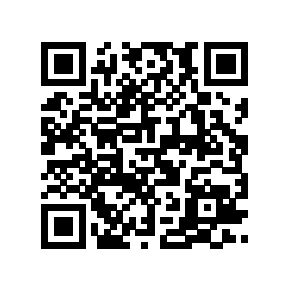
\includegraphics{qr}
  \centering
\end{figure}

\newpage
%后记
%% \chapter*{参考文献}
\bibliographystyle{gbt7714-numerical}  % 参考文献用
\bibliography{cankaowenxian}

\end{document}